\chapter{Programming Constructs}

Computer programs are made up of a strict sequence of instructions. Such sequences are called an algorithm. We, humans, run various algorithms every day as part of our daily lives. Getting ready and going to school is an algorithm. We wake up, get dressed, do our morning outfit, have breakfast, leave the house, and move to school. A very vivid example of an algorithm is cooking recipes. There are starting products in a recipe, then precise instructions on how to process and mix the products, with a clear idea of the end result. In computer programs, a basic set of instructions make up the means of expression of the corresponding programming language. The charm of block languages is that this basic set of instructions is represented visually in the form of colored blocks. The arrangement of the colored blocks in a strictly defined sequence leads to the creation of small computer programs.

In the case of Scratch, the program has well-defined start and end points. With App Inventor, the approach is slightly different. There, the sequence of instructions that make up the written program is entered in small fragments called events. Events are triggered by various user or operating system actions. In Scratch, we talk about sequential programming; in App Inventor, we talk about event programming. The basic programming constructs in the two programming environments are identical, but there are also some significant differences. To write efficient and reliable programs, knowing the means of expression of our programming environments is essential. 

\section{Programming Constructs in Scratch}

The basic building blocks in Scratch are organized into colored groups (Fig. \ref{fig020001}). This organization helps to navigate faster and use the different blocks more efficiently.

\begin{figure}[H]
   \centering
   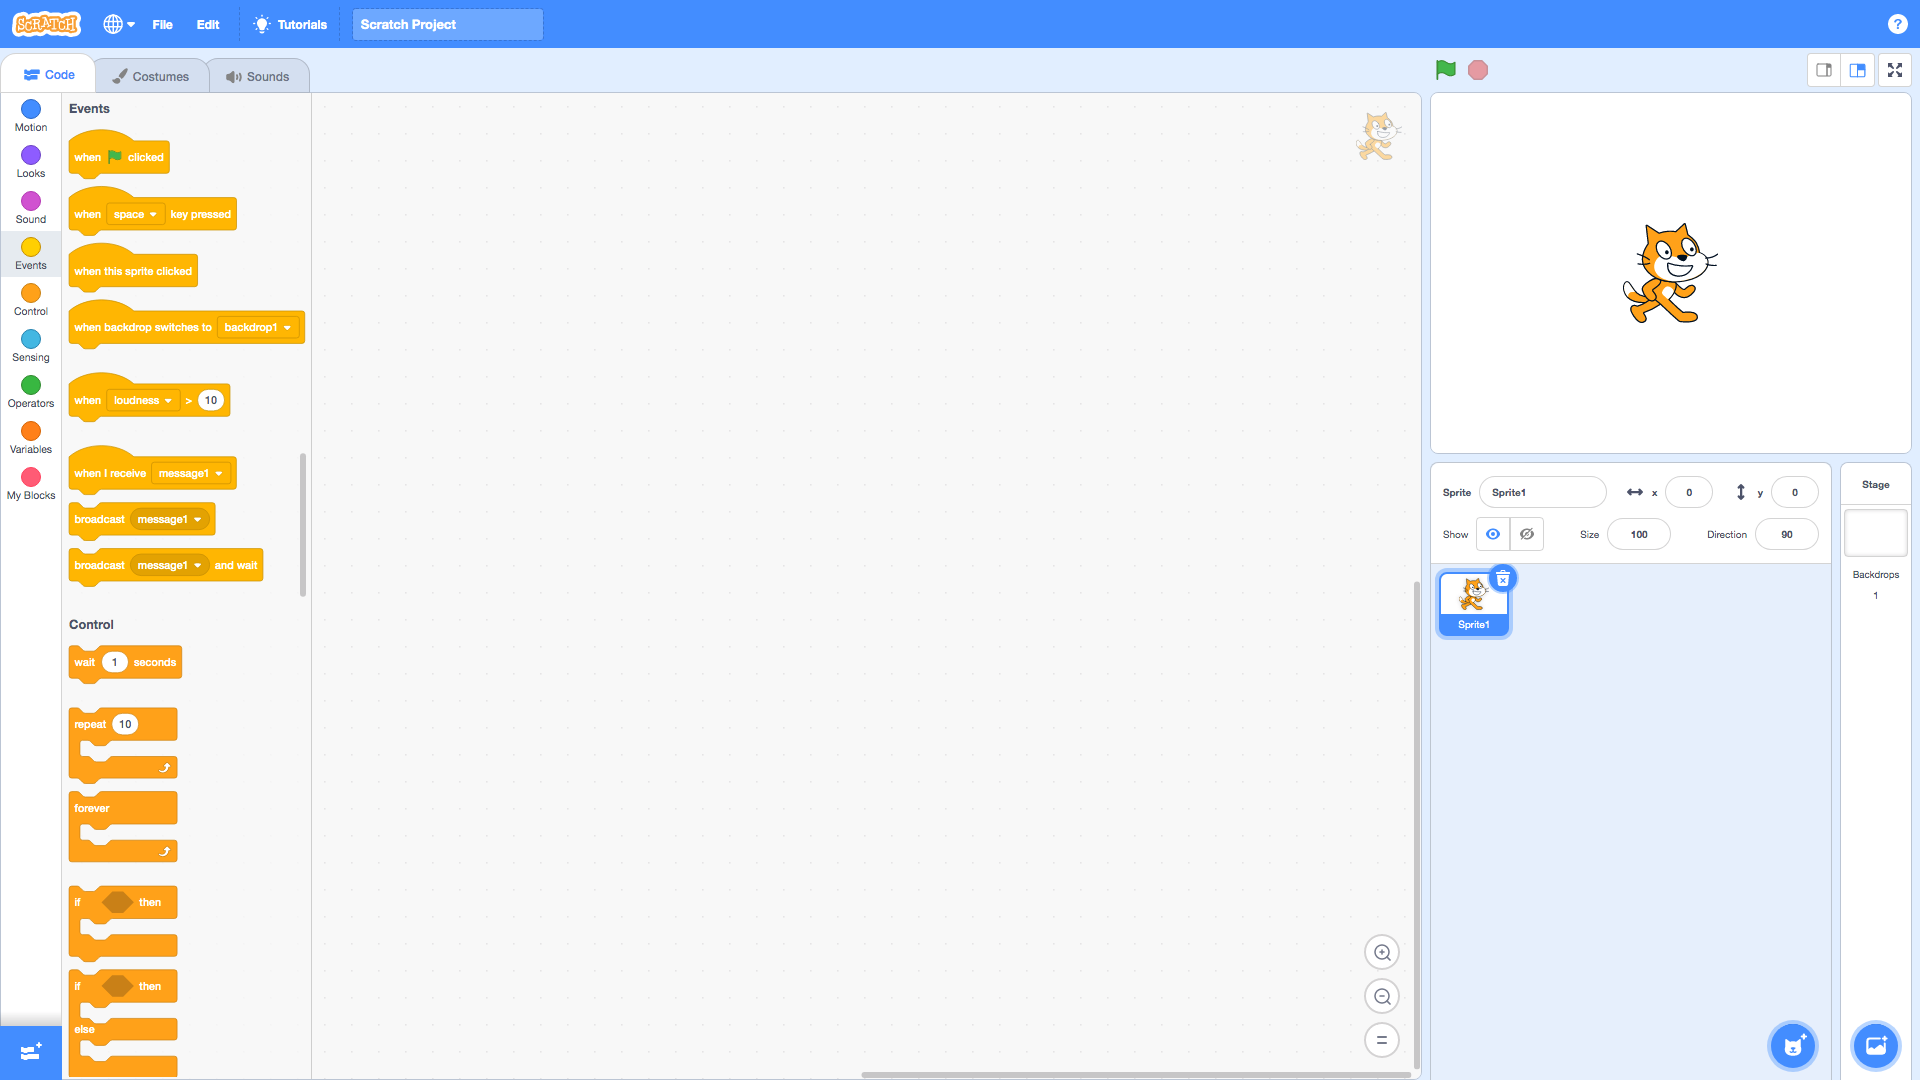
\includegraphics[width=1.0\linewidth,height=0.5\linewidth]{fig020001.png}
   \caption{Grouping instructions}
\label{fig020001}
\end{figure}

The most significant block in the program is the block that initiates the execution of the instructions arranged below it. This block has a green flag (Fig. \ref{fig020002}) and defines what will happen after the program is started.

\begin{figure}[H]
   \centering
   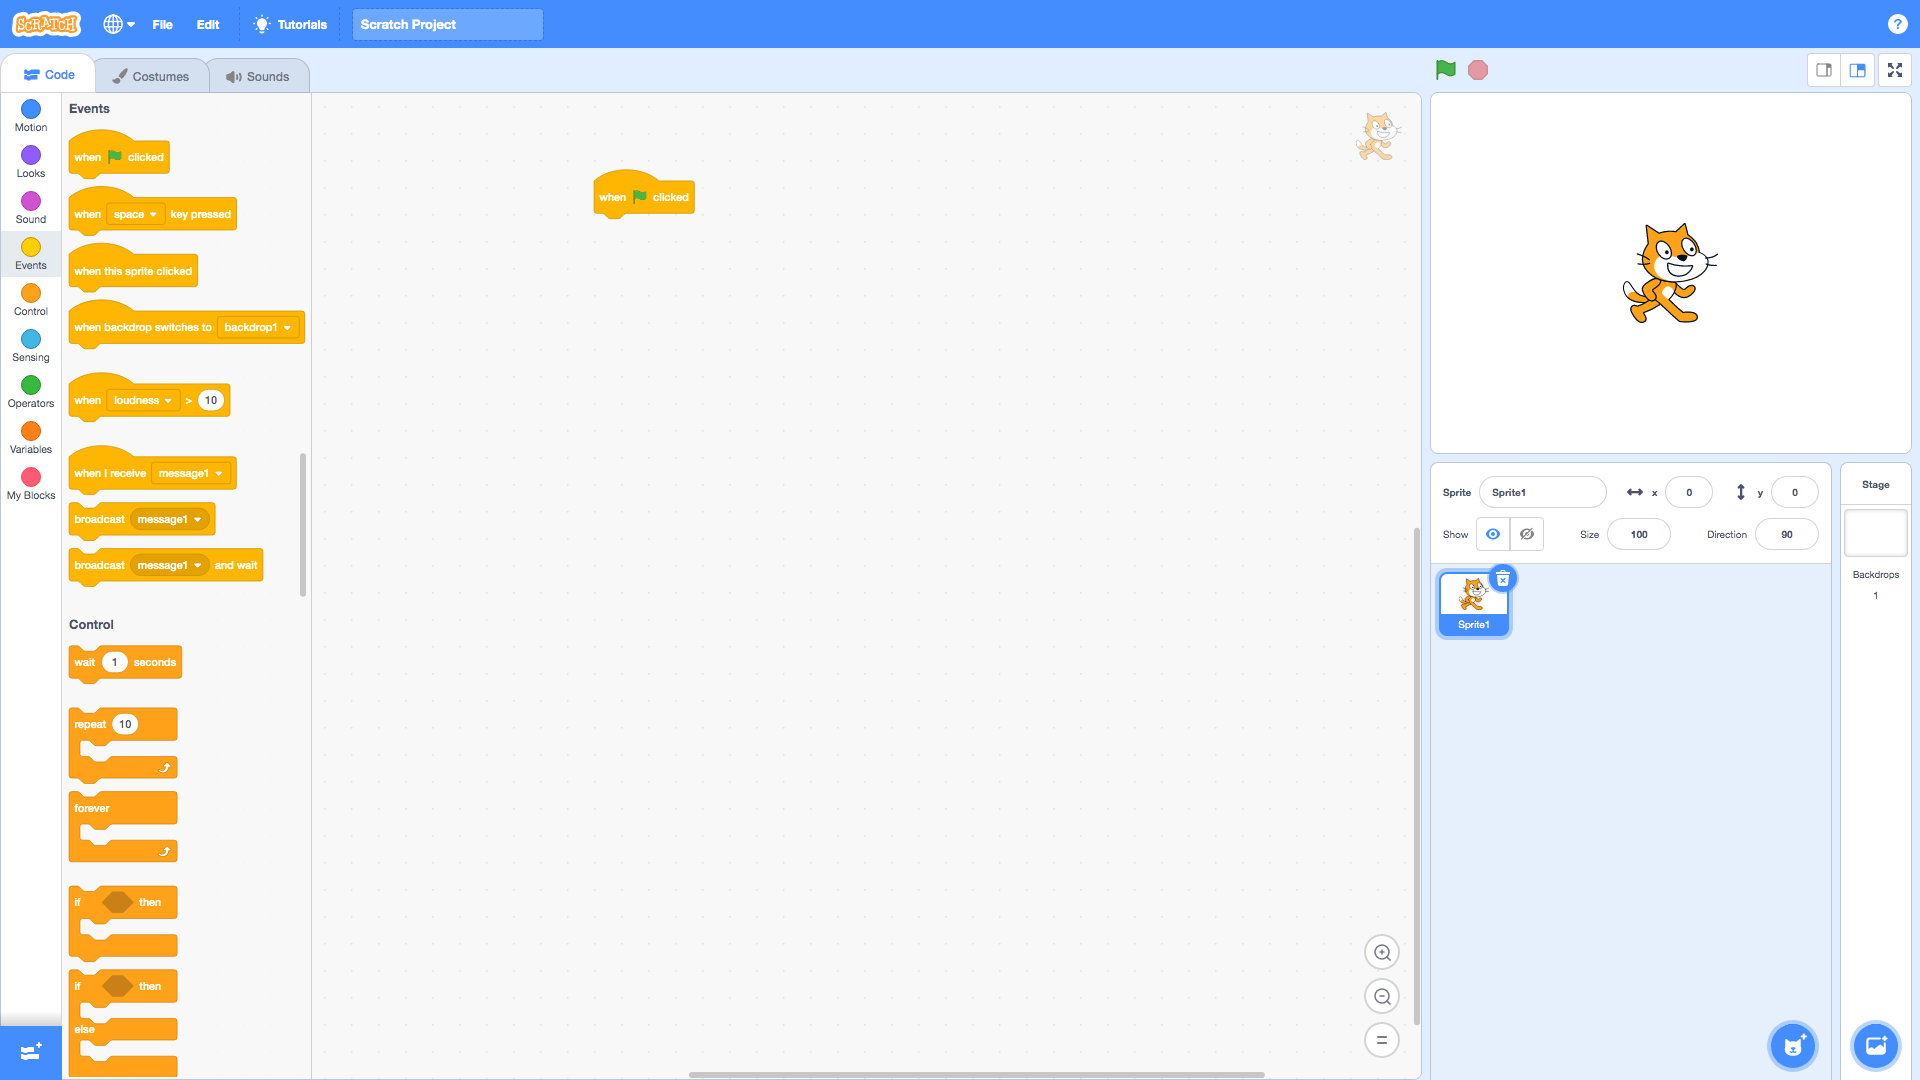
\includegraphics[width=1.0\linewidth,height=0.5\linewidth]{fig020002.png}
   \caption{Starting point of the program}
\label{fig020002}
\end{figure}

The program launch block is in the light orange group, designed to react to user events. The exact moment the user wants the program to start its execution is undefined in time, so Scratch must catch an event triggered by the user himself.

The second most significant block ends the program (Fig. \ref{fig020003}). It is located in the dark orange group and has the task of stopping all processes taking place during the execution of the program itself.

\begin{figure}[H]
   \centering
   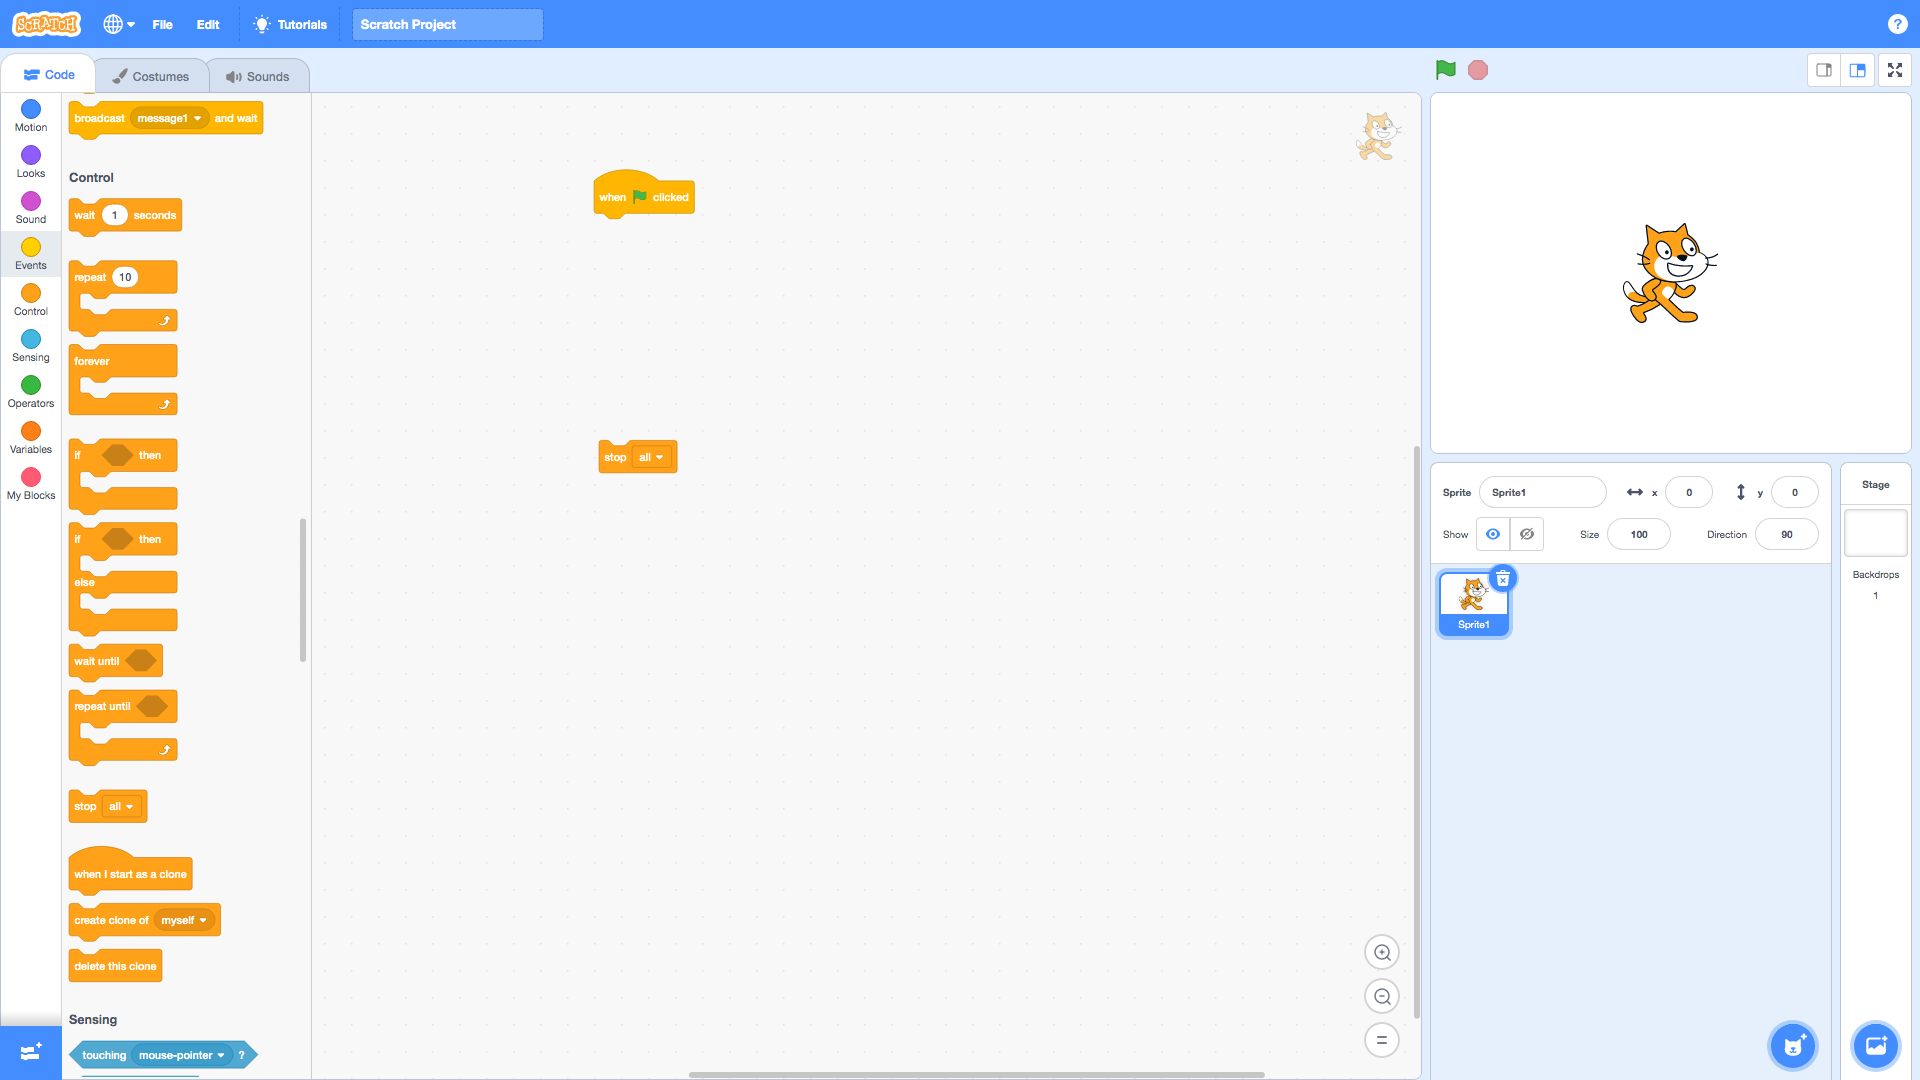
\includegraphics[width=1.0\linewidth,height=0.5\linewidth]{fig020003.png}
   \caption{Program endpoint}
\label{fig020003}
\end{figure}

The dark orange group contains performance control blocks. These blocks allow the program to take different paths and a group of actions to be repeated many times.

In Scratch, instruction blocks basically control pictures called sprites. Unlike an ordinary computer image, a sprite is a graphic object containing multiple frames showing the character's image in different configurations. Every new Scratch program starts with a single sprite of the orange cat, located at coordinates (x=0,y=0). The workspace is a two-dimensional coordinate system centered at (0,0).

\begin{figure}[H]
   \centering
   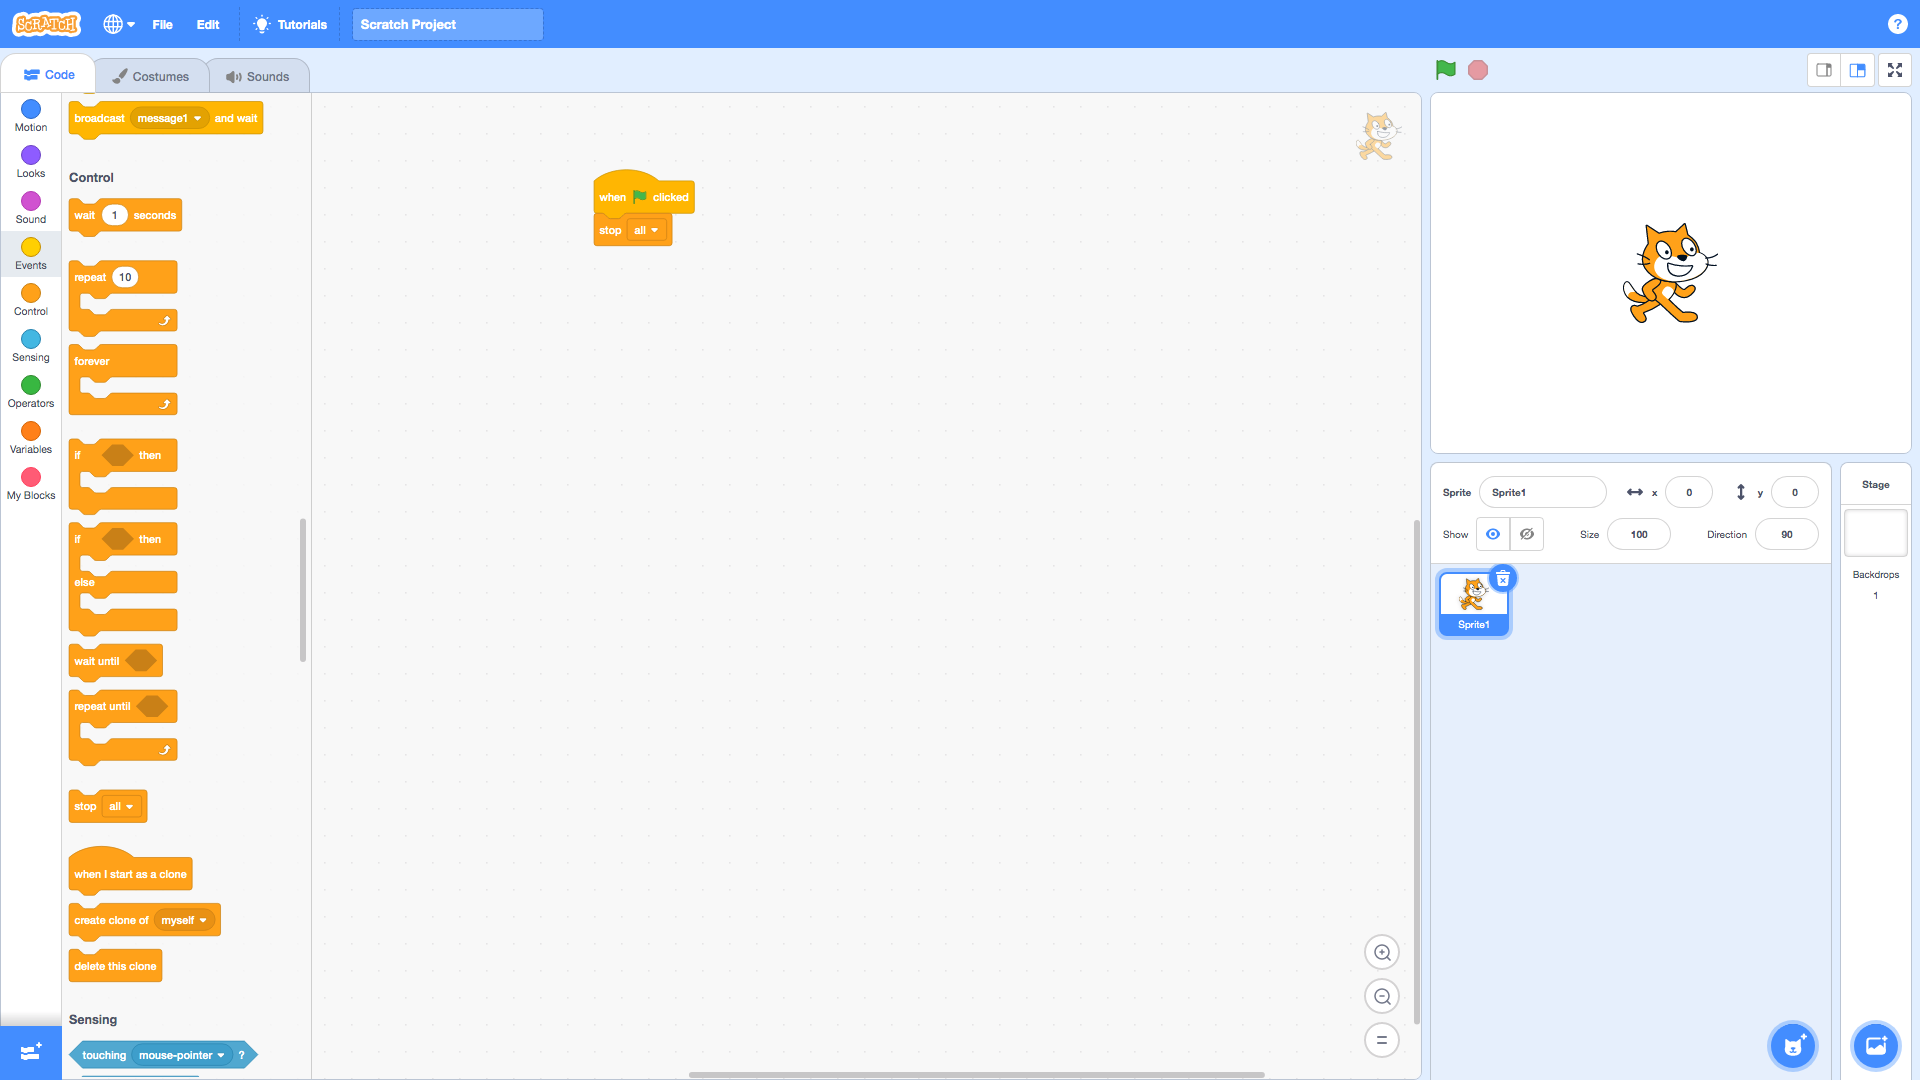
\includegraphics[width=1.0\linewidth,height=0.5\linewidth]{fig020004.png}
   \caption{Finish immediately after starting}
\label{fig020004}
\end{figure}

The program does nothing if the start and end blocks are joined (Fig. \ref{fig020004}). Practically, this program ends as soon as it starts. A program that does nothing is entirely pointless. To start something happening, use the blocks in the blue group. The first block instructs the kitten to move 10 steps, and the number of steps can be changed by writing another number inside the block (Fig. \ref{fig020005}).

\begin{figure}[H]
   \centering
   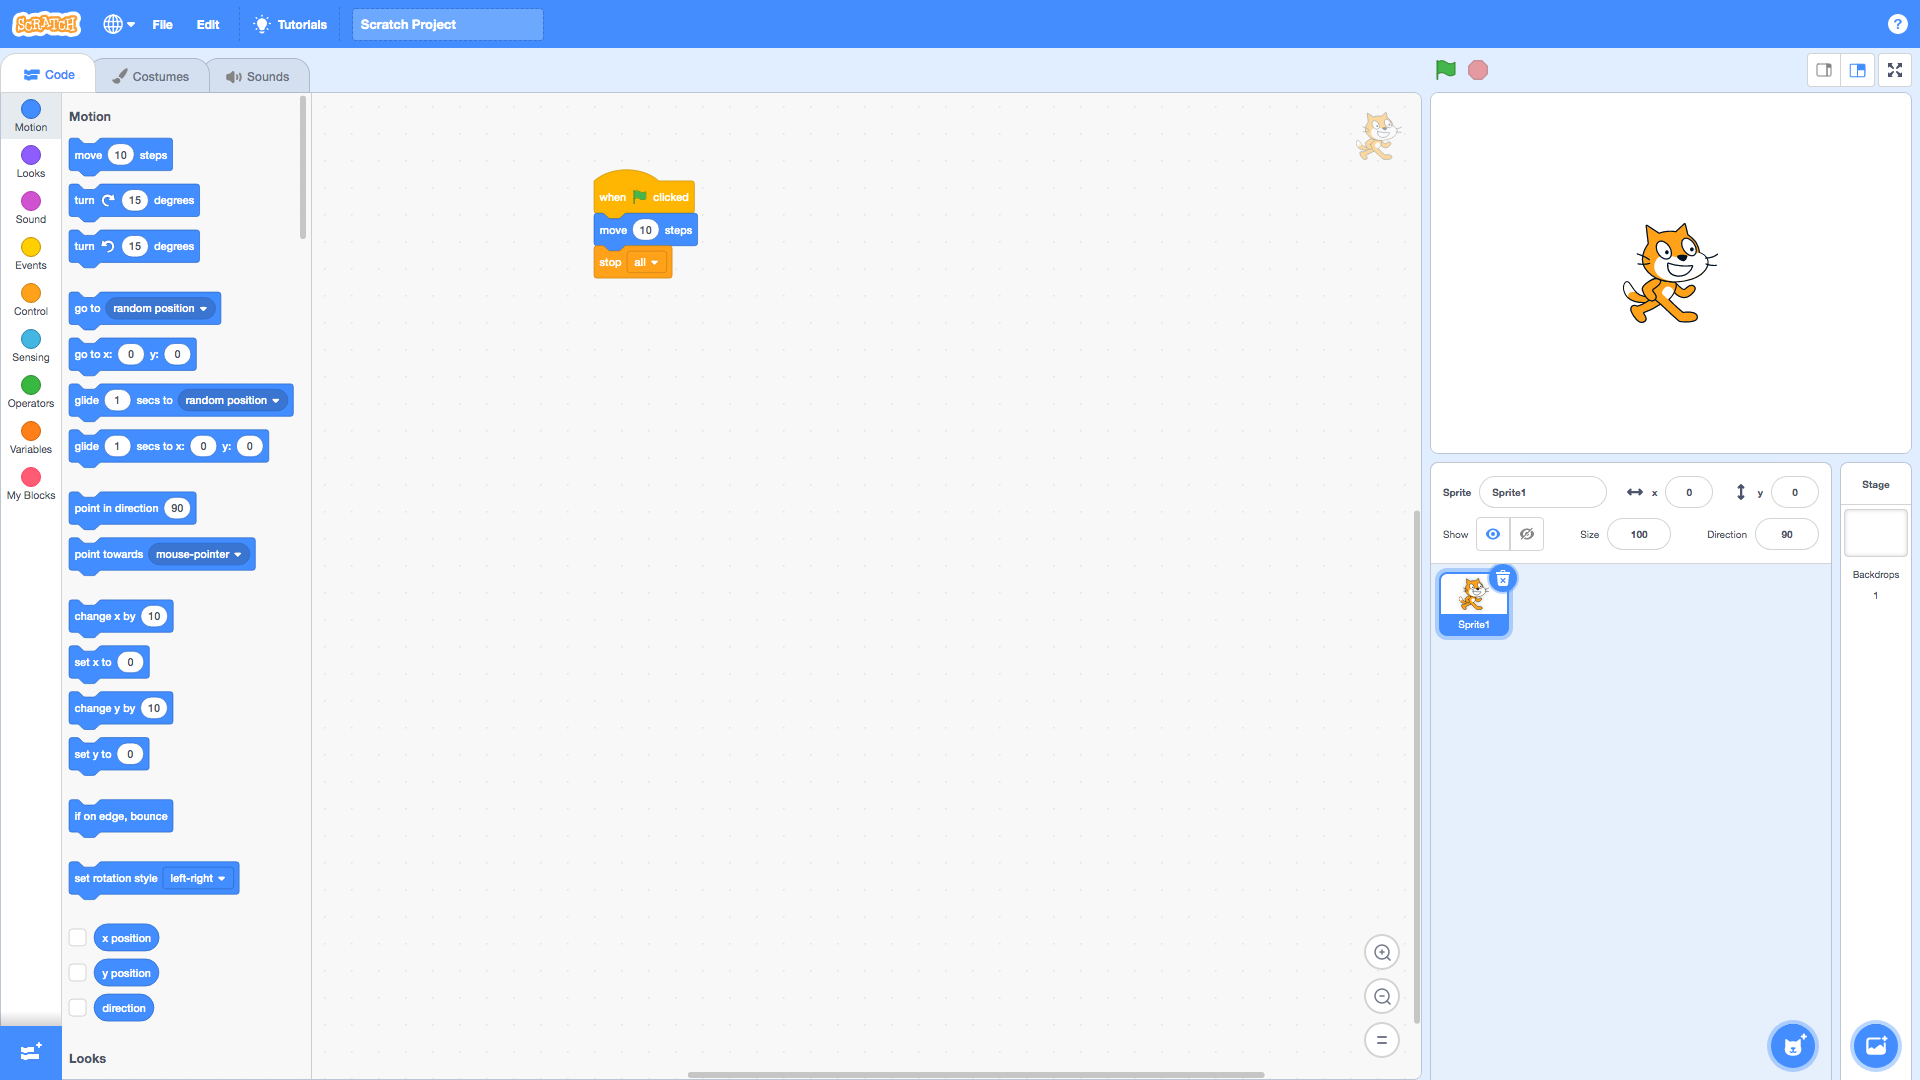
\includegraphics[width=1.0\linewidth,height=0.5\linewidth]{fig020005.png}
   \caption{Moving character}
\label{fig020005}
\end{figure}

The next block in the group instructs the character to rotate a specified number of degrees, clockwise, relative to its own center (Fig. \ref{fig020006}).

\begin{figure}[H]
   \centering
   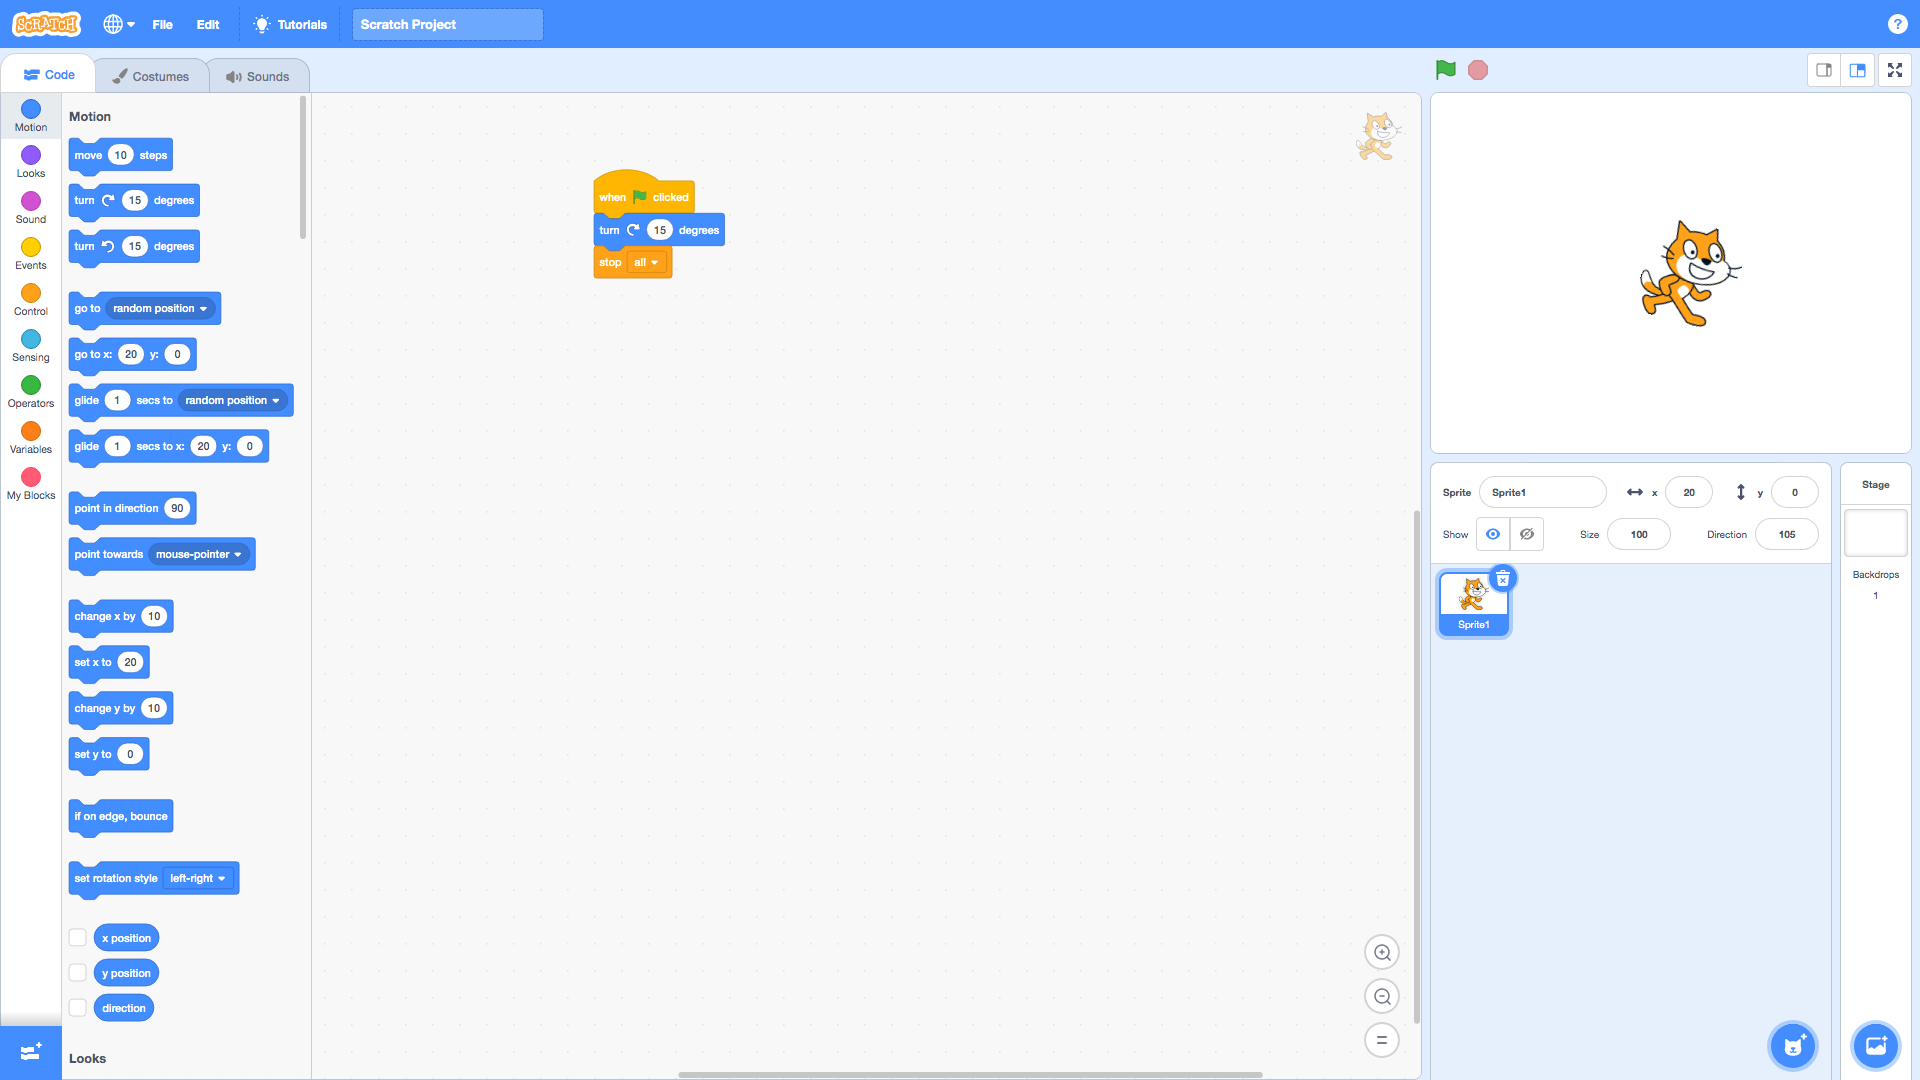
\includegraphics[width=1.0\linewidth,height=0.5\linewidth]{fig020006.png}
   \caption{Clockwise Rotation}
\label{fig020006}
\end{figure}

Similarly, with the next block in the group, the rotation can be performed counterclockwise (Fig. \ref{fig020007}).

\begin{figure}[H]
   \centering
   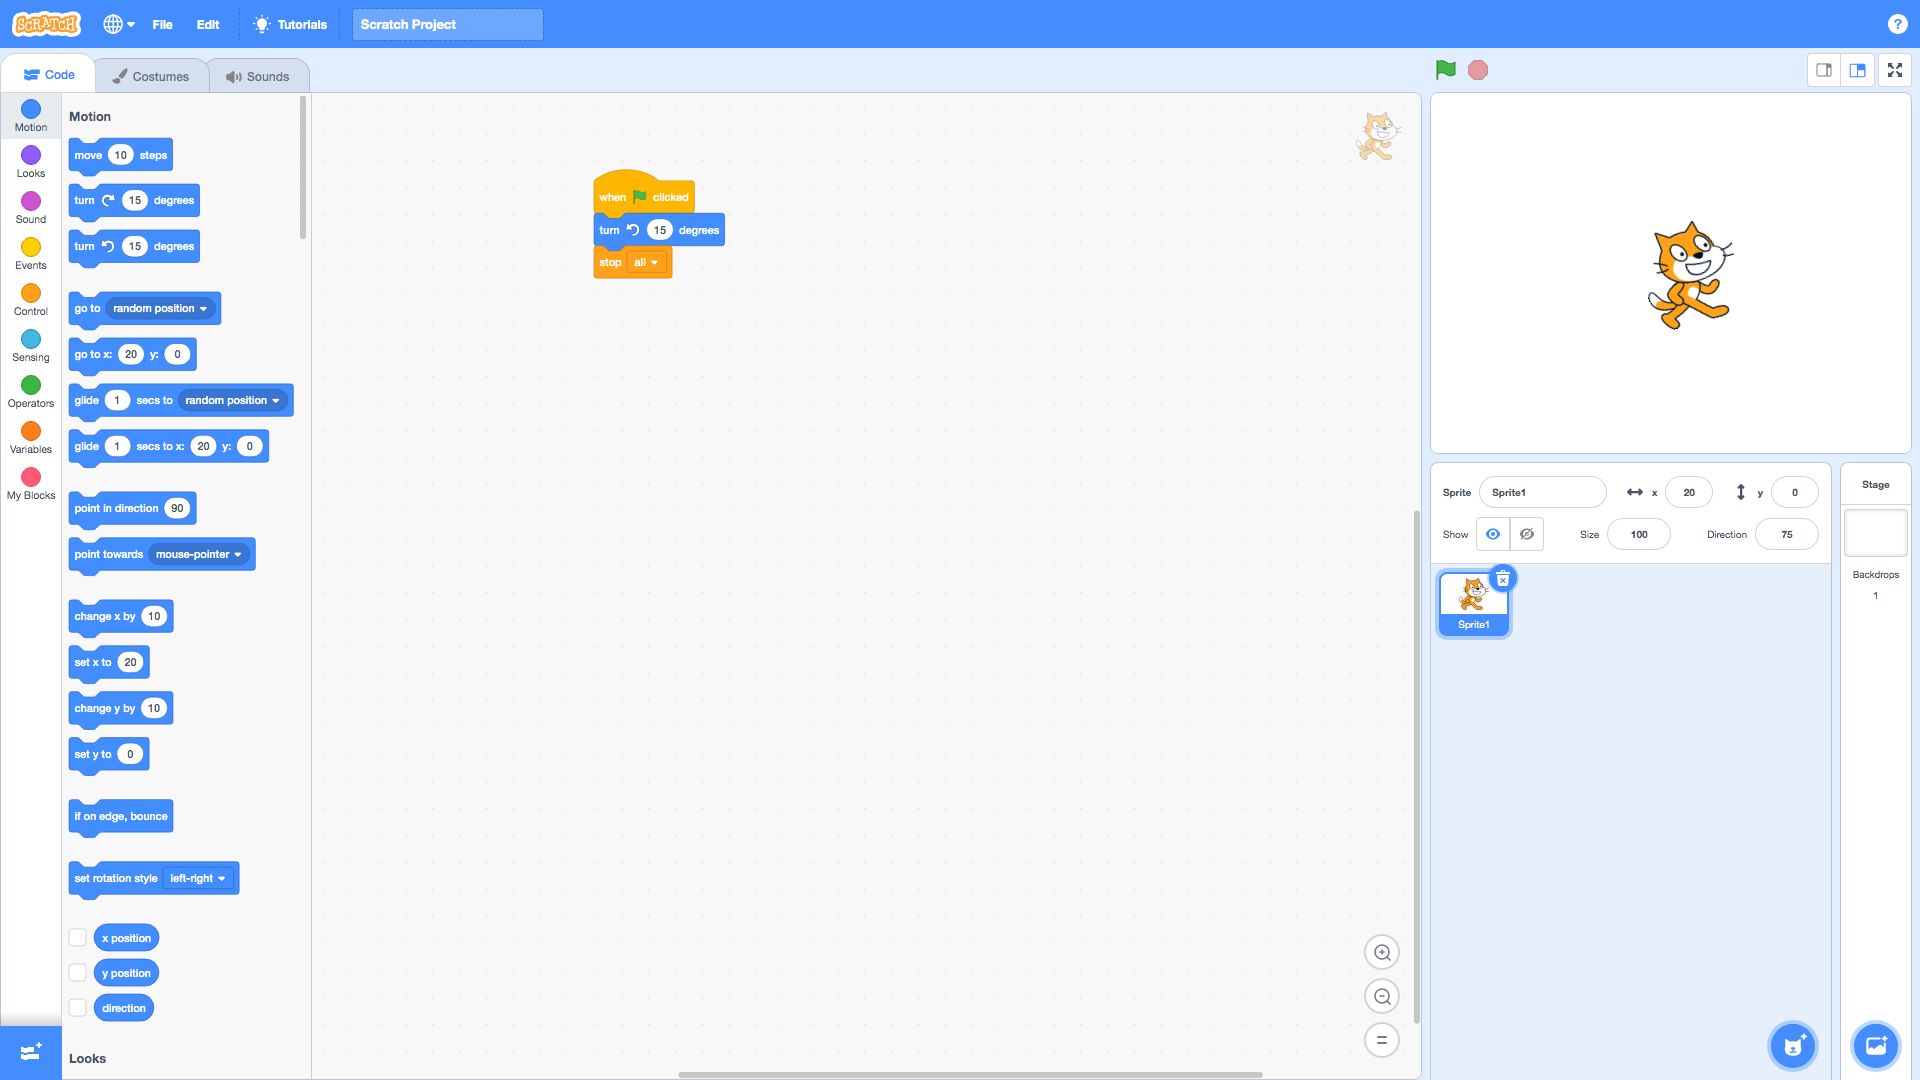
\includegraphics[width=1.0\linewidth,height=0.5\linewidth]{fig020007.png}
   \caption{Counterclockwise Rotation}
\label{fig020007}
\end{figure}

The next block in the group allows the character to move to random coordinates or coordinates specified with the mouse (Fig. \ref{fig020008}).

\begin{figure}[H]
   \centering
   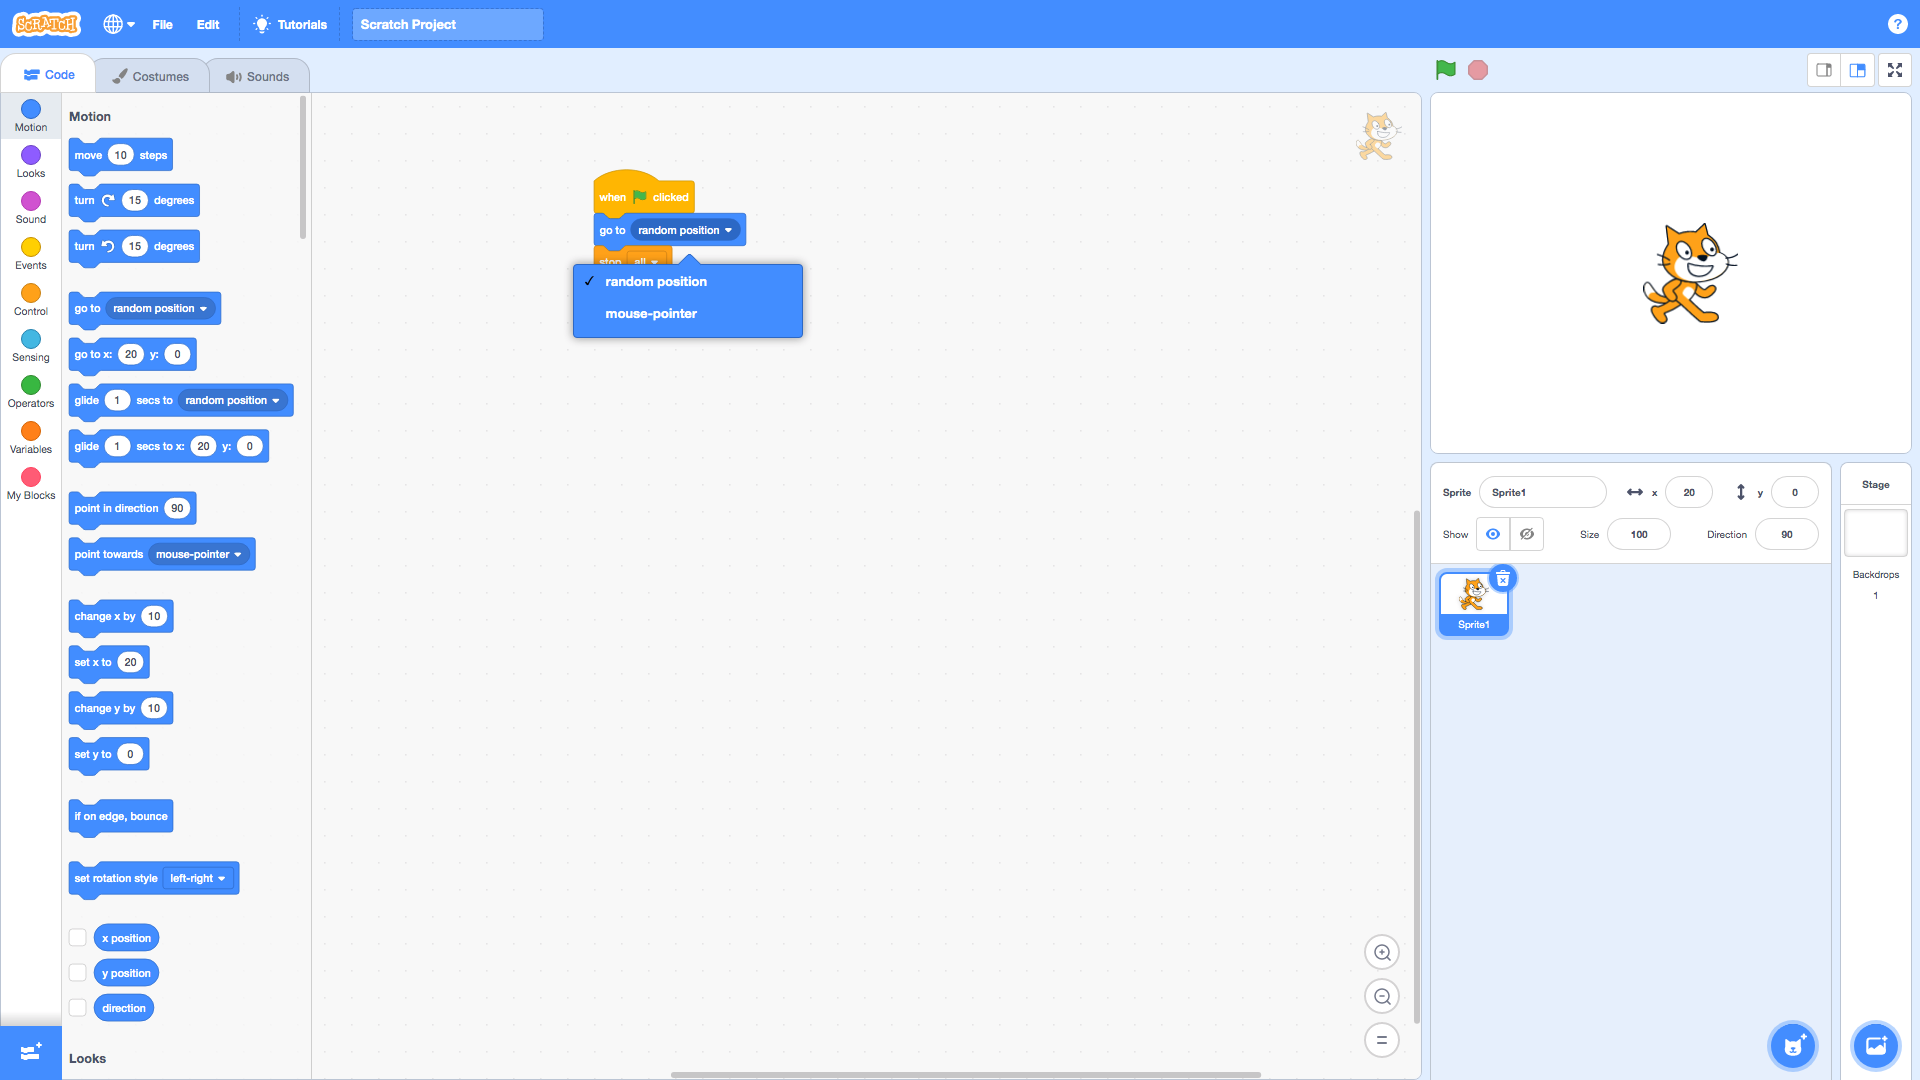
\includegraphics[width=1.0\linewidth,height=0.5\linewidth]{fig020008.png}
   \caption{Move to random position}
\label{fig020008}
\end{figure}

The character's movement can also be set by absolute coordinates with a block allowing entering numbers for the abscissa and ordinate axis (Fig. \ref{fig020009}).

\begin{figure}[H]
   \centering
   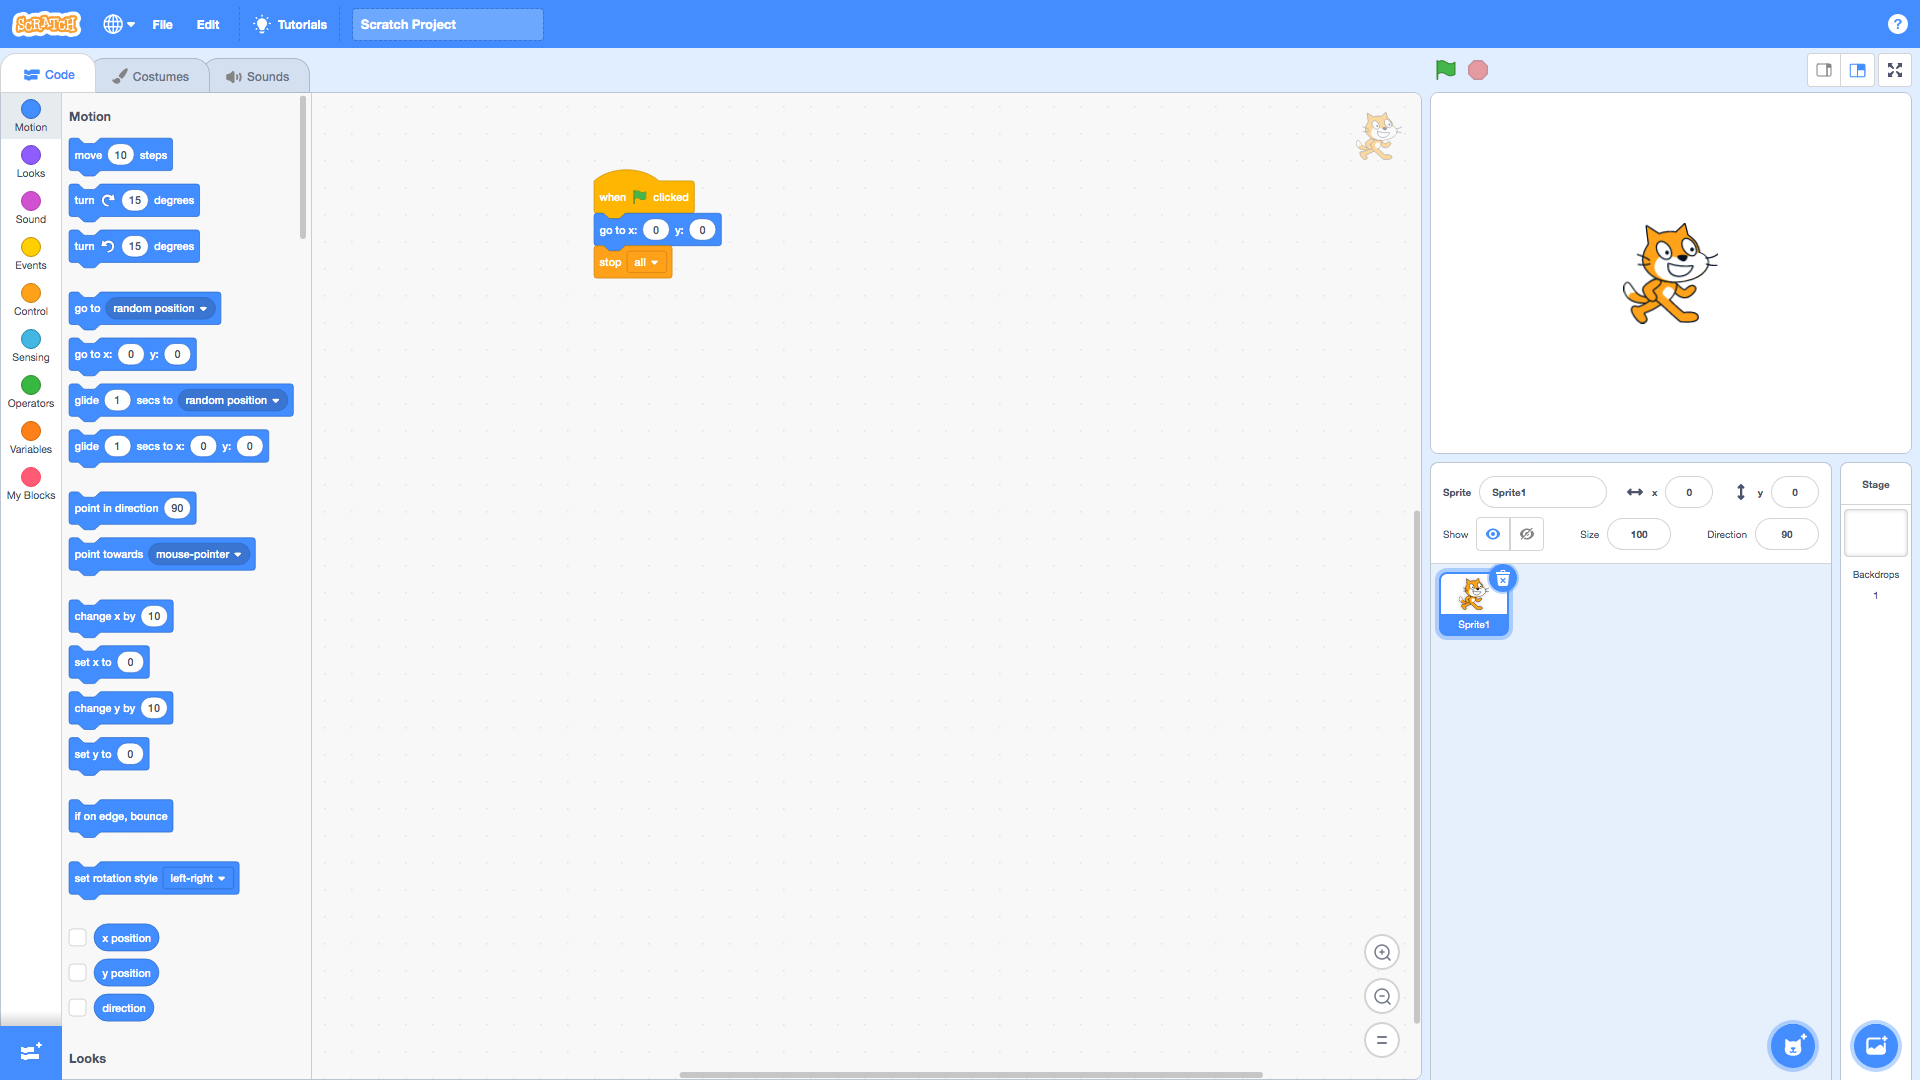
\includegraphics[width=1.0\linewidth,height=0.5\linewidth]{fig020009.png}
   \caption{Move by absolute coordinates}
\label{fig020009}
\end{figure}

Smooth movement at a predetermined time interval is possible at random coordinates or coordinates specified with the mouse, thanks to the next block in the group (Fig. \ref{fig020010}).

\begin{figure}[H]
   \centering
   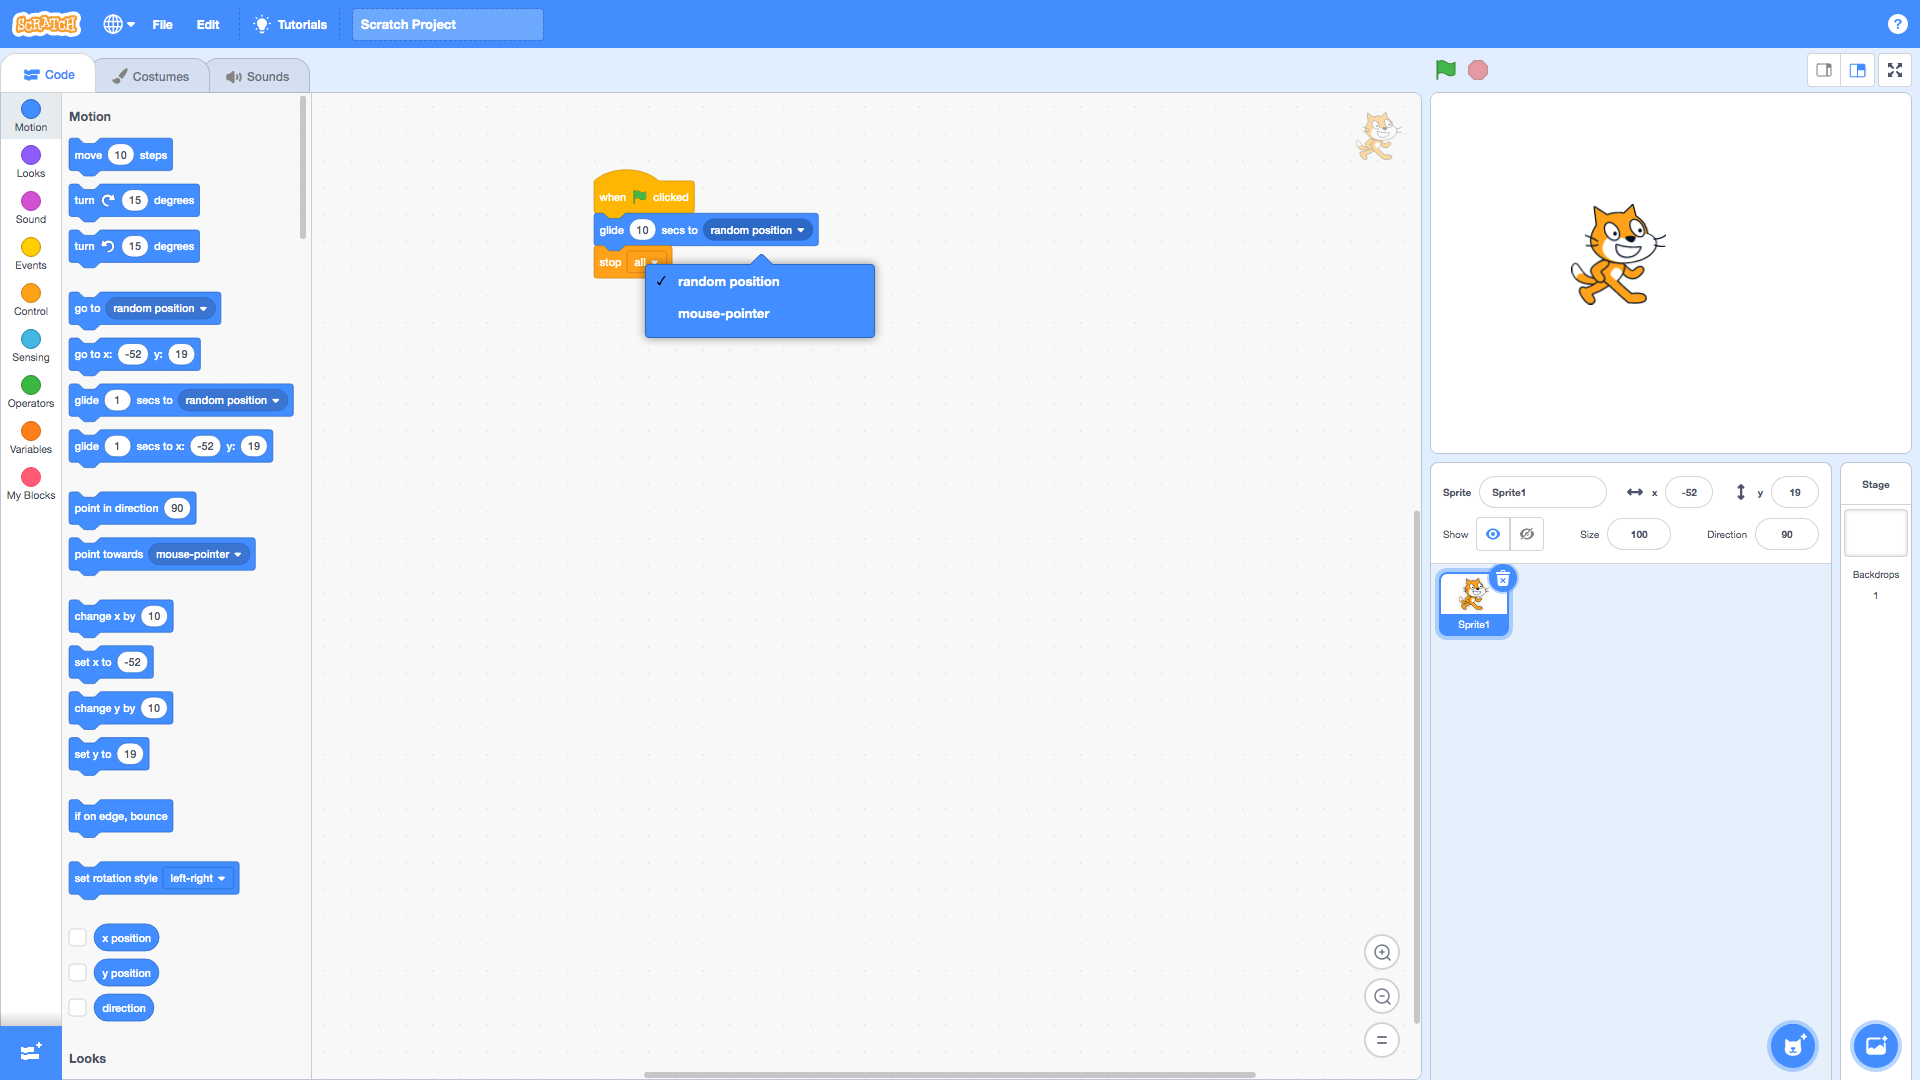
\includegraphics[width=1.0\linewidth,height=0.5\linewidth]{fig020010.png}
   \caption{Slide to random position}
\label{fig020010}
\end{figure}

Smooth sliding to predetermined coordinates for a predetermined time interval is possible with the block designed for this purpose (Fig. \ref{fig020011}).

\begin{figure}[H]
   \centering
   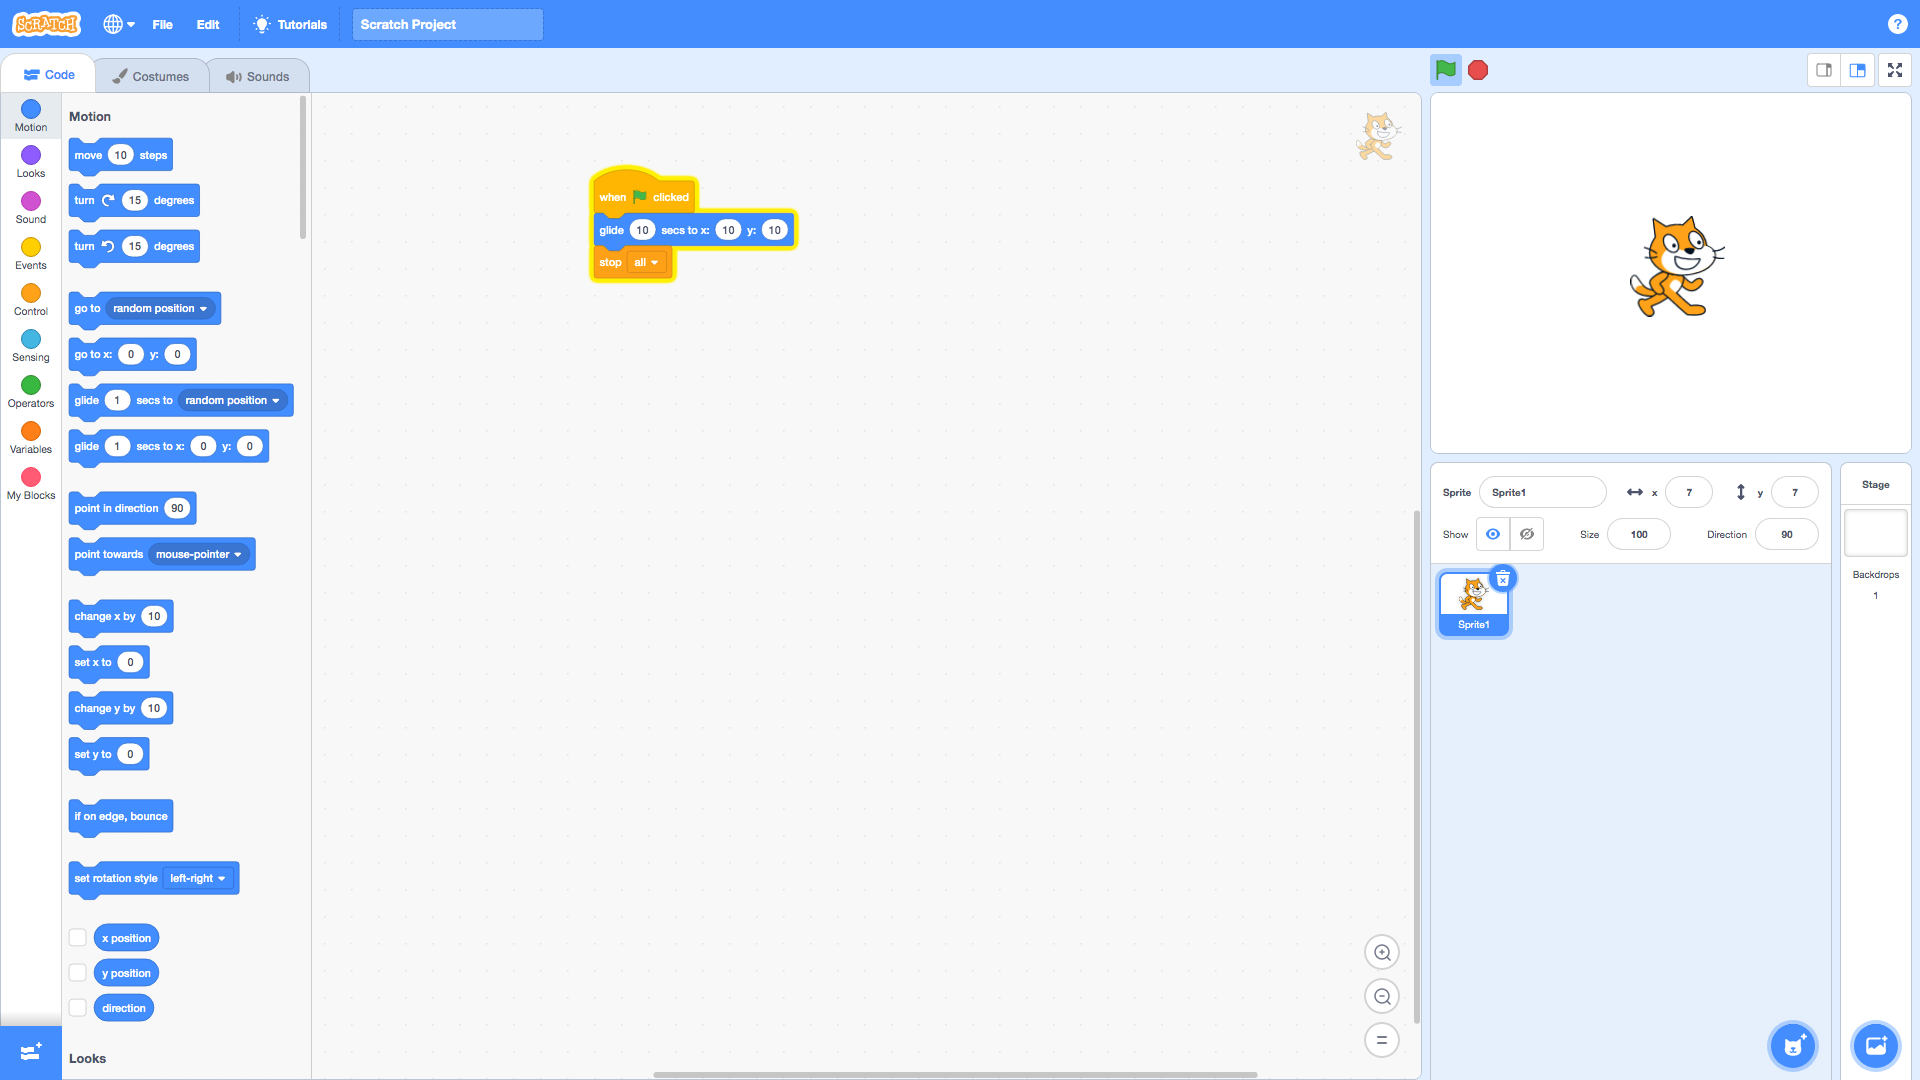
\includegraphics[width=1.0\linewidth,height=0.5\linewidth]{fig020011.png}
   \caption{Slide to set coordinates}
\label{fig020011}
\end{figure}

The animated character has an orientation property in the form of an angle. At 90 degrees, the orange cat is looking to the right. To change the character's orientation, a block with the possibility of entering a specific angle is used (Fig. \ref{fig020012}).

\begin{figure}[H]
   \centering
   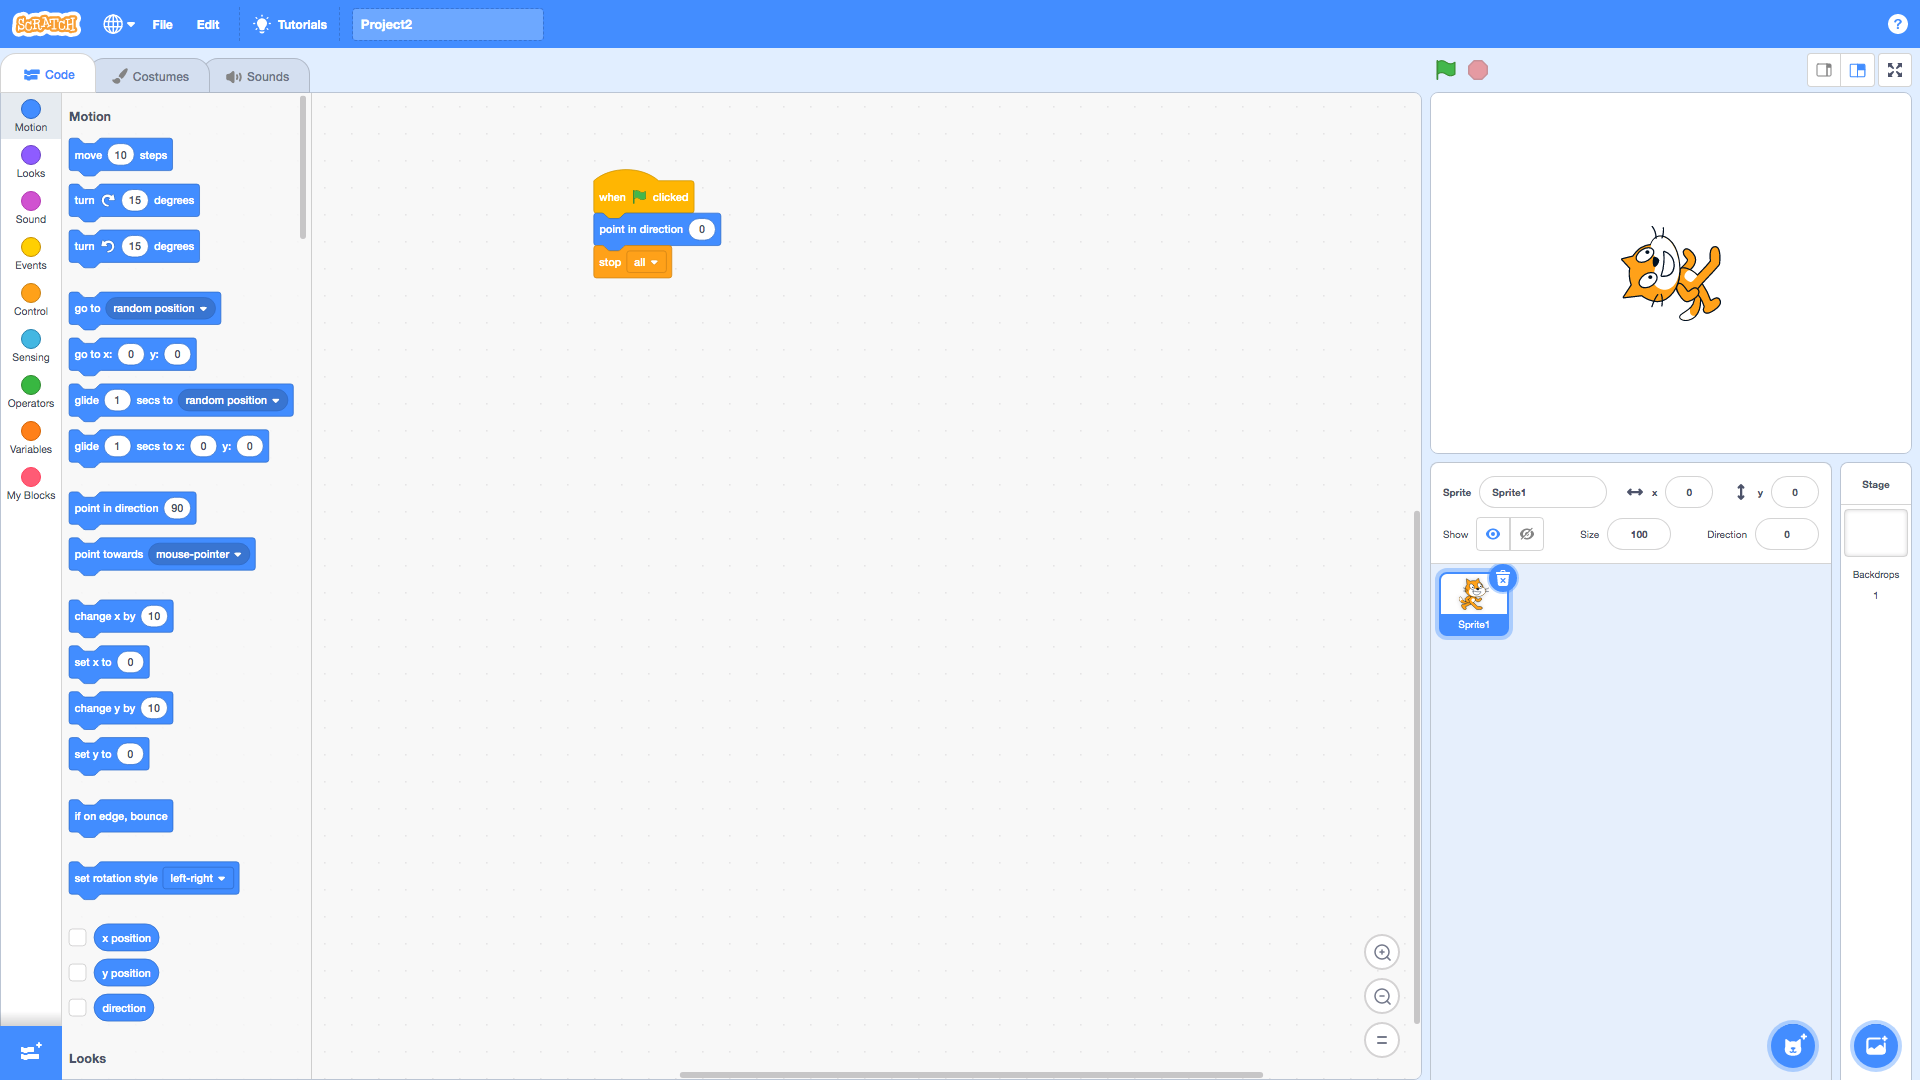
\includegraphics[width=1.0\linewidth,height=0.5\linewidth]{fig020012.png}
   \caption{Corner Orientation}
\label{fig020012}
\end{figure}

In more complex character control scenarios, sometimes the character needs to follow the mouse pointer. For this purpose, a specific block executes this instruction (Fig. \ref{fig020013}).

\begin{figure}[H]
   \centering
   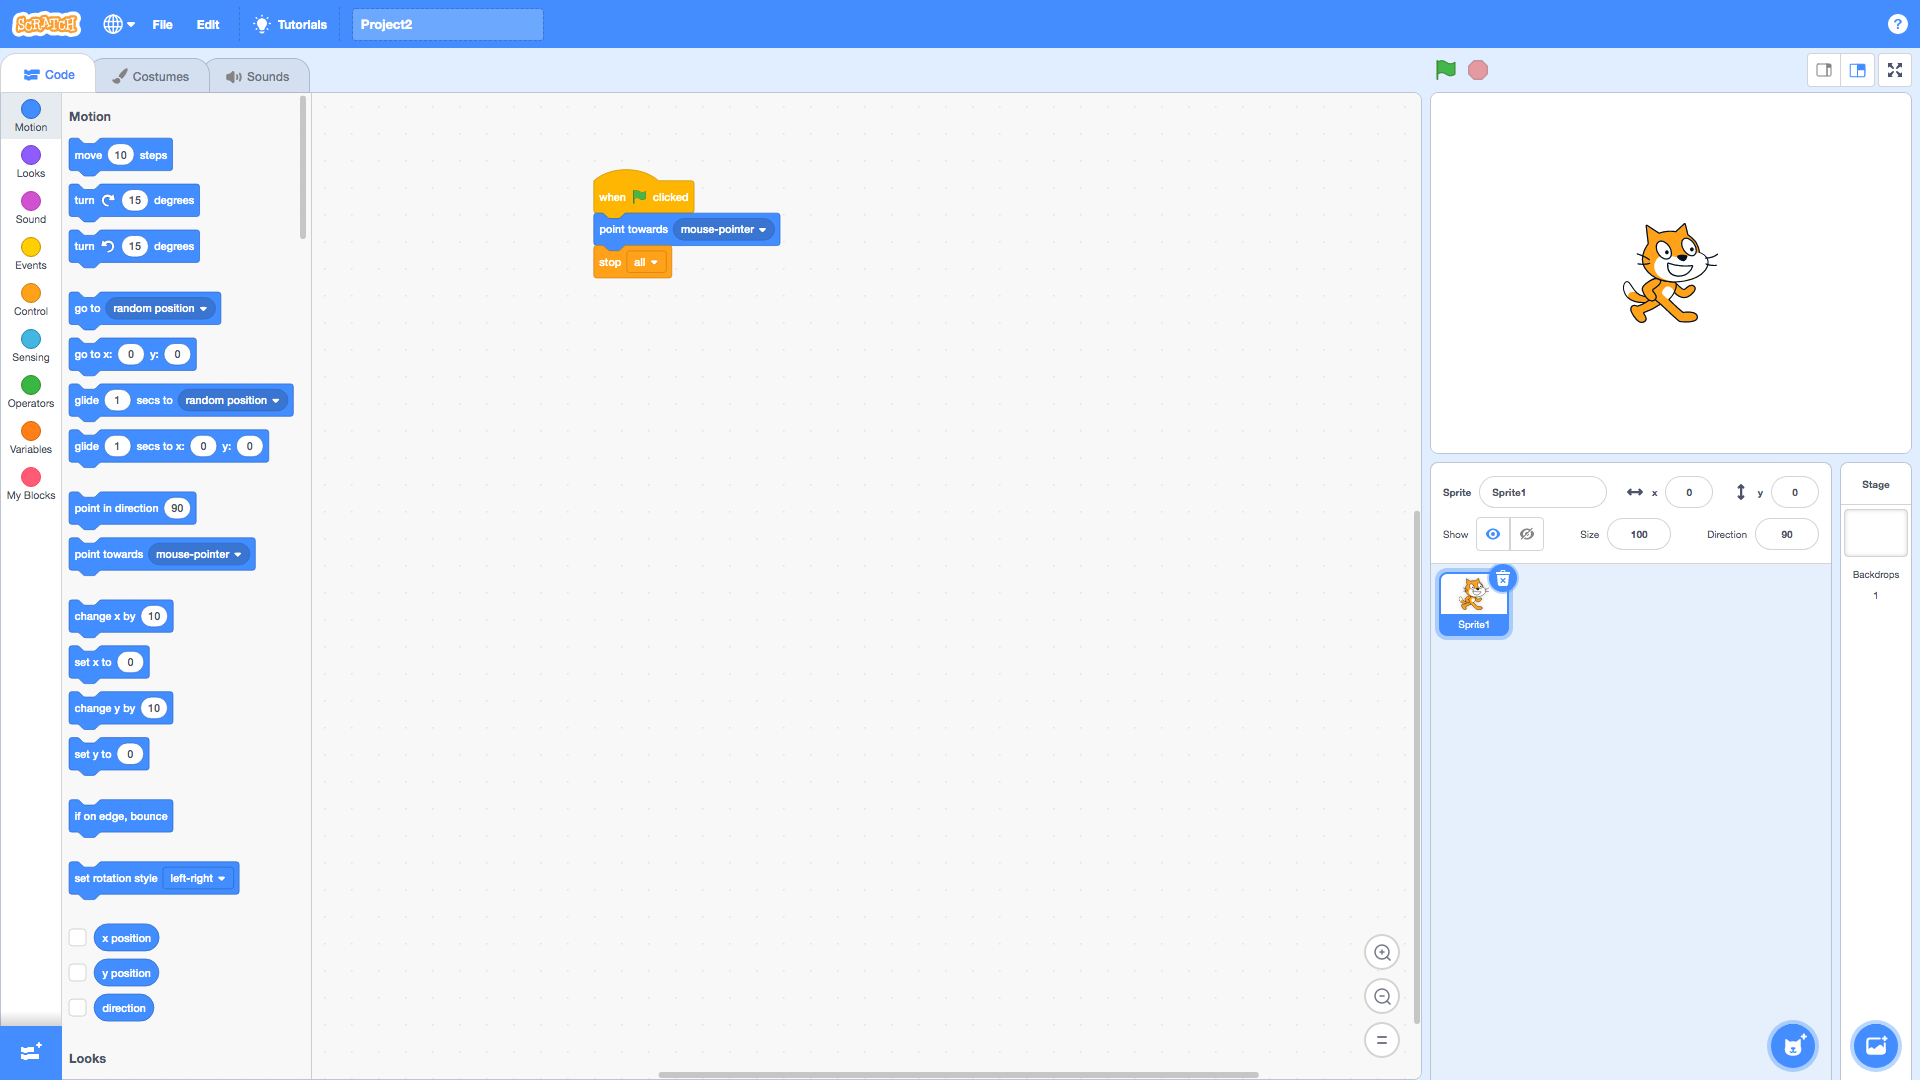
\includegraphics[width=1.0\linewidth,height=0.5\linewidth]{fig020013.png}
   \caption{Mouse Pointer Orientation}
\label{fig020013}
\end{figure}

Blocks can be placed one after the other, and for sequential change of the relative x and y coordinates (relative to the current position) of the character, there are specially defined blocks (Fig. \ref{fig020014}).

\begin{figure}[H]
   \centering
   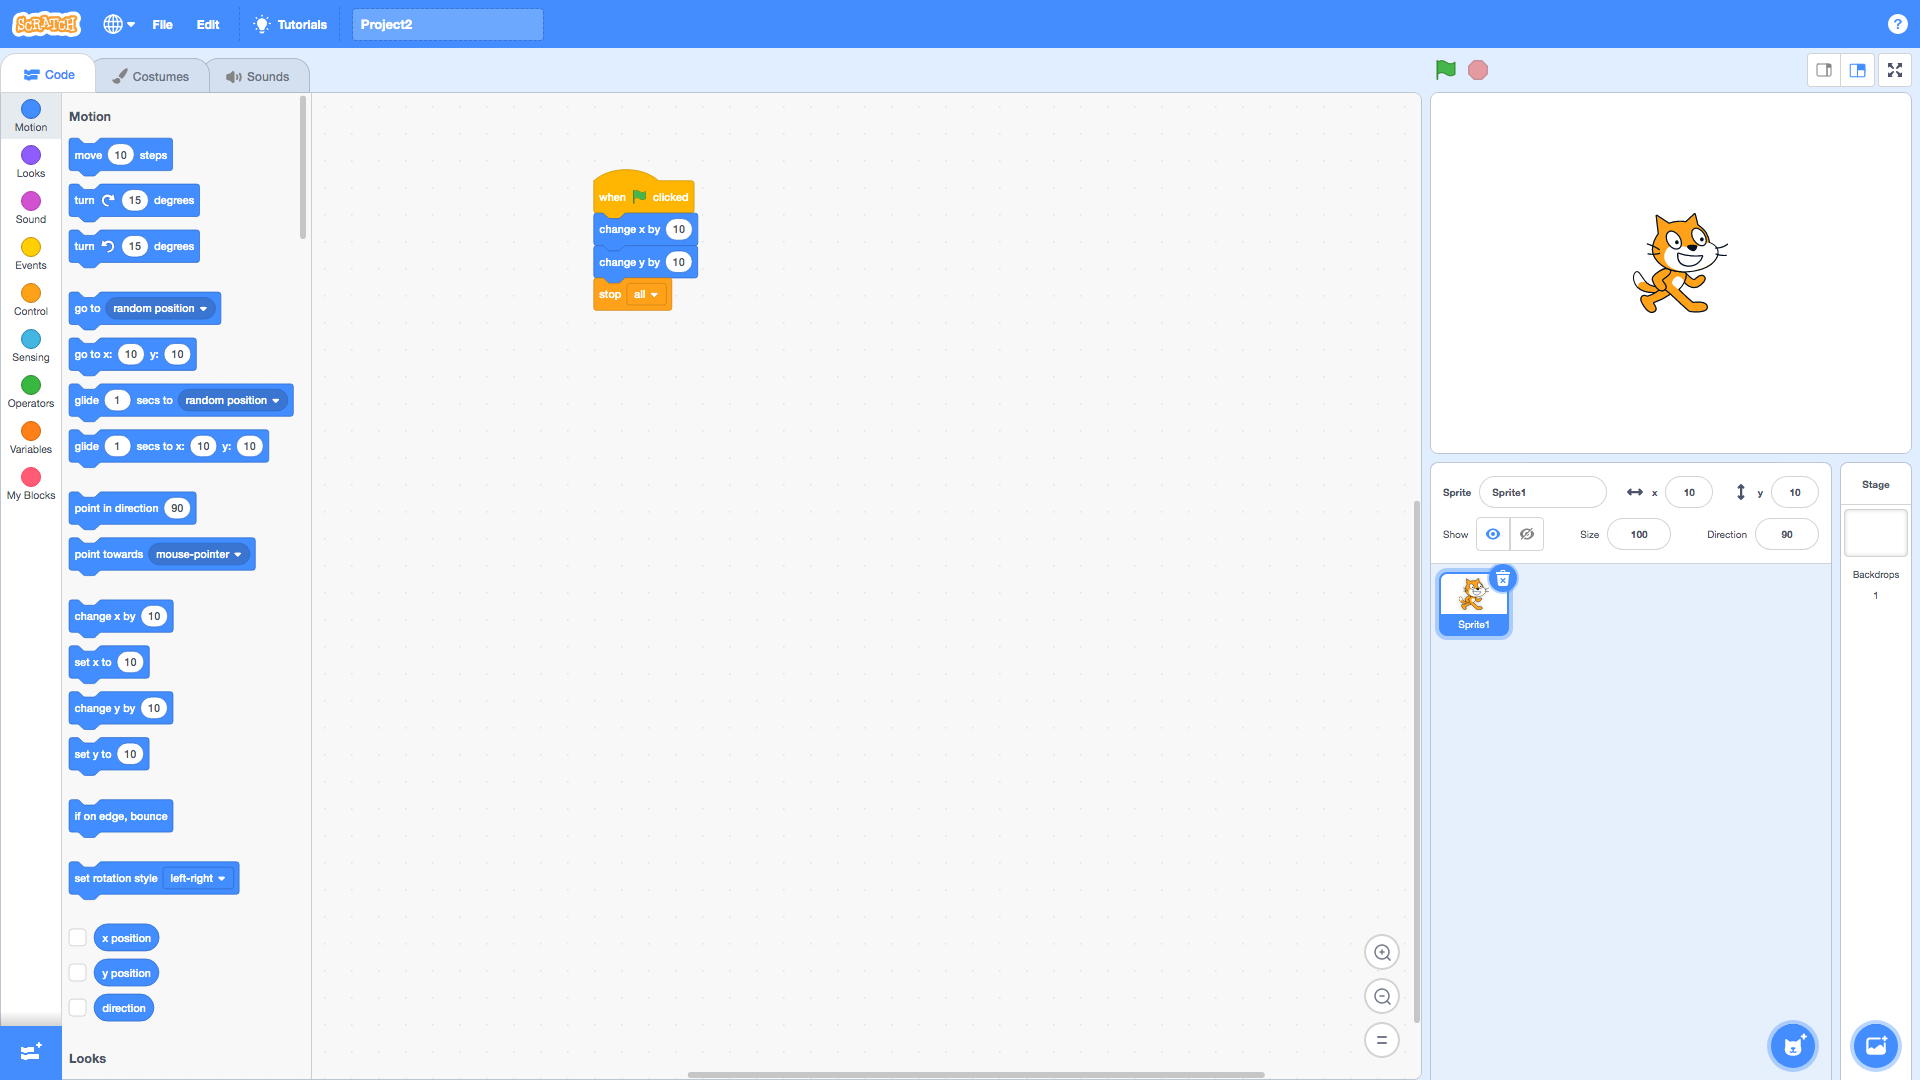
\includegraphics[width=1.0\linewidth,height=0.5\linewidth]{fig020014.png}
   \caption{Sequential change of relative coordinates}
\label{fig020014}
\end{figure}

In addition to a relative change of the coordinates, an absolute change of the coordinates is also possible, with the absolute change relative to the center of the coordinate system (Fig. \ref{fig020015}).

\begin{figure}[H]
   \centering
   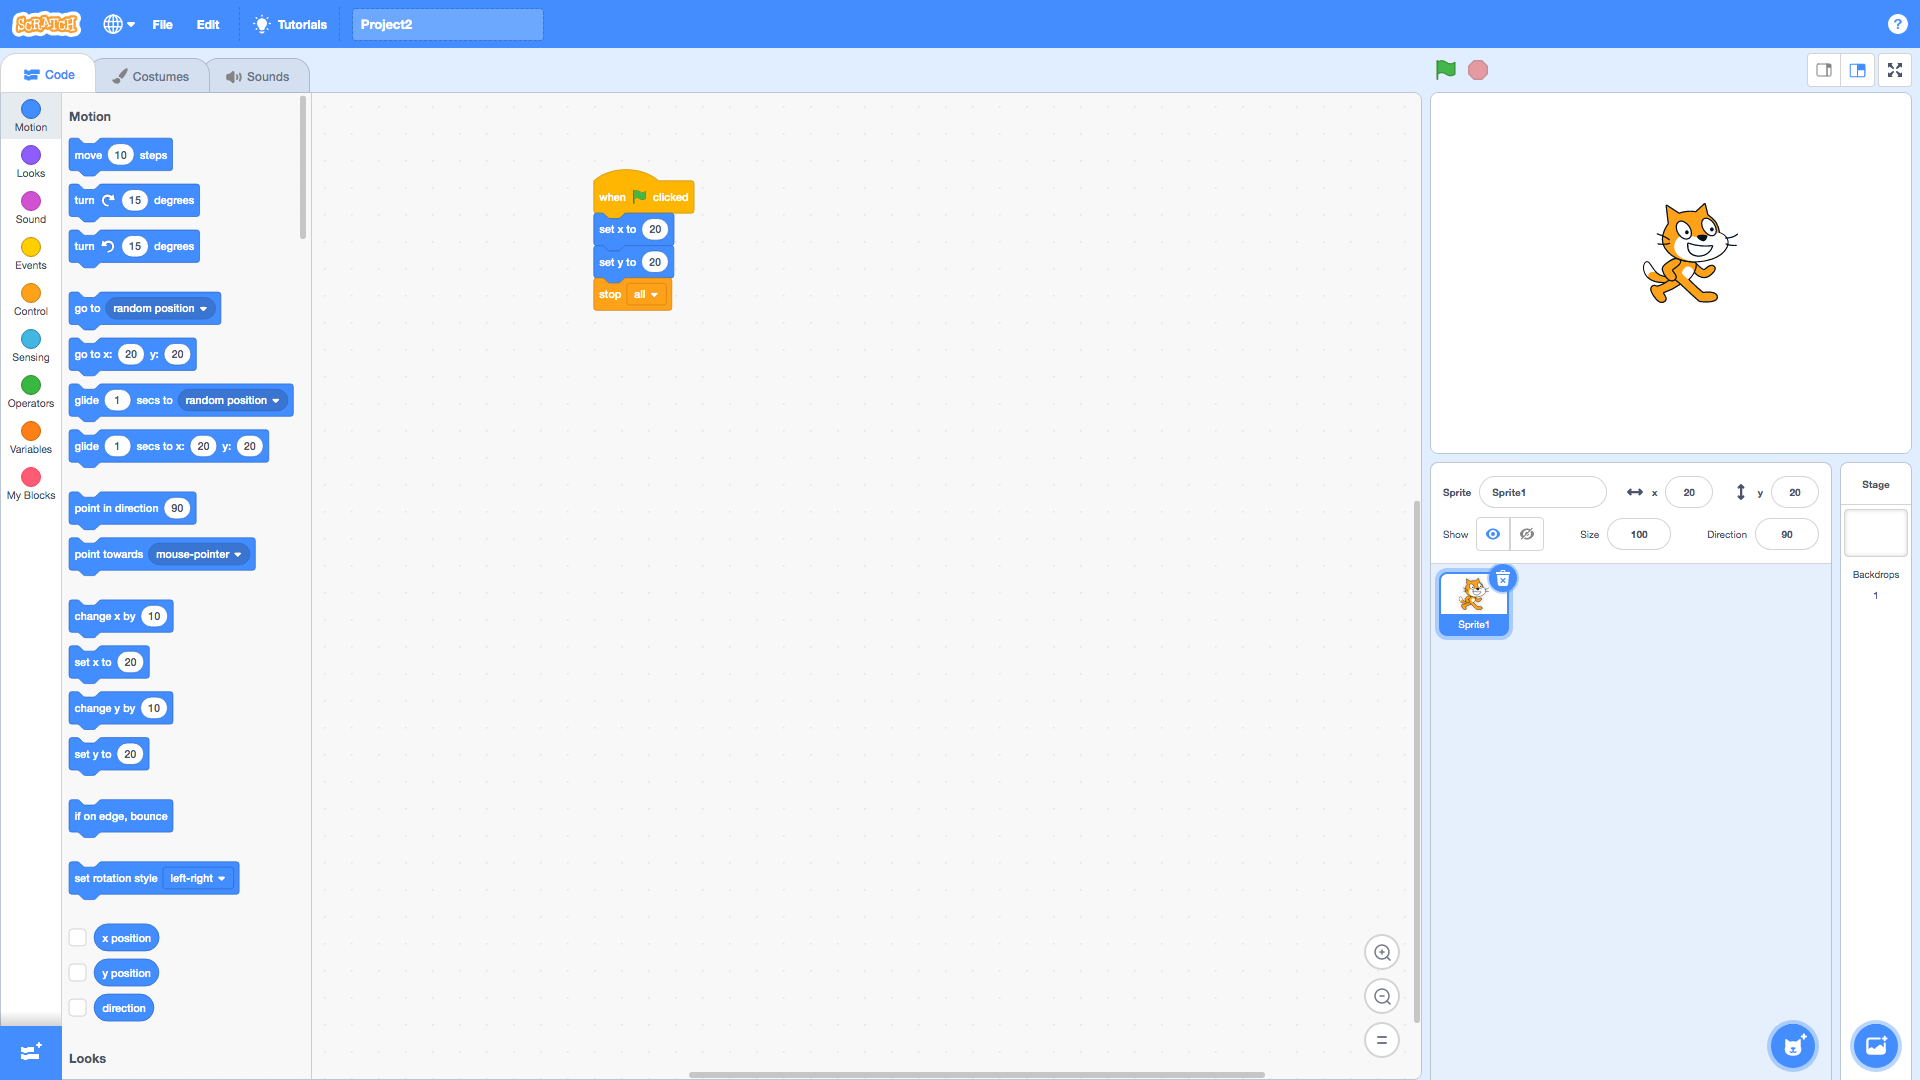
\includegraphics[width=1.0\linewidth,height=0.5\linewidth]{fig020015.png}
   \caption{Sequential change of absolute coordinates}
\label{fig020015}
\end{figure}

In its movement, when the animated character reaches the boundaries of the workspace, one option is to continue the movement outside the visible area. The other option is to take action and have the character bounce off the edges of the workspace. There is a specific block for this bounce (Fig. \ref{fig020016}). A slightly more complicated sequence of instructions is needed to illustrate its operation. Each time the program is run. First, the relative coordinates are changed, and then an edge bounce is performed if necessary. To make the verification scenario a bit more interesting, instead of fixed relative offset values, an embedding of one of the green blocks are used, allowing for the generation of a random number within a predetermined range. It is important to note that the green block has an oval shape, which suggests it is intended to fit into one of the other blocks with an oval slot.

\begin{figure}[H]
   \centering
   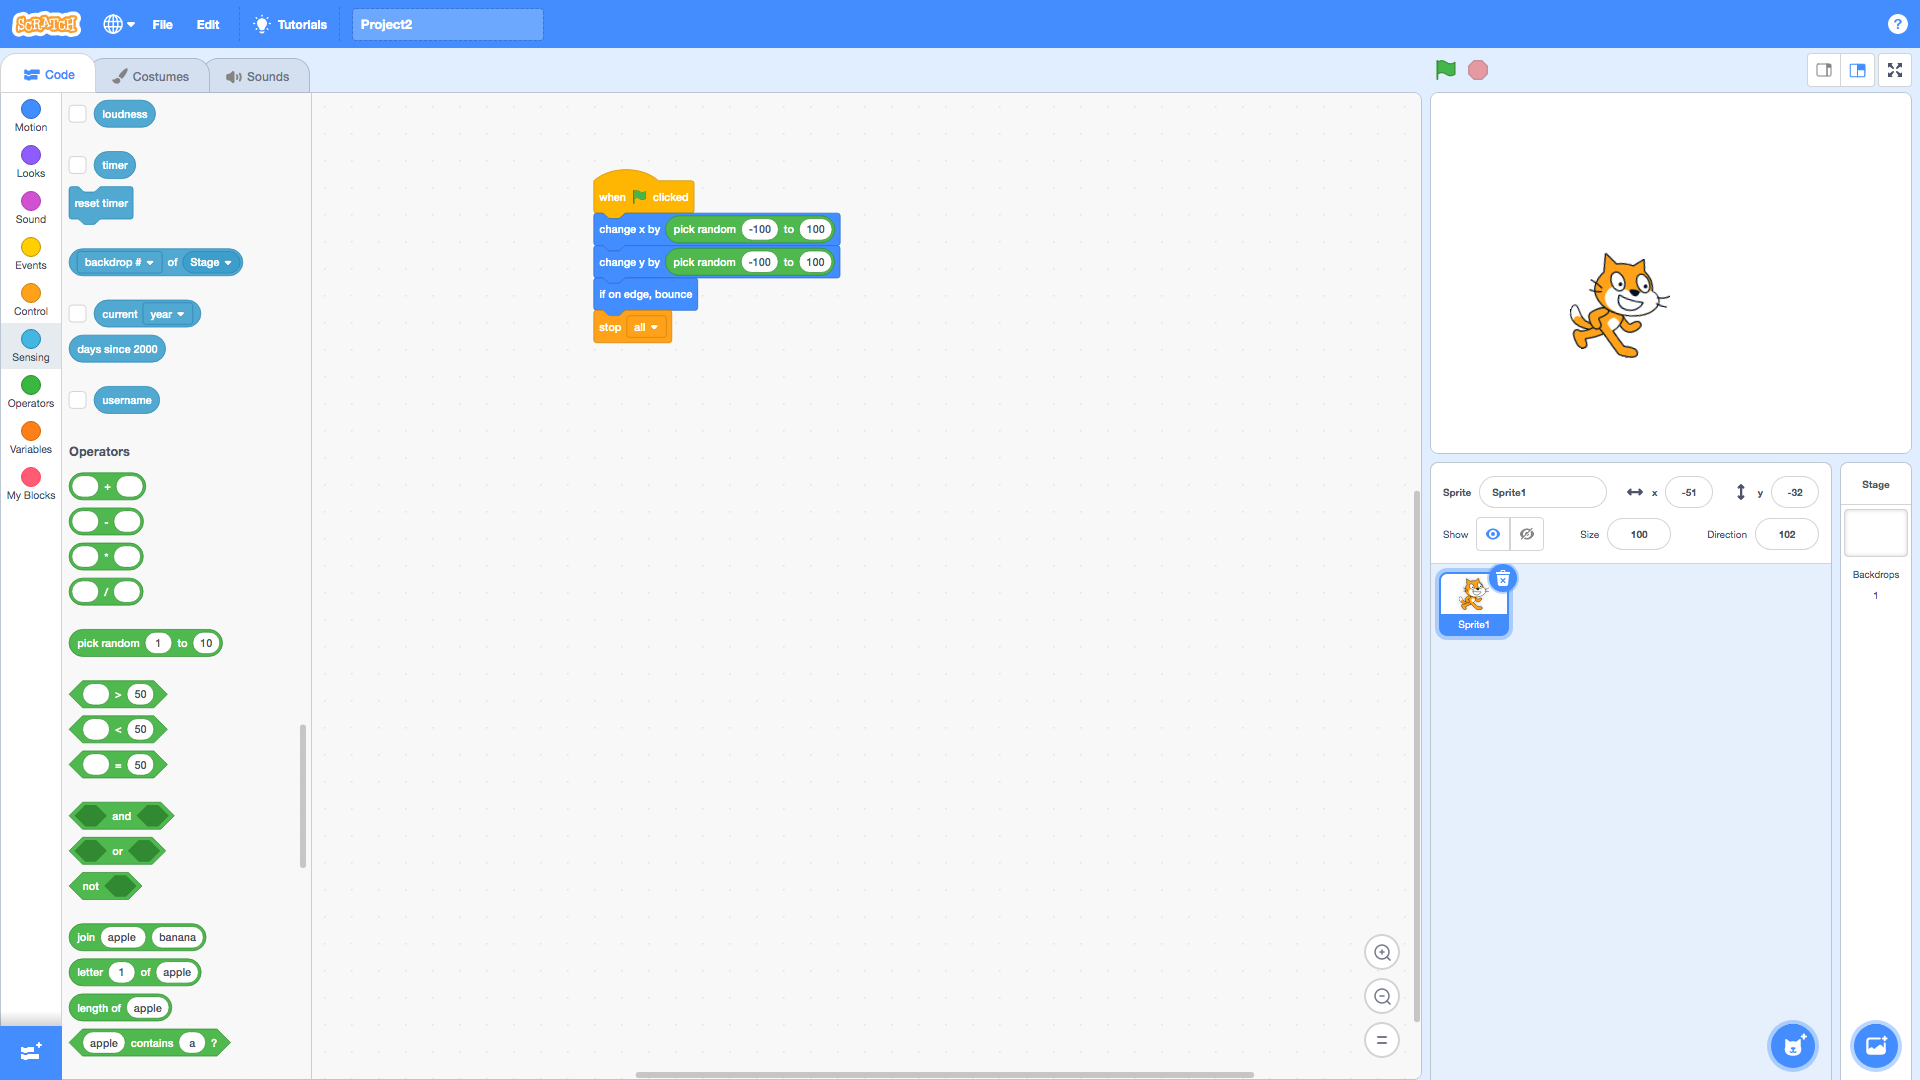
\includegraphics[width=1.0\linewidth,height=0.5\linewidth]{fig020016.png}
   \caption{Bouncing off the edges}
\label{fig020016}
\end{figure}

Next, a handy block from the group of dark orange is the block for waiting a period (Fig. \ref{fig020017}). When this block is placed between the start and end blocks, the program waits the specified number of seconds before stopping execution. During execution, it can be clearly observed that a yellow frame appears around the sequence of instructions, which symbolizes the mode of executing instructions.

\begin{figure}[H]
   \centering
   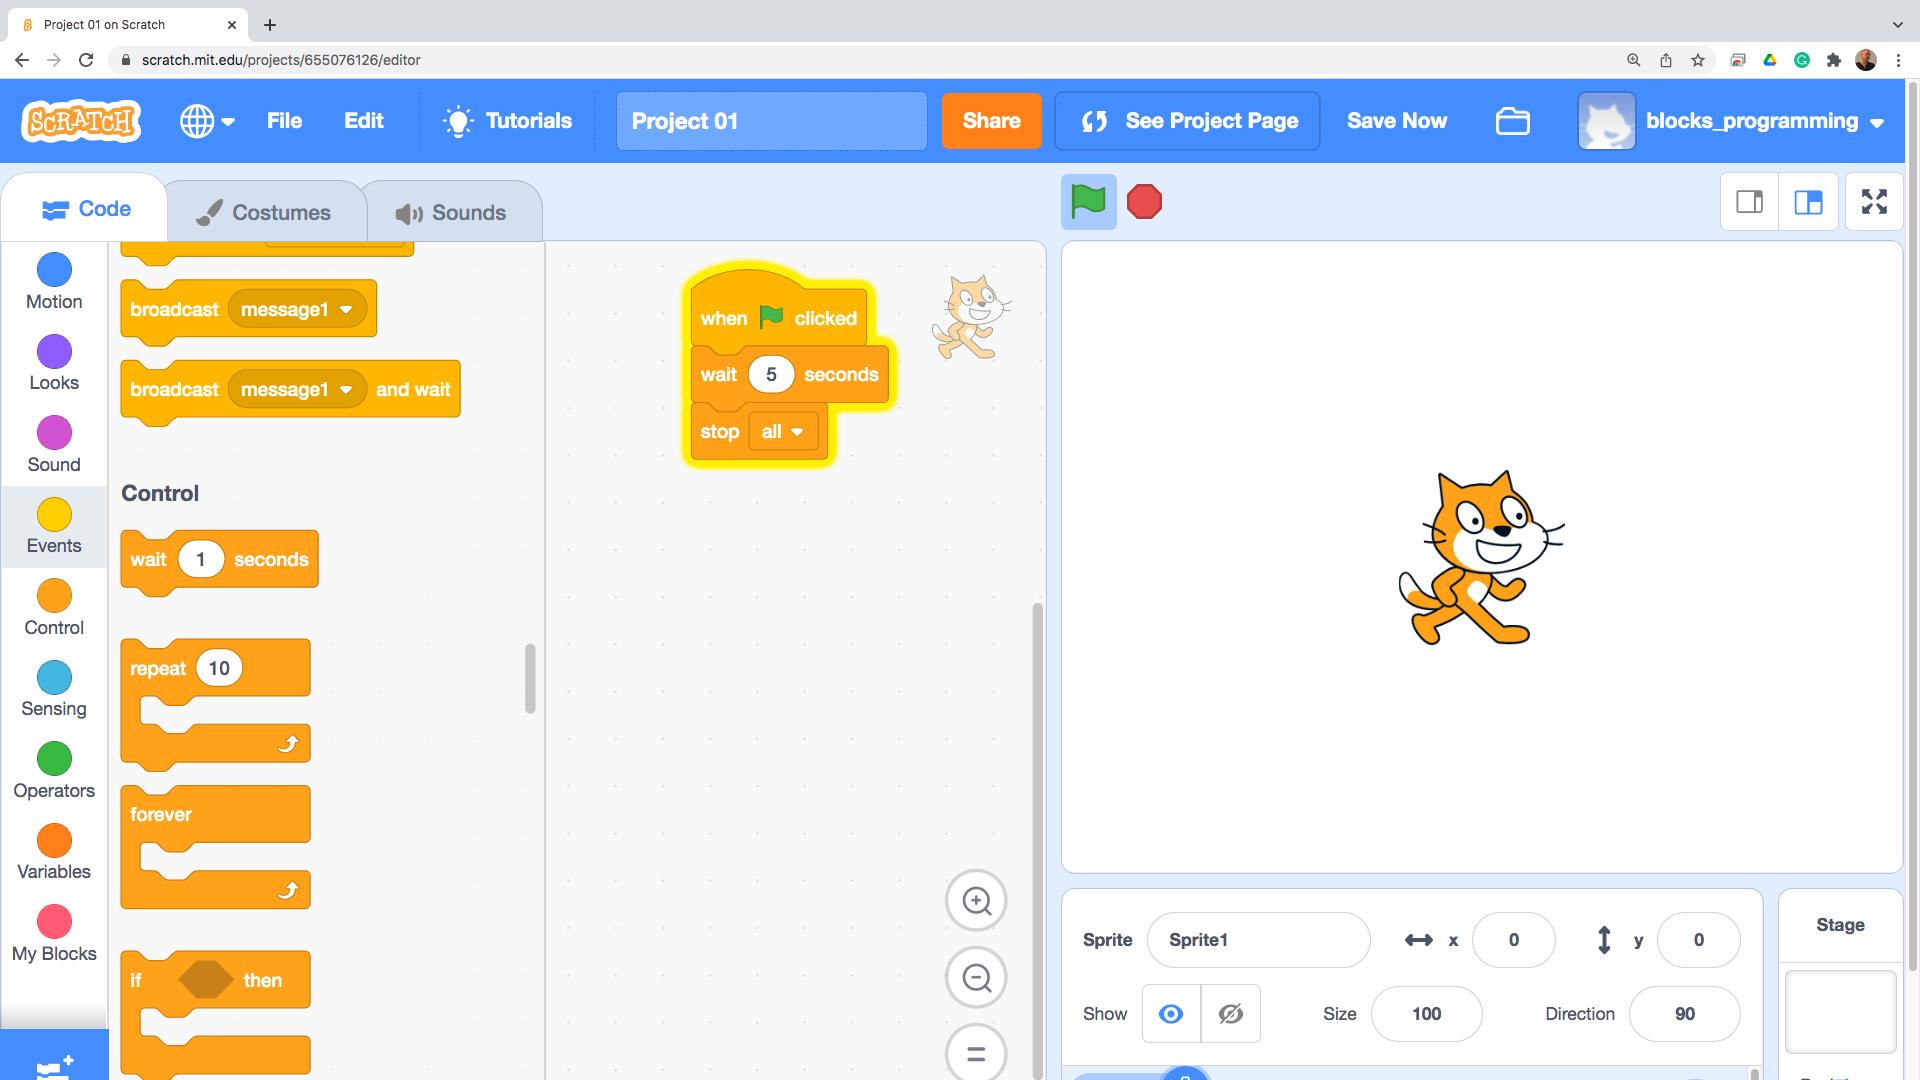
\includegraphics[width=1.0\linewidth,height=0.5\linewidth]{fig020017.png}
   \caption{Wait instruction}
\label{fig020017}
\end{figure}

The group of purple blocks contains instructions for the outer layout of the animated character. The first two blocks are intended for lines (Fig. \ref{fig020018}) that the character says (spelled as in a comic book). The first block sets the text on the screen until the next instruction. This is precisely why there needs to be a few seconds of waiting so the text remains visible to the user. The second block also has a parameter to determine how many seconds the text should be visible to the user.

\begin{figure}[H]
   \centering
   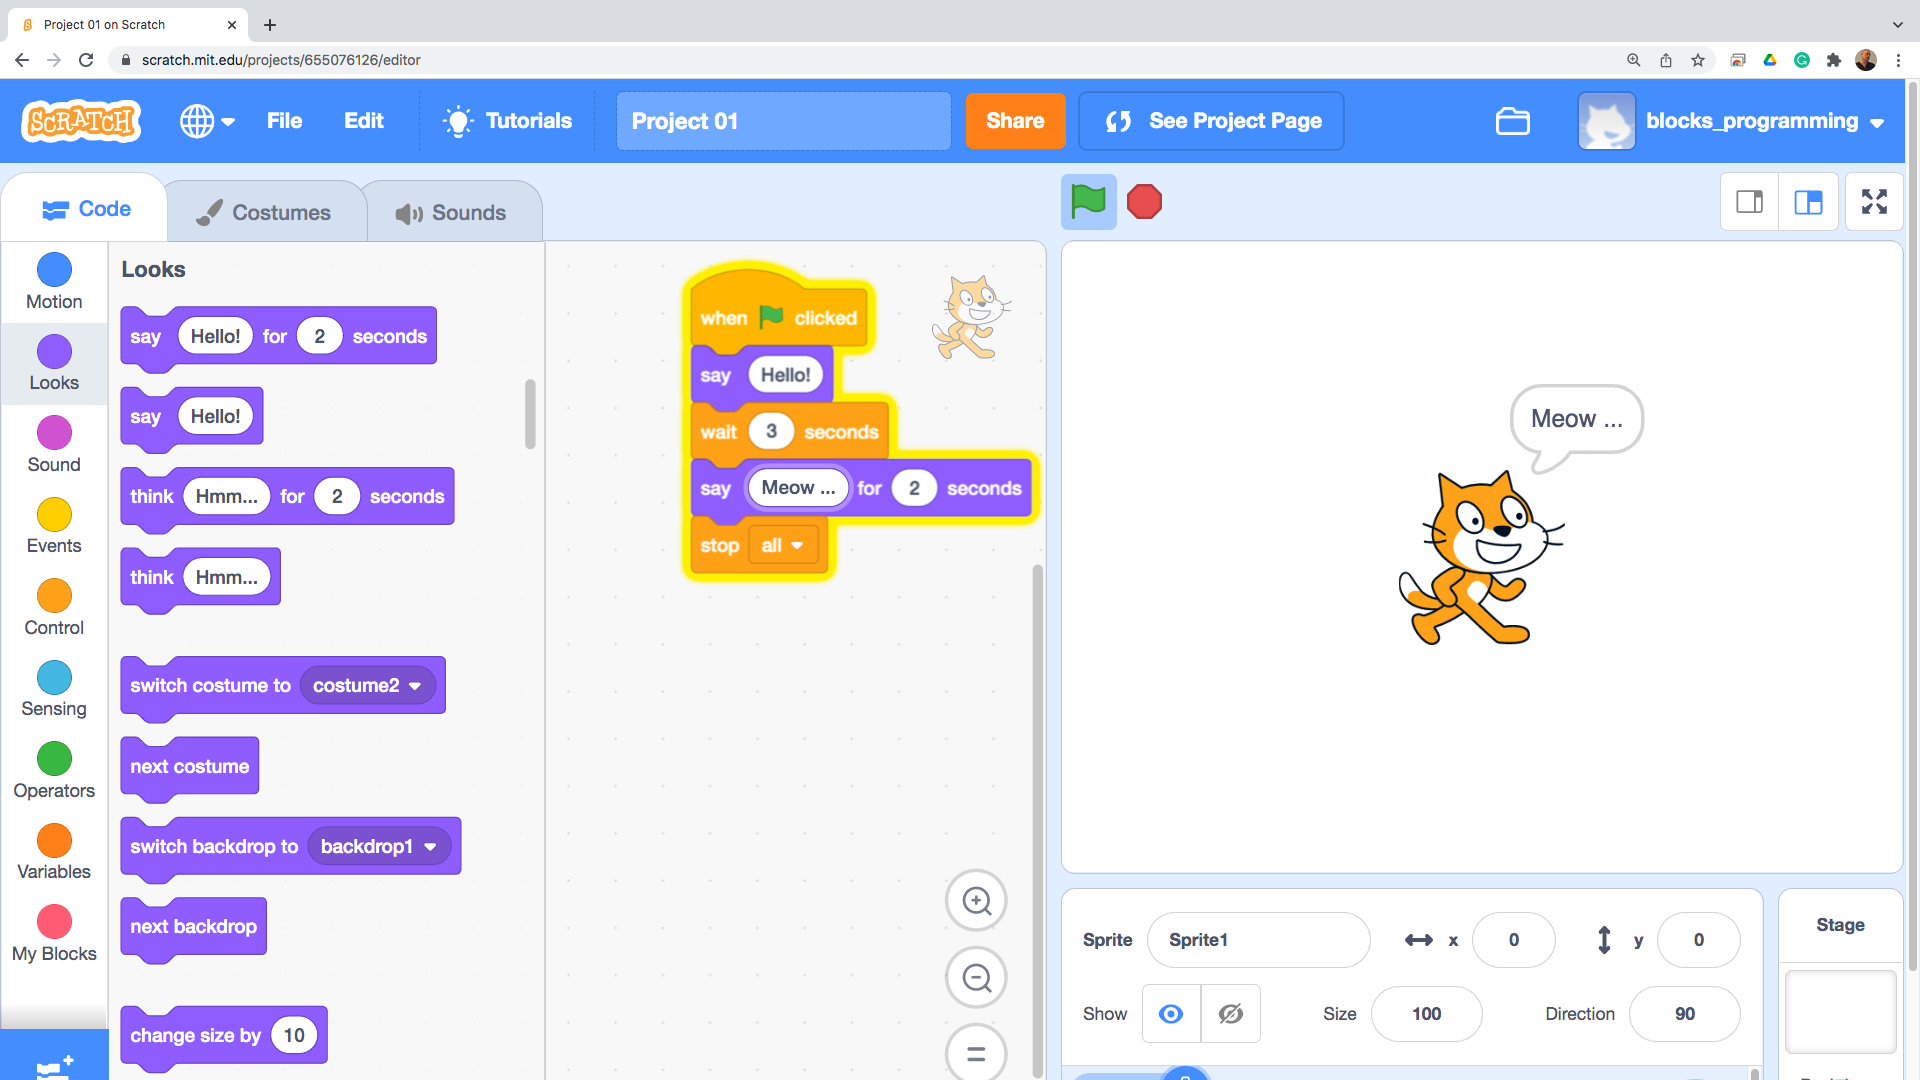
\includegraphics[width=1.0\linewidth,height=0.5\linewidth]{fig020018.png}
   \caption{Writing cues to speak}
\label{fig020018}
\end{figure}

The second two blocks are intended for lines the animated character thinks but does not say. The difference is in how the text is visualized (Fig. \ref{fig020019}).

\begin{figure}[H]
   \centering
   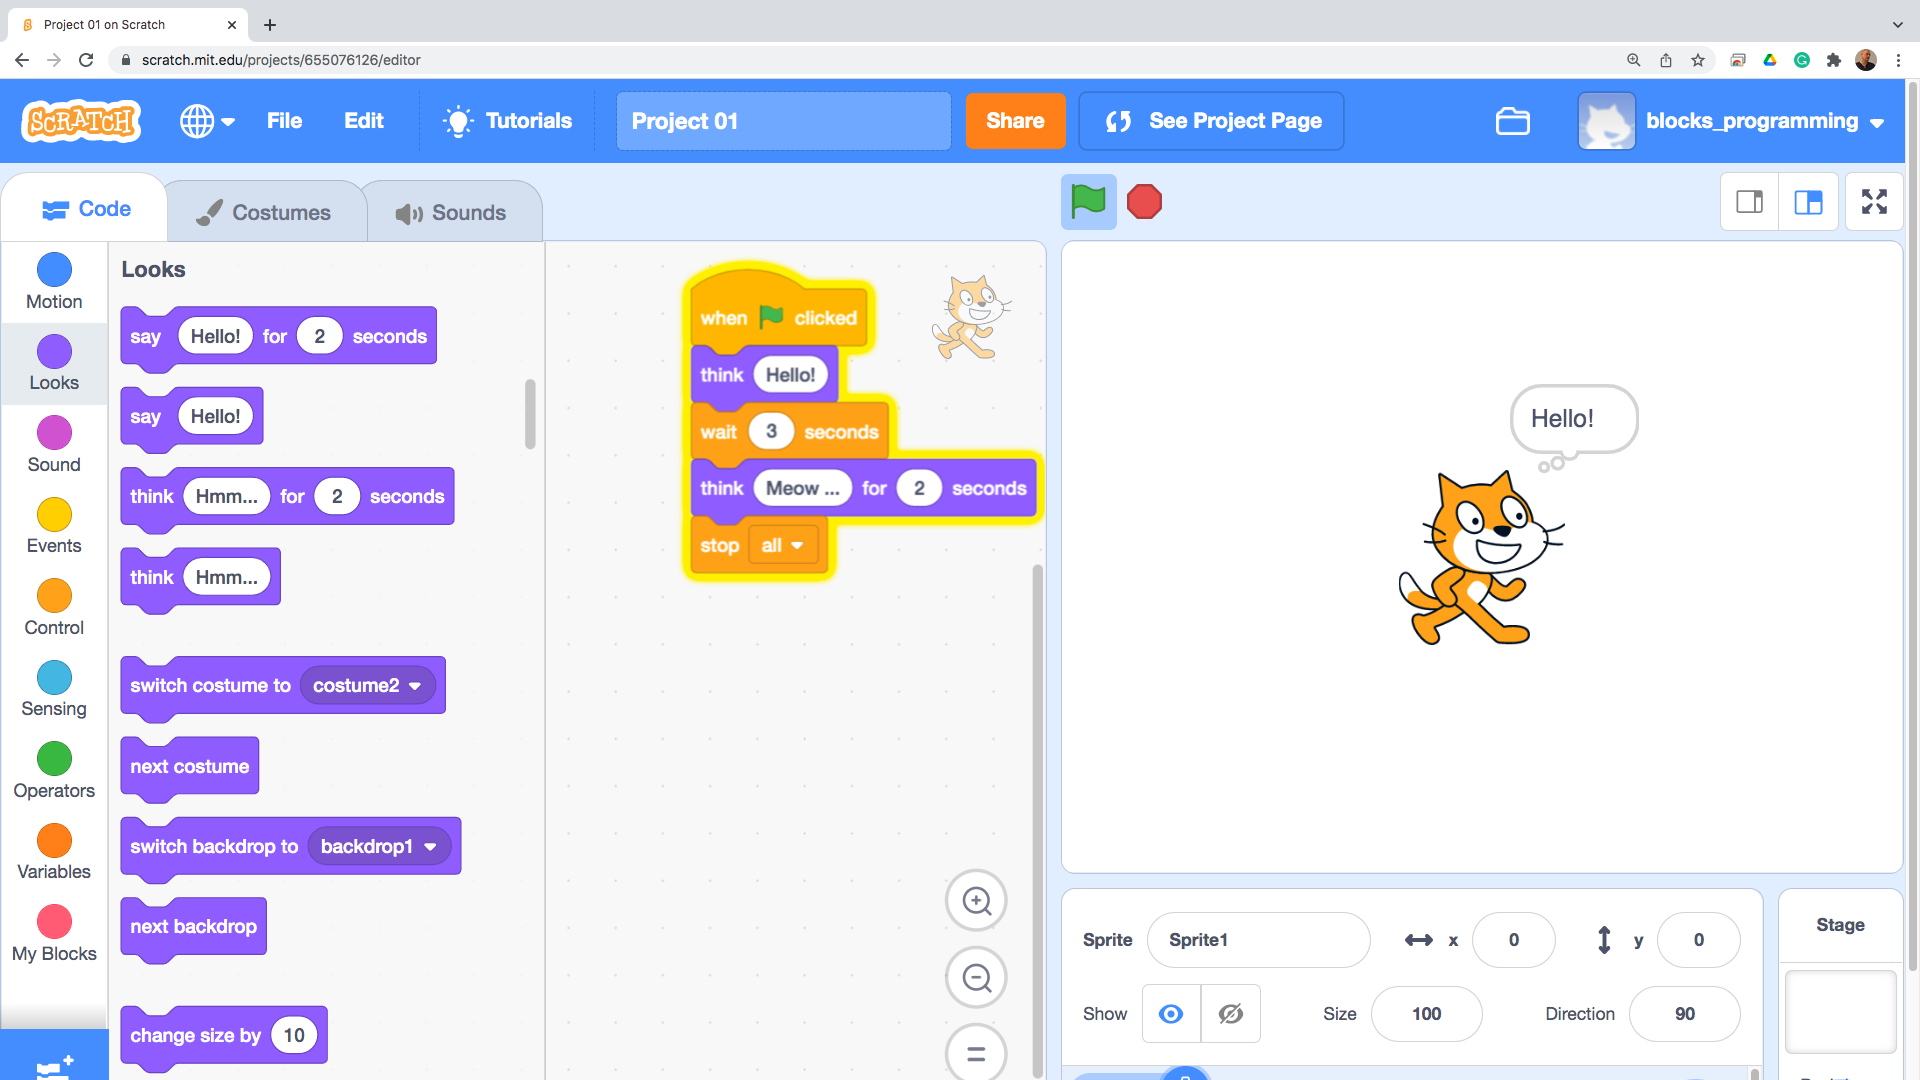
\includegraphics[width=1.0\linewidth,height=0.5\linewidth]{fig020019.png}
   \caption{Writing lines, as a thought}
\label{fig020019}
\end{figure}

Animated characters in Scratch are in the form of sprites. A sprite is a set of images of the character in different poses. Two blocks are used to change these different poses (Fig. \ref{fig020020}). The first set is a specific frame in the sprite, and the second is the next frame in the sequence.

\begin{figure}[H]
   \centering
   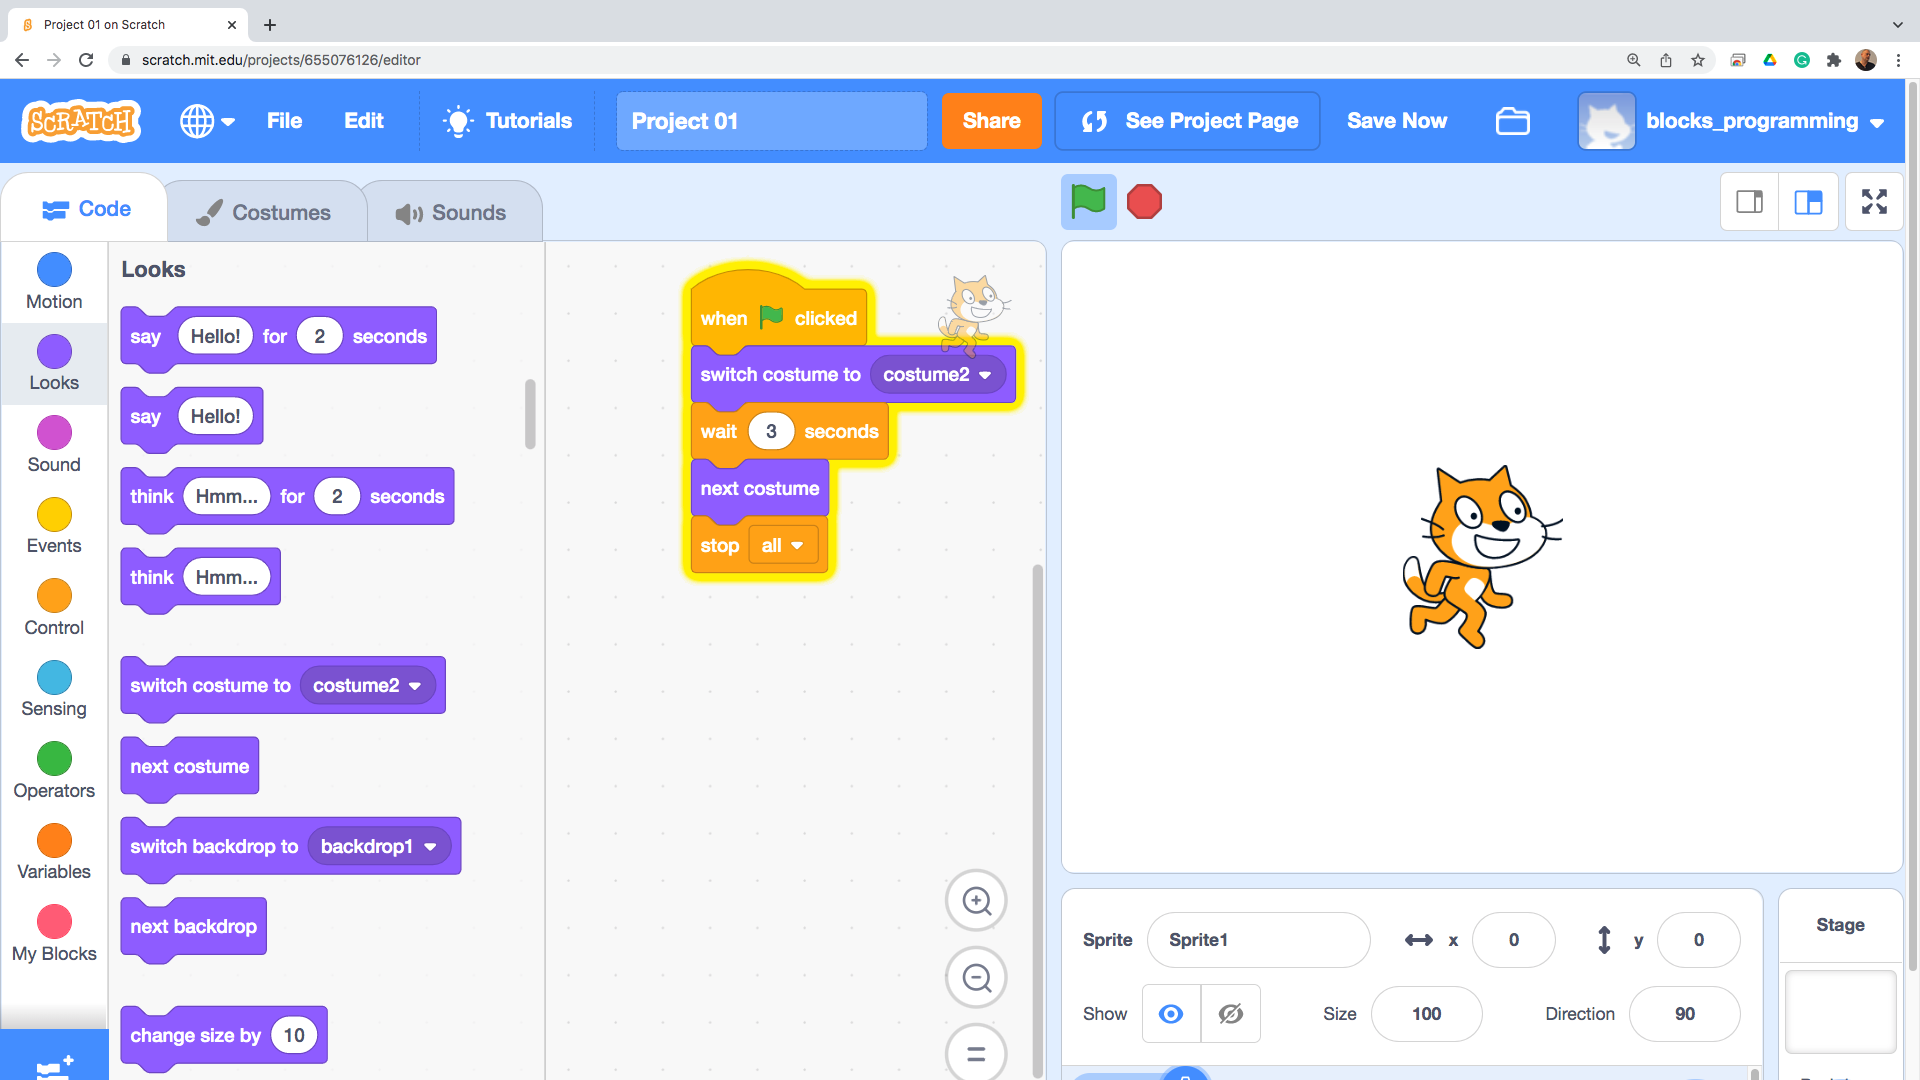
\includegraphics[width=1.0\linewidth,height=0.5\linewidth]{fig020020.png}
   \caption{Changing Poses}
\label{fig020020}
\end{figure}

In addition to the animated characters (sprites), the work scene has a background image. This background image is also subject to change, for which two separate blocks are provided (Fig. \ref{fig020021}). With the first one, background images can be selected forward, backward, randomly, or with a specific name, and with the second block, the next image in the sequence.

\begin{figure}[H]
   \centering
   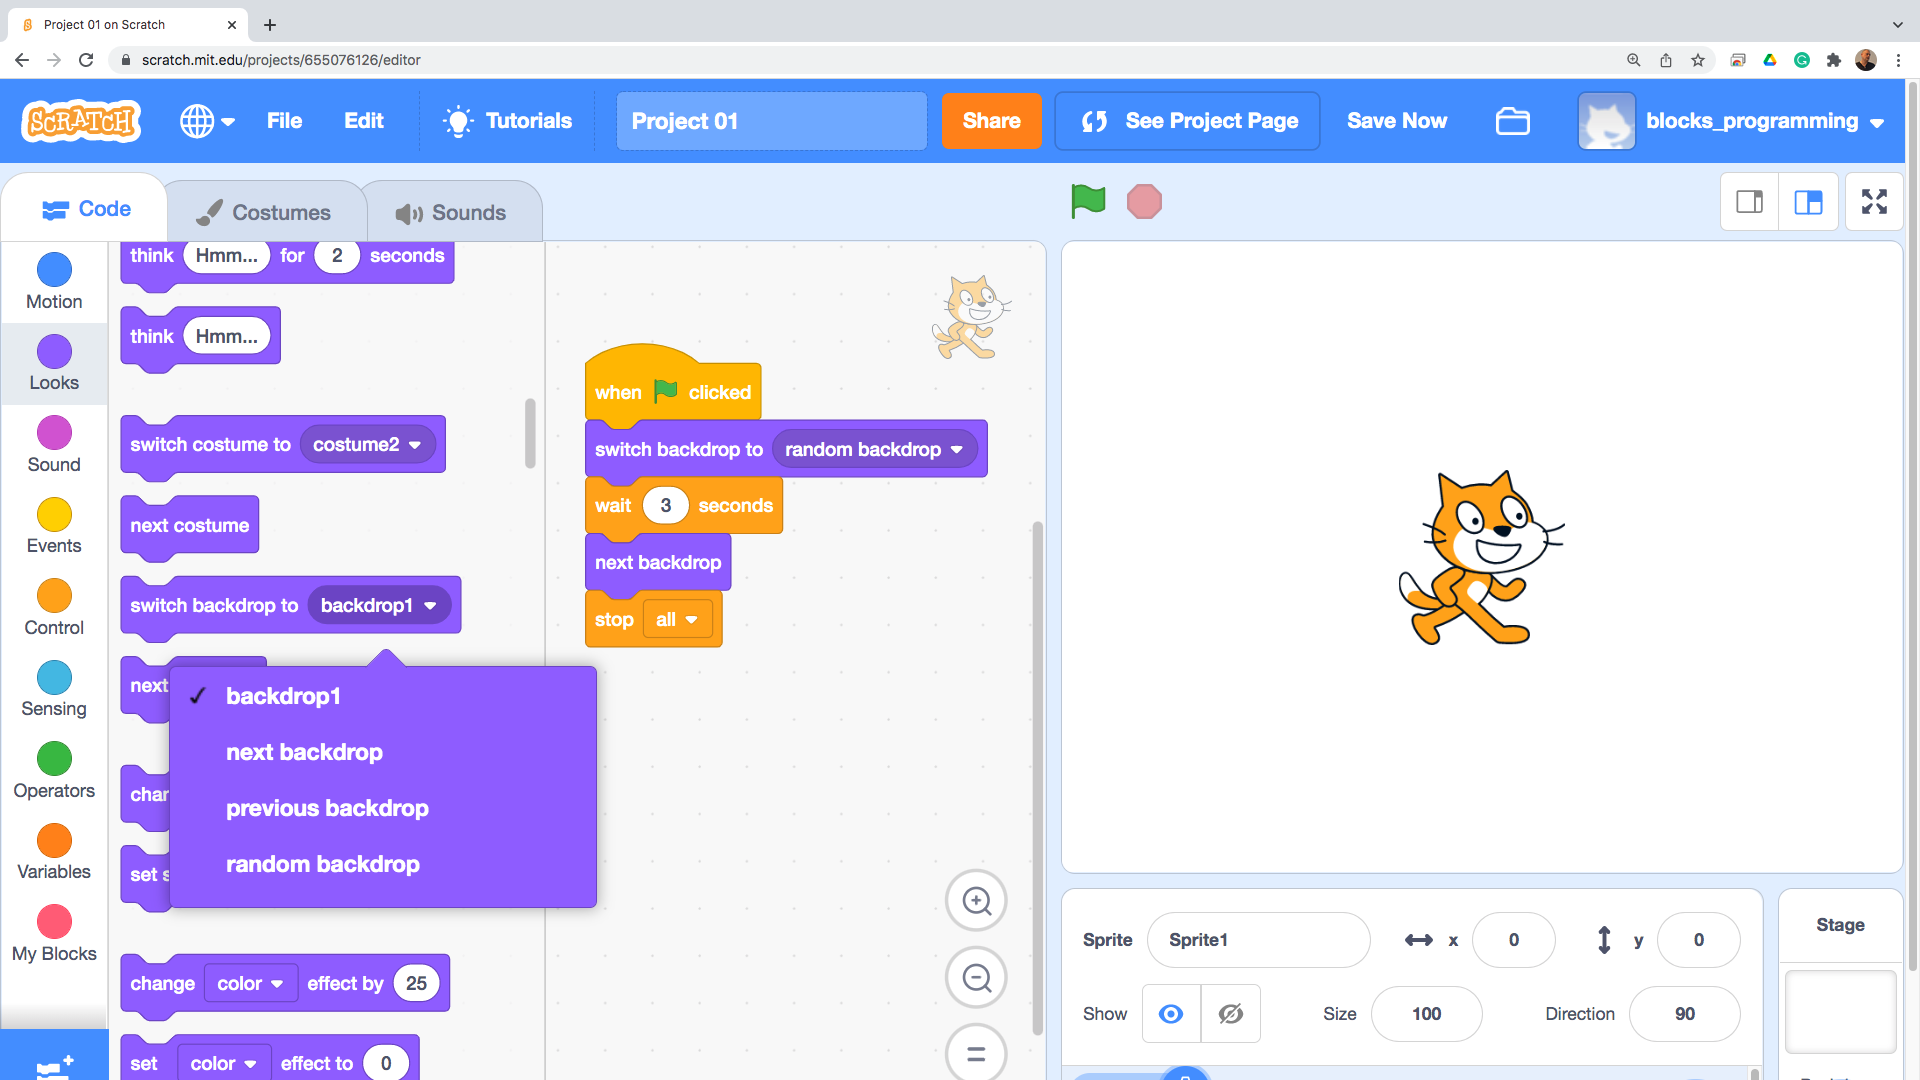
\includegraphics[width=1.0\linewidth,height=0.5\linewidth]{fig020021.png}
   \caption{Change background}
\label{fig020021}
\end{figure}

There are two specific blocks for resizing the animated character, the first resizing in absolute values and the second resizing in percentages relative to the original size (Fig. \ref{fig020022}).

\begin{figure}[H]
   \centering
   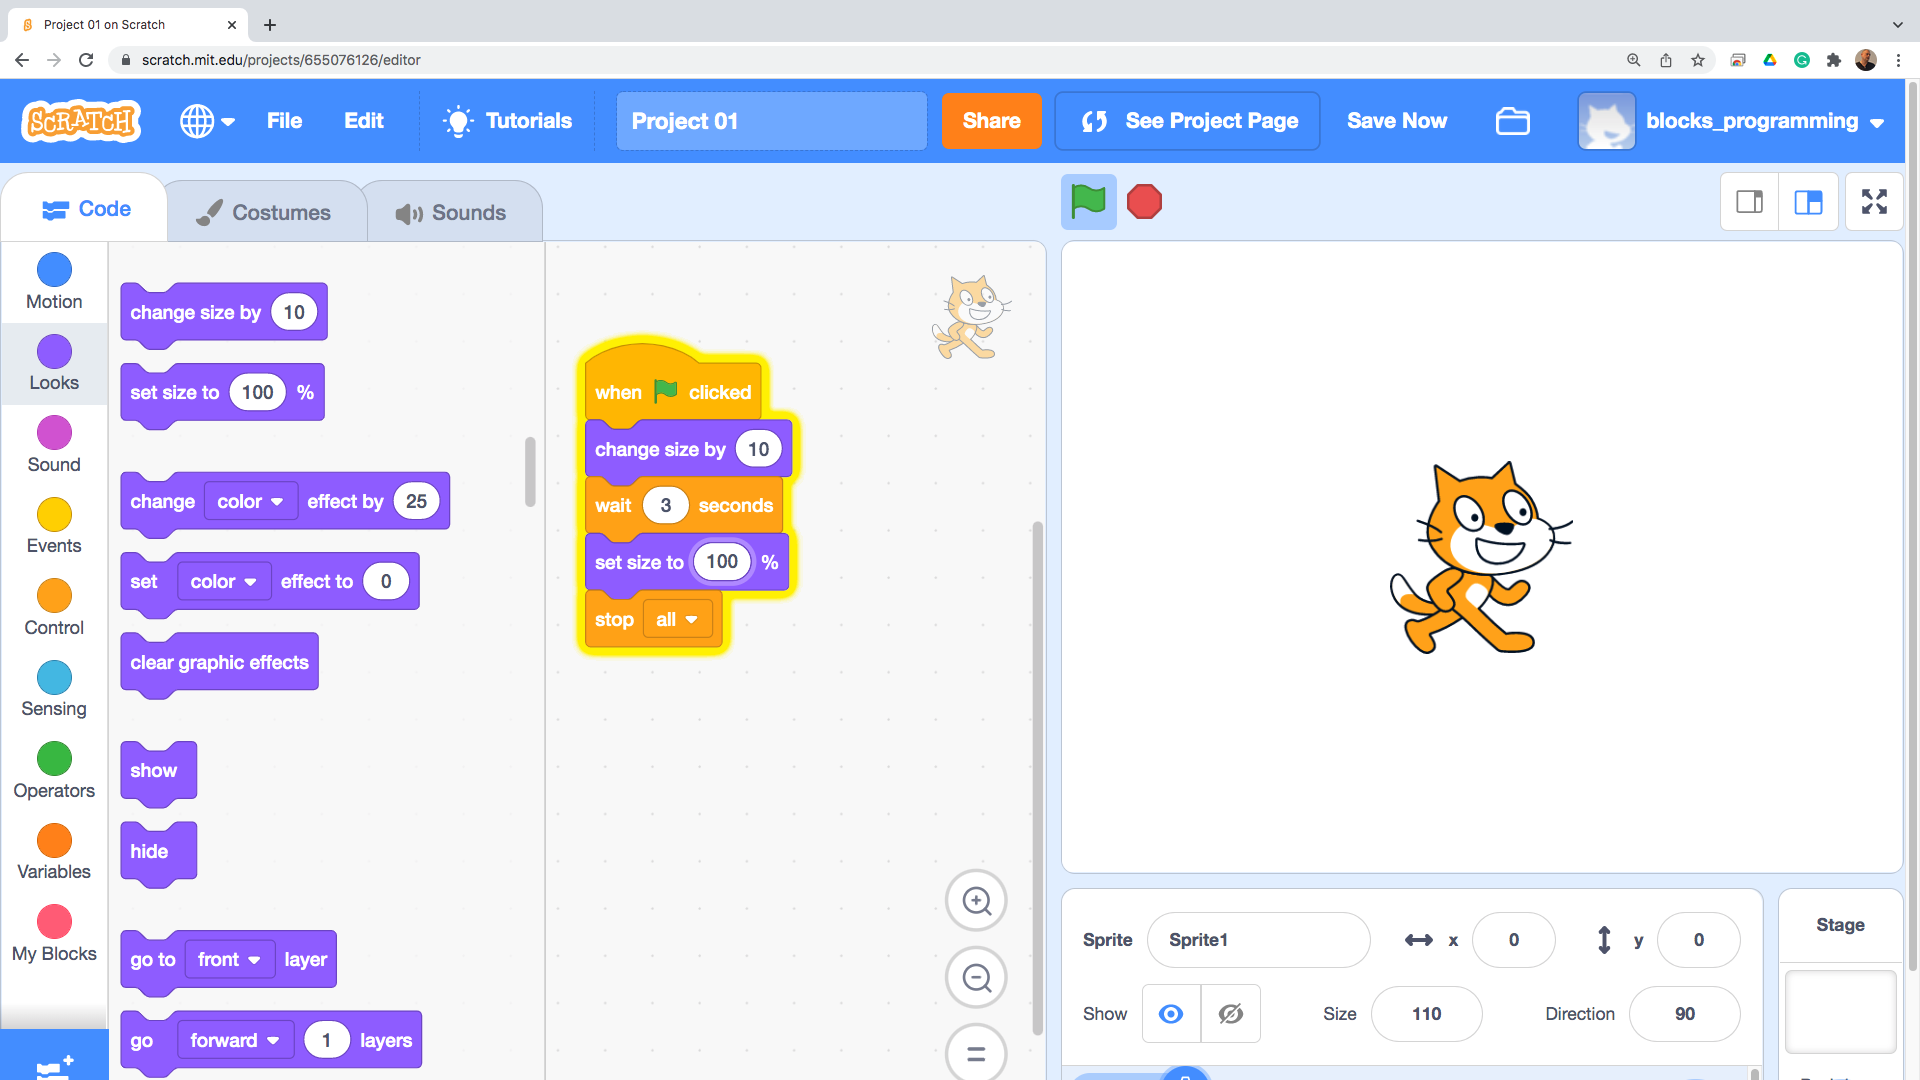
\includegraphics[width=1.0\linewidth,height=0.5\linewidth]{fig020022.png}
   \caption{Resize}
\label{fig020022}
\end{figure}

Three blocks are provided for changing the visual layout of the animated character (Fig. \ref{fig020023}). The first two set a change, which can be in color, various distortions, pixelation, mosaic, transparency, or brightness, and the third block cancels any decorations made. The first block causes a relative change to the character's current state, and the second block sets a fundamental change. Again, giving it a few seconds is essential so that the changes are clearly discernible.

\begin{figure}[H]
   \centering
   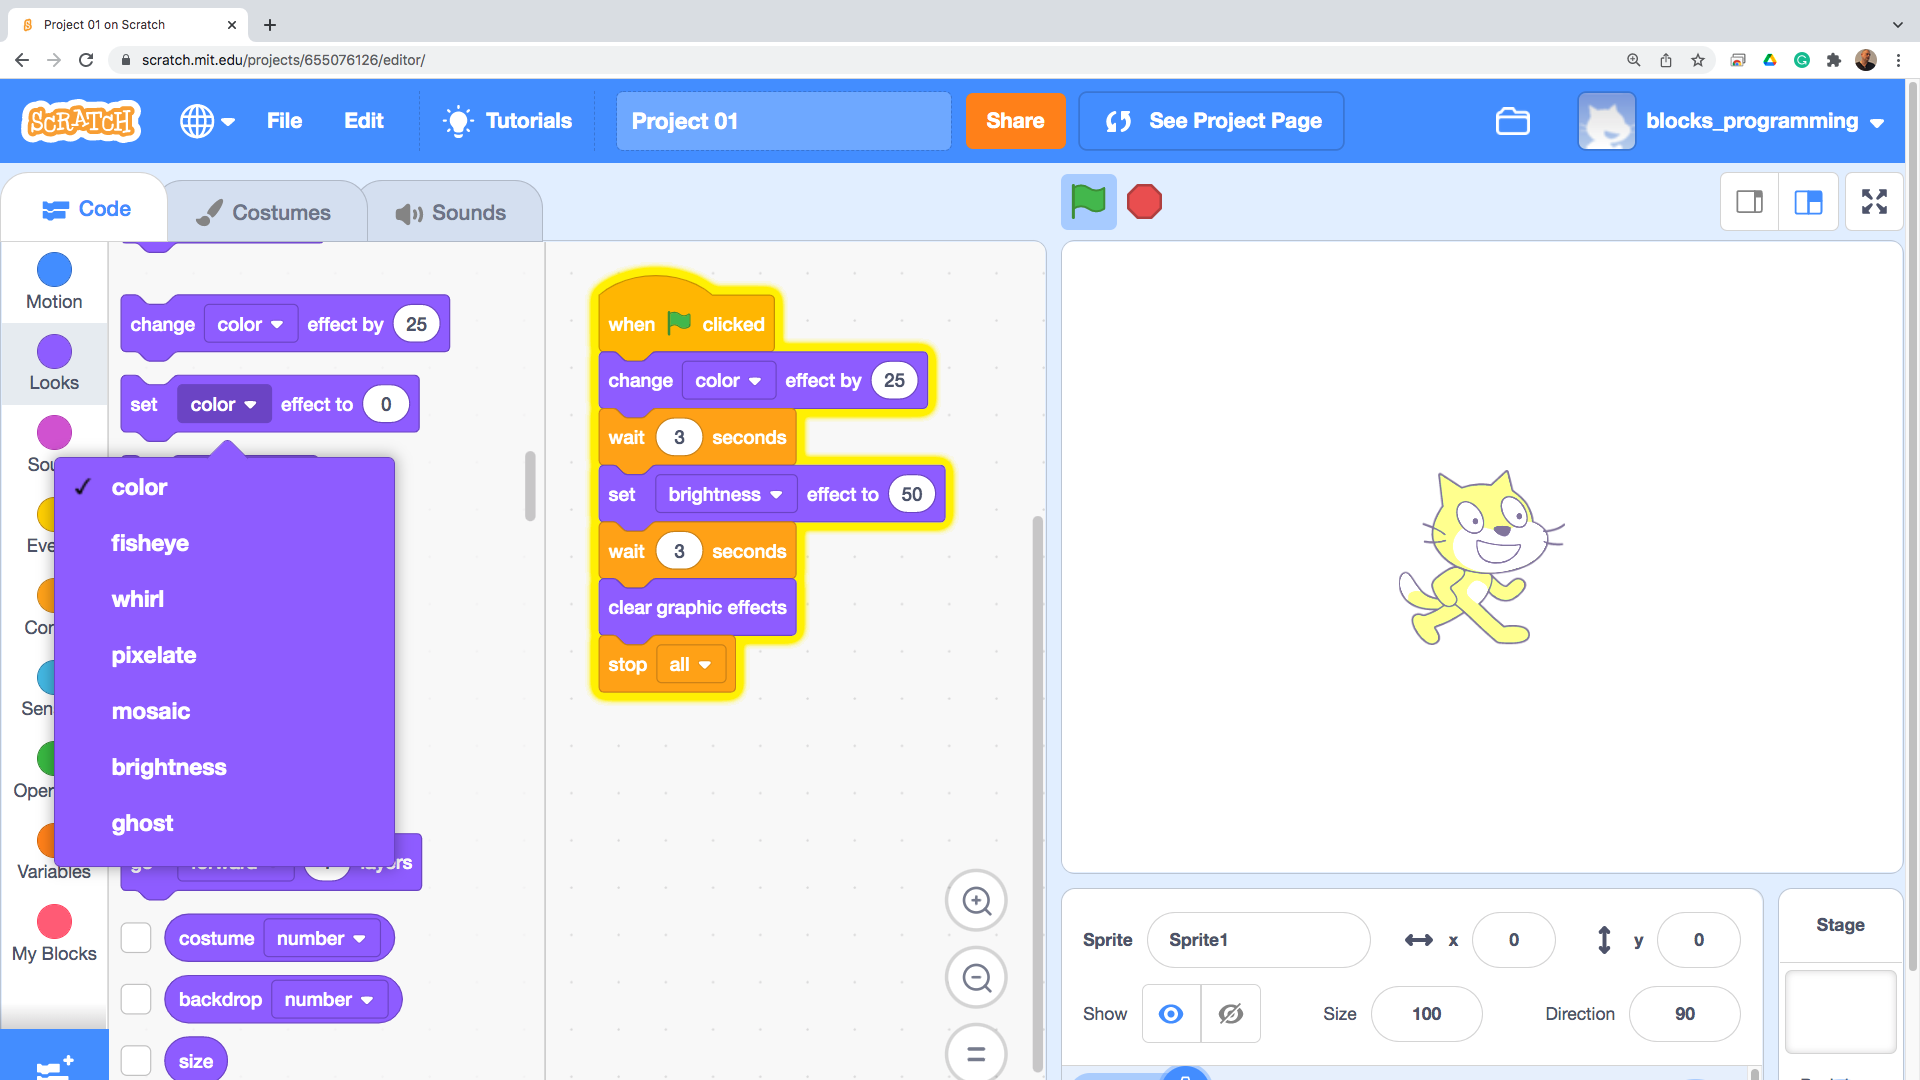
\includegraphics[width=1.0\linewidth,height=0.5\linewidth]{fig020023.png}
   \caption{Change appearance}
\label{fig020023}
\end{figure}

Working with sprites is primarily for achieving animated effects. The different animated characters in the scene have specific interactions with each other. The script of the developed project determines at what moment each of the characters appears on the scene and at what moment they disappear. Two blocks performing these actions are provided to carry out the appearance and disappearance (Fig. \ref{fig020024}).

\begin{figure}[H]
   \centering
   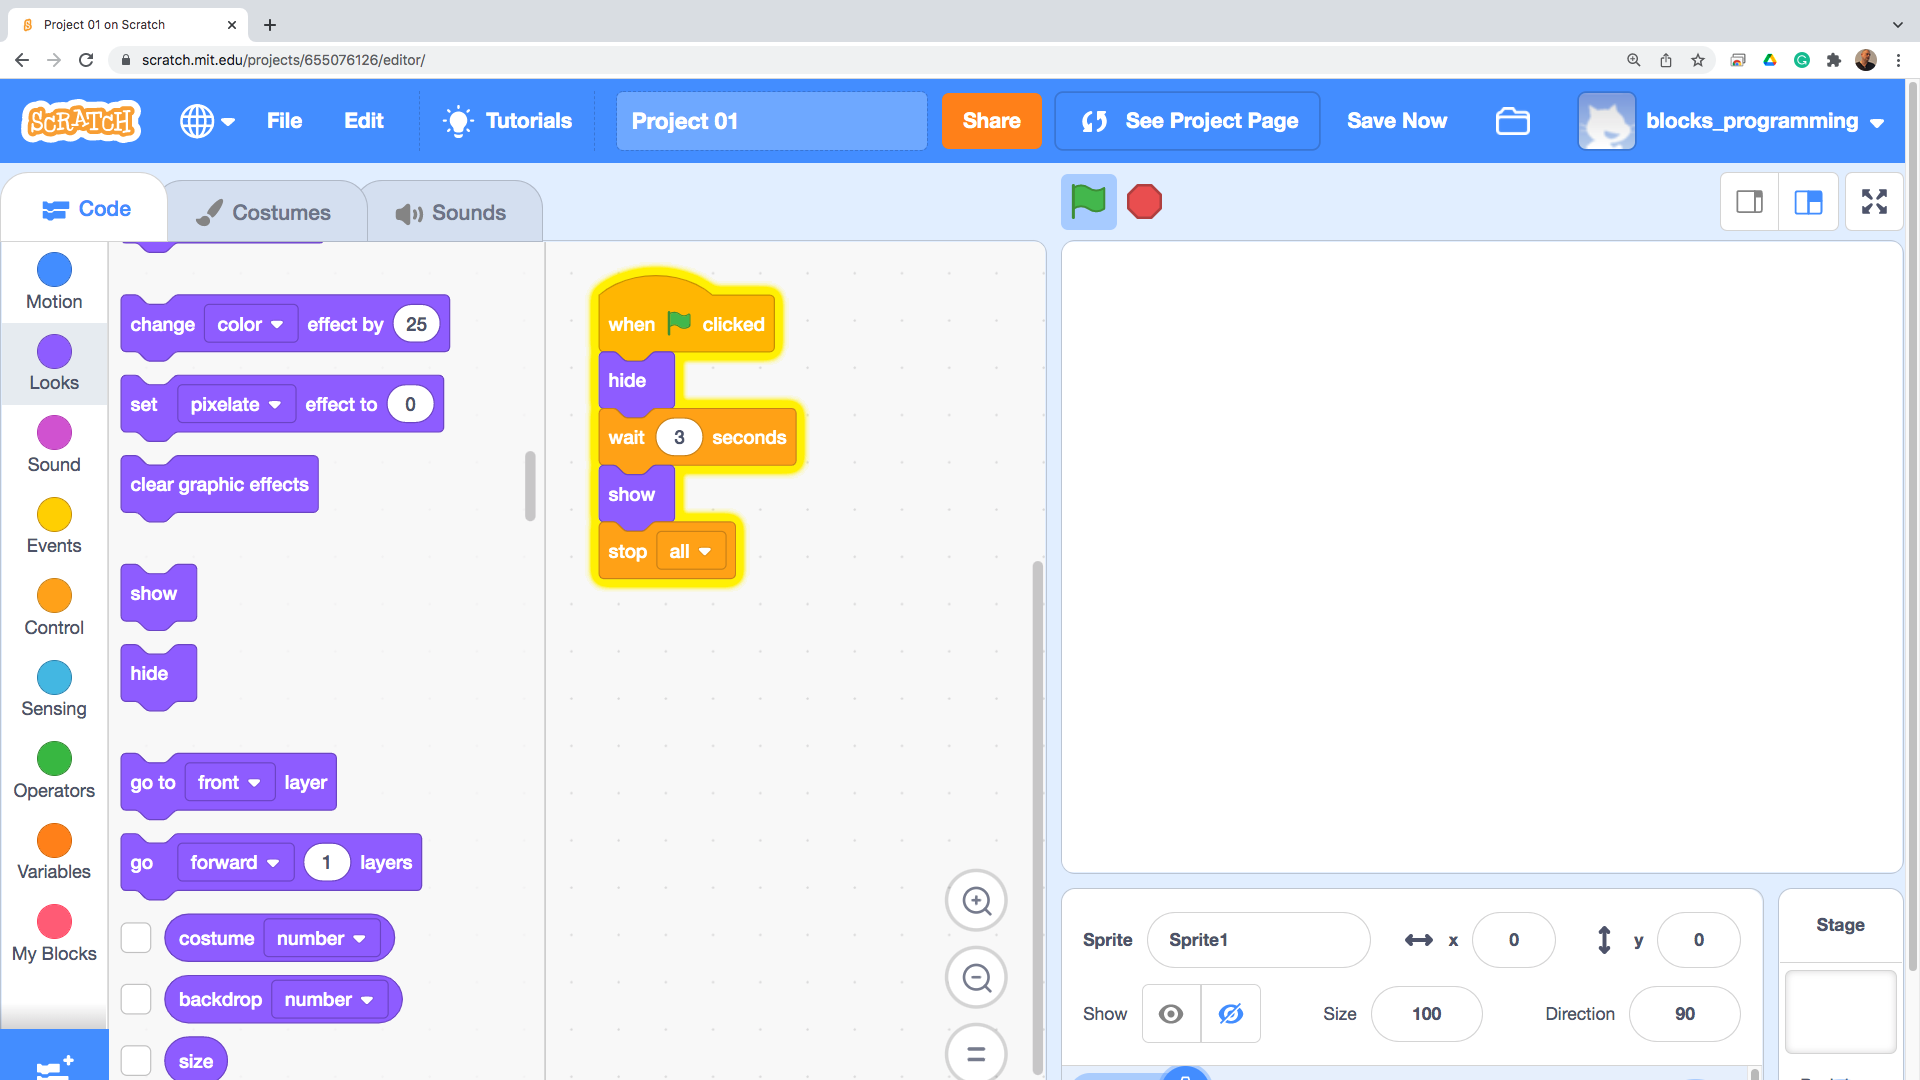
\includegraphics[width=1.0\linewidth,height=0.5\linewidth]{fig020024.png}
   \caption{Hide and show}
\label{fig020024}
\end{figure}

Many bitmap software products organize different images into layers. Examples are Adobe Photoshop, GIMP, Microsoft Word, and LibreOffice Draw. The layered organization is logical, as different sprites can overlap at specific points in time. In some of the graphics software packages, layers are perceived as a Z-buffer. In Scratch, the ability to work with layers is also available, with two specific blocks allowing the sprite to move forward and backward through the layers (Fig. \ref{fig020025}).

\begin{figure}[H]
   \centering
   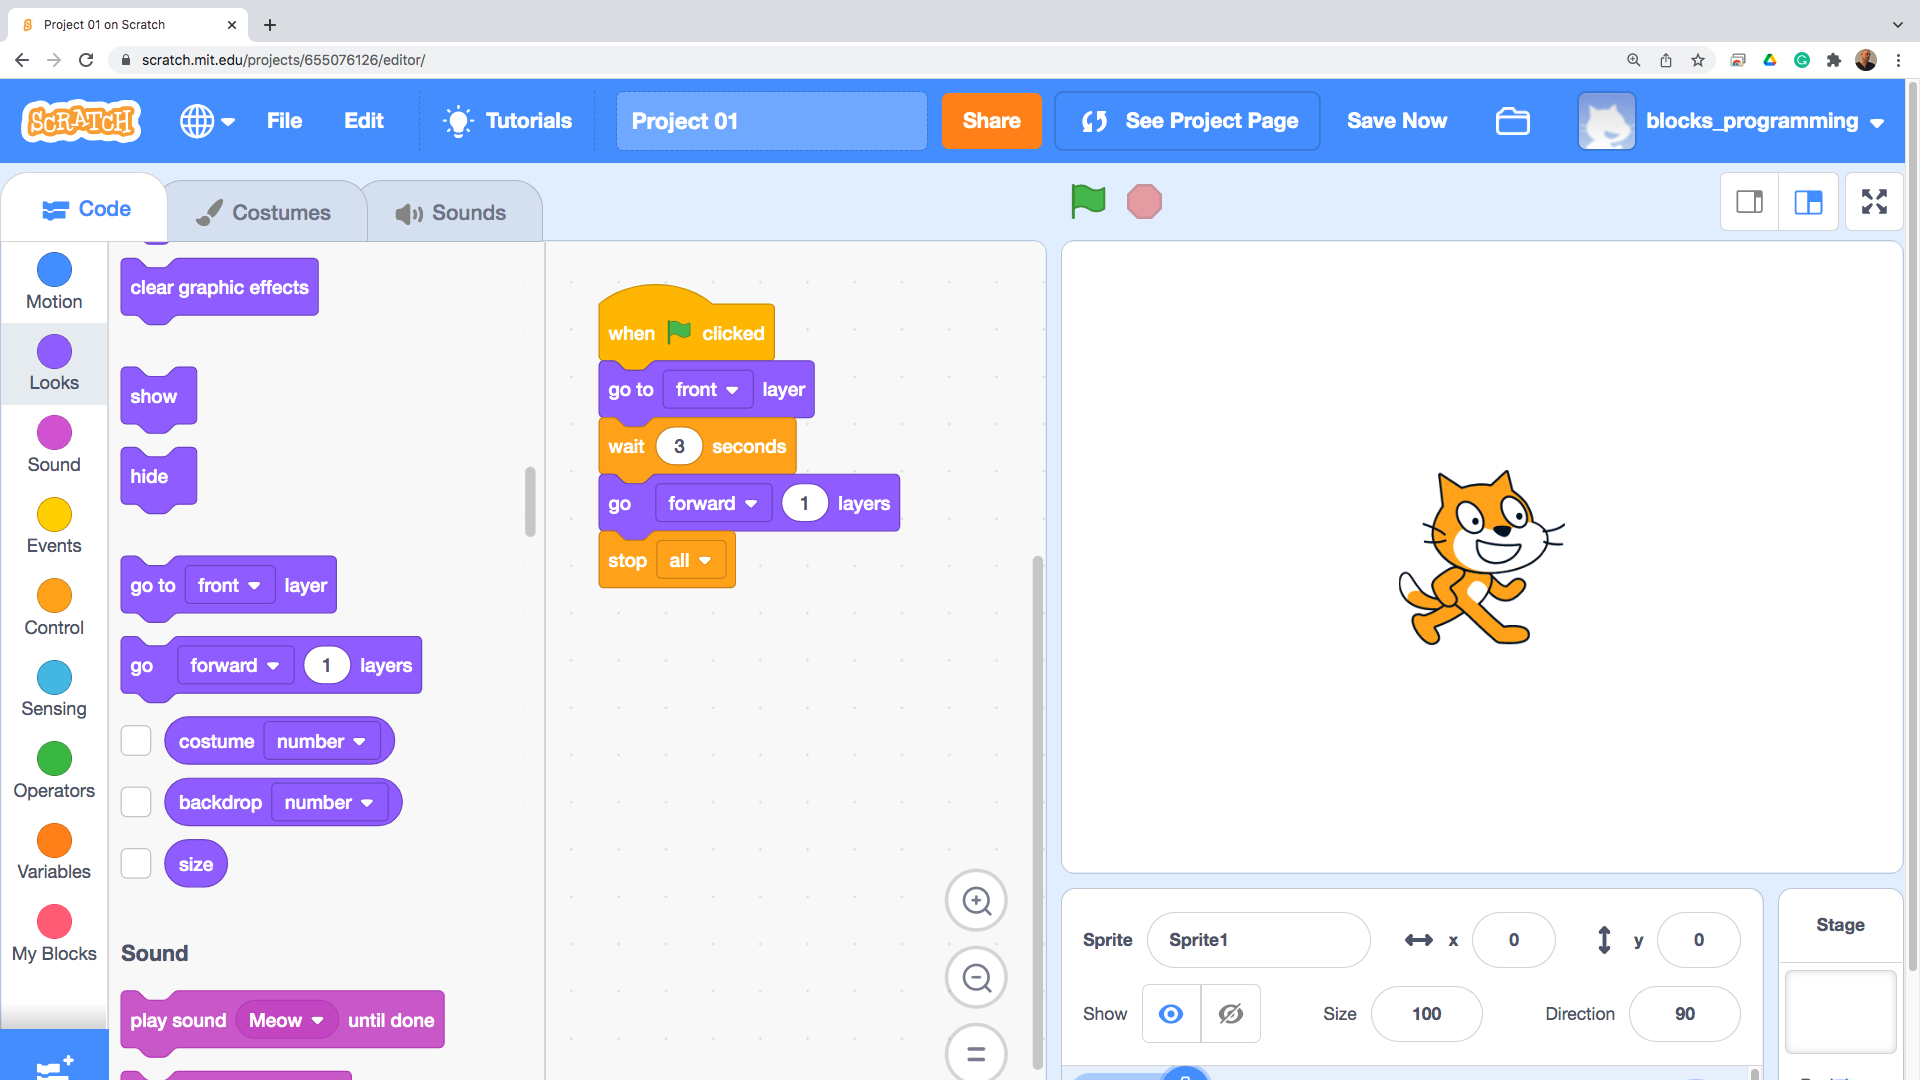
\includegraphics[width=1.0\linewidth,height=0.5\linewidth]{fig020025.png}
   \caption{Navigation through layers}
\label{fig020025}
\end{figure}

The group of blocks in magenta is for sound layout. The performance of sounds is achieved with the first two blocks in the group (Fig. \ref{fig020026}). The first block plays the sound until it is finished, and the second block starts it and passes the playback to the next block. With the third block, all playing sounds are stopped. The software environment also allows sounds to be recorded from the user's computer.

\begin{figure}[H]
   \centering
   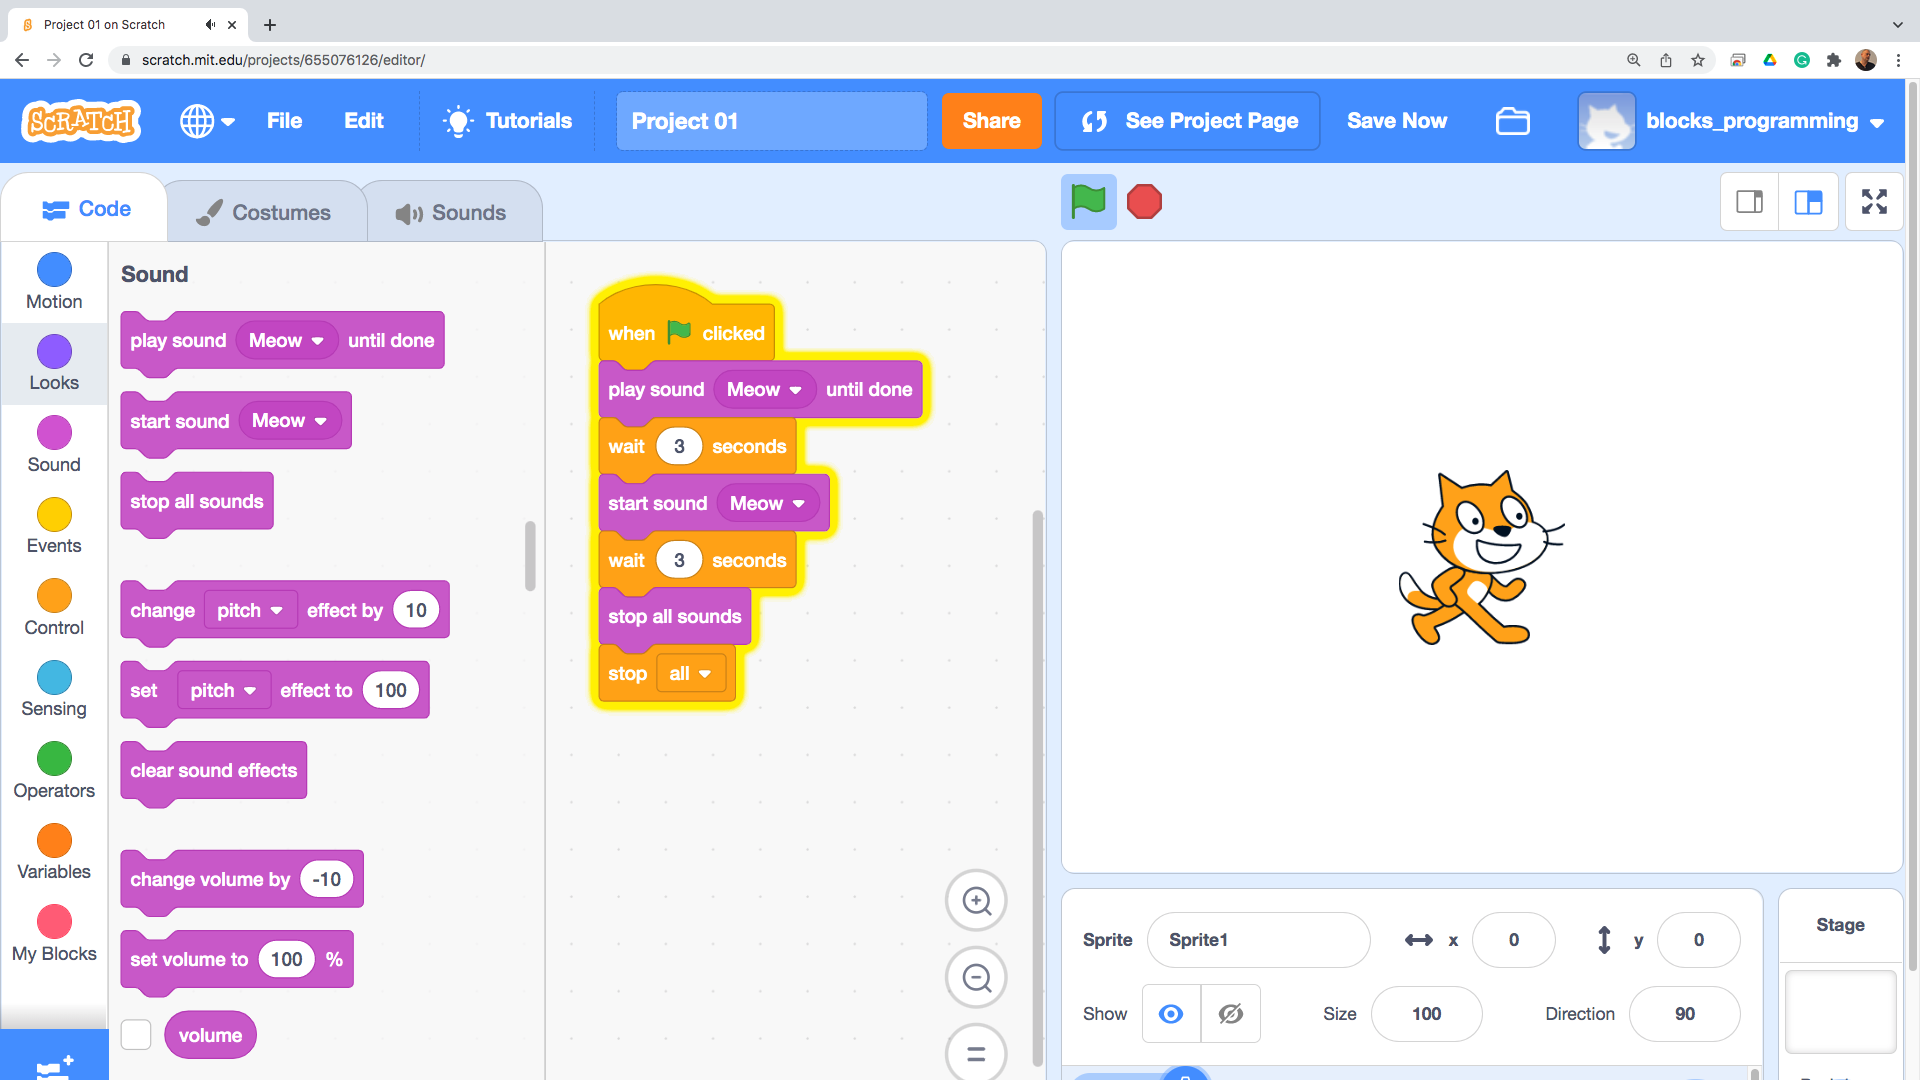
\includegraphics[width=1.0\linewidth,height=0.5\linewidth]{fig020026.png}
   \caption{Playing Sounds}
\label{fig020026}
\end{figure}

The pitch (frequency) and stereo (left/right) blocks can change two of the sounds' characteristics. Both blocks have numerical values for the specified characteristics (Fig. \ref{fig020027}).

\begin{figure}[H]
   \centering
   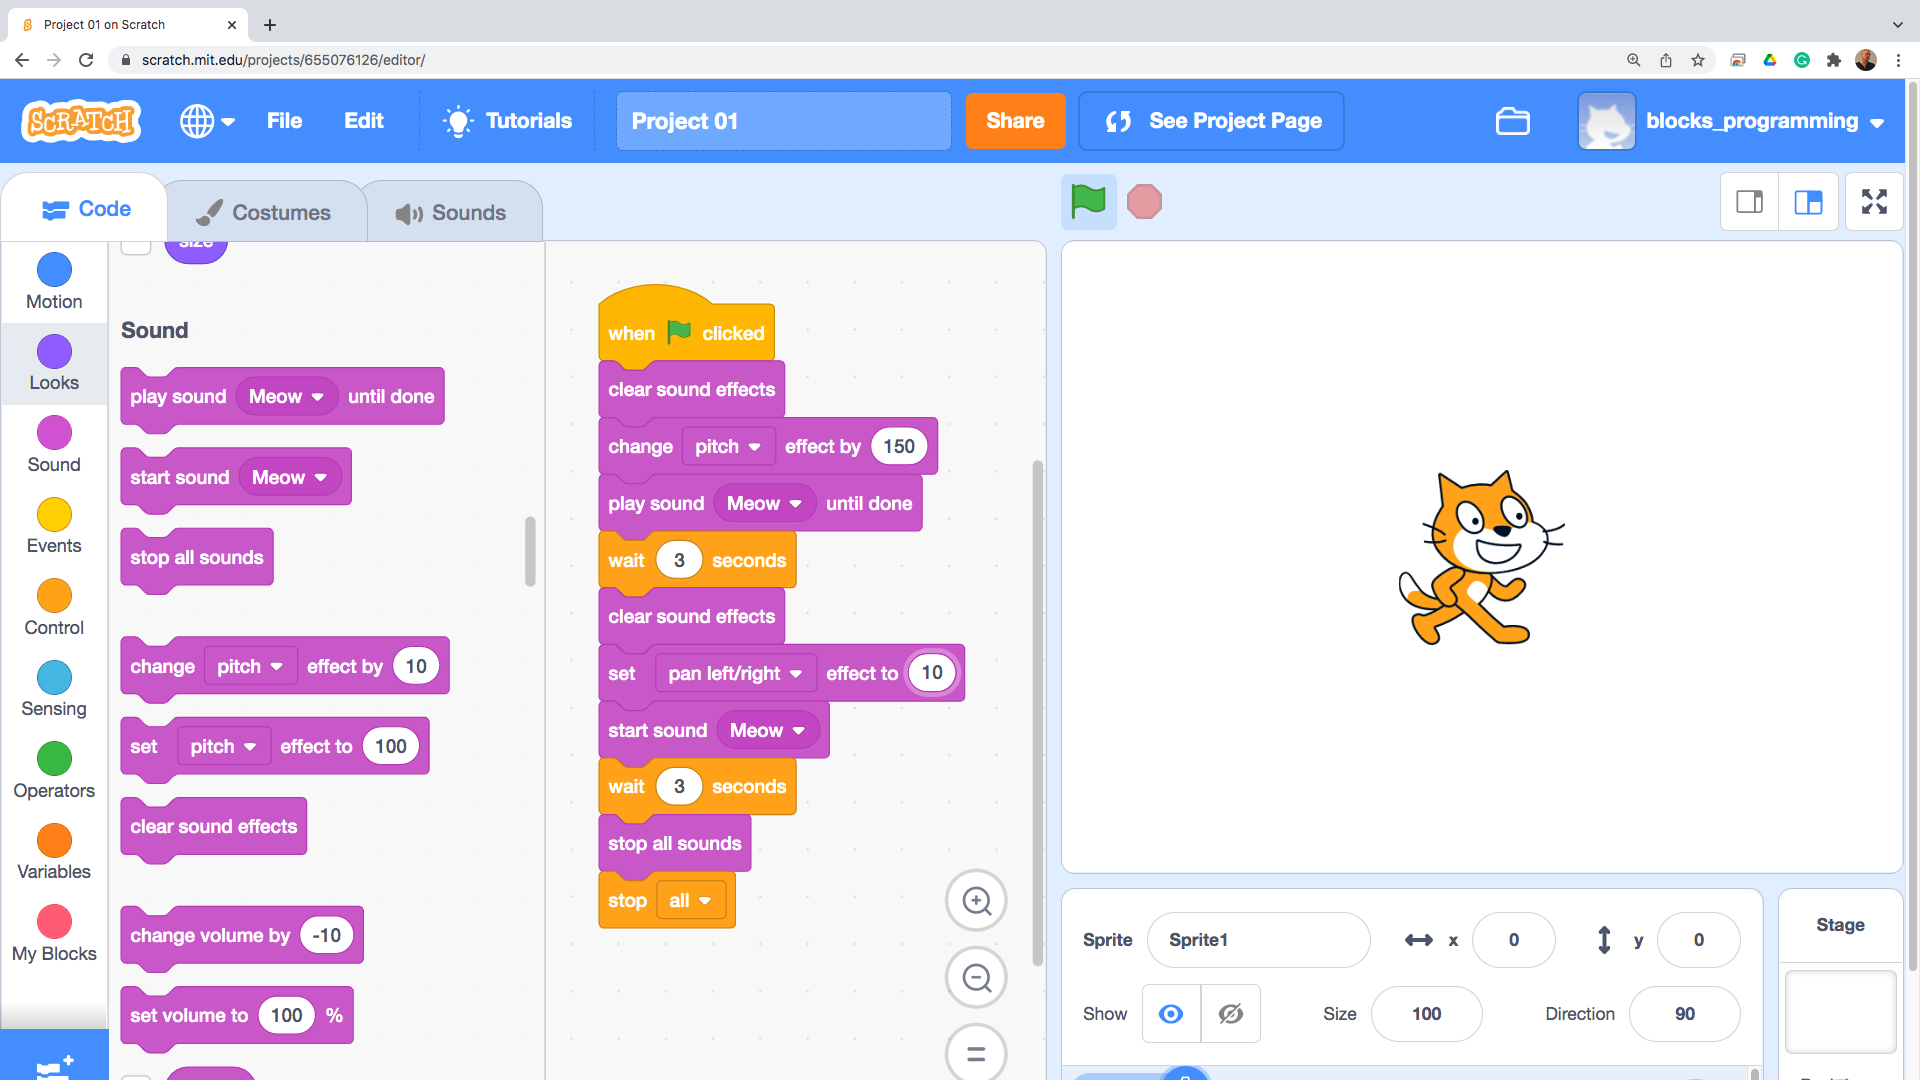
\includegraphics[width=1.0\linewidth,height=0.5\linewidth]{fig020027.png}
   \caption{Sound Characteristics}
\label{fig020027}
\end{figure}

To achieve a richer sound picture, the strength of the different sounds can be controlled with two blocks (Fig. \ref{fig020028}). The former controls volume in absolute value, the latter as percentages.

\begin{figure}[H]
   \centering
   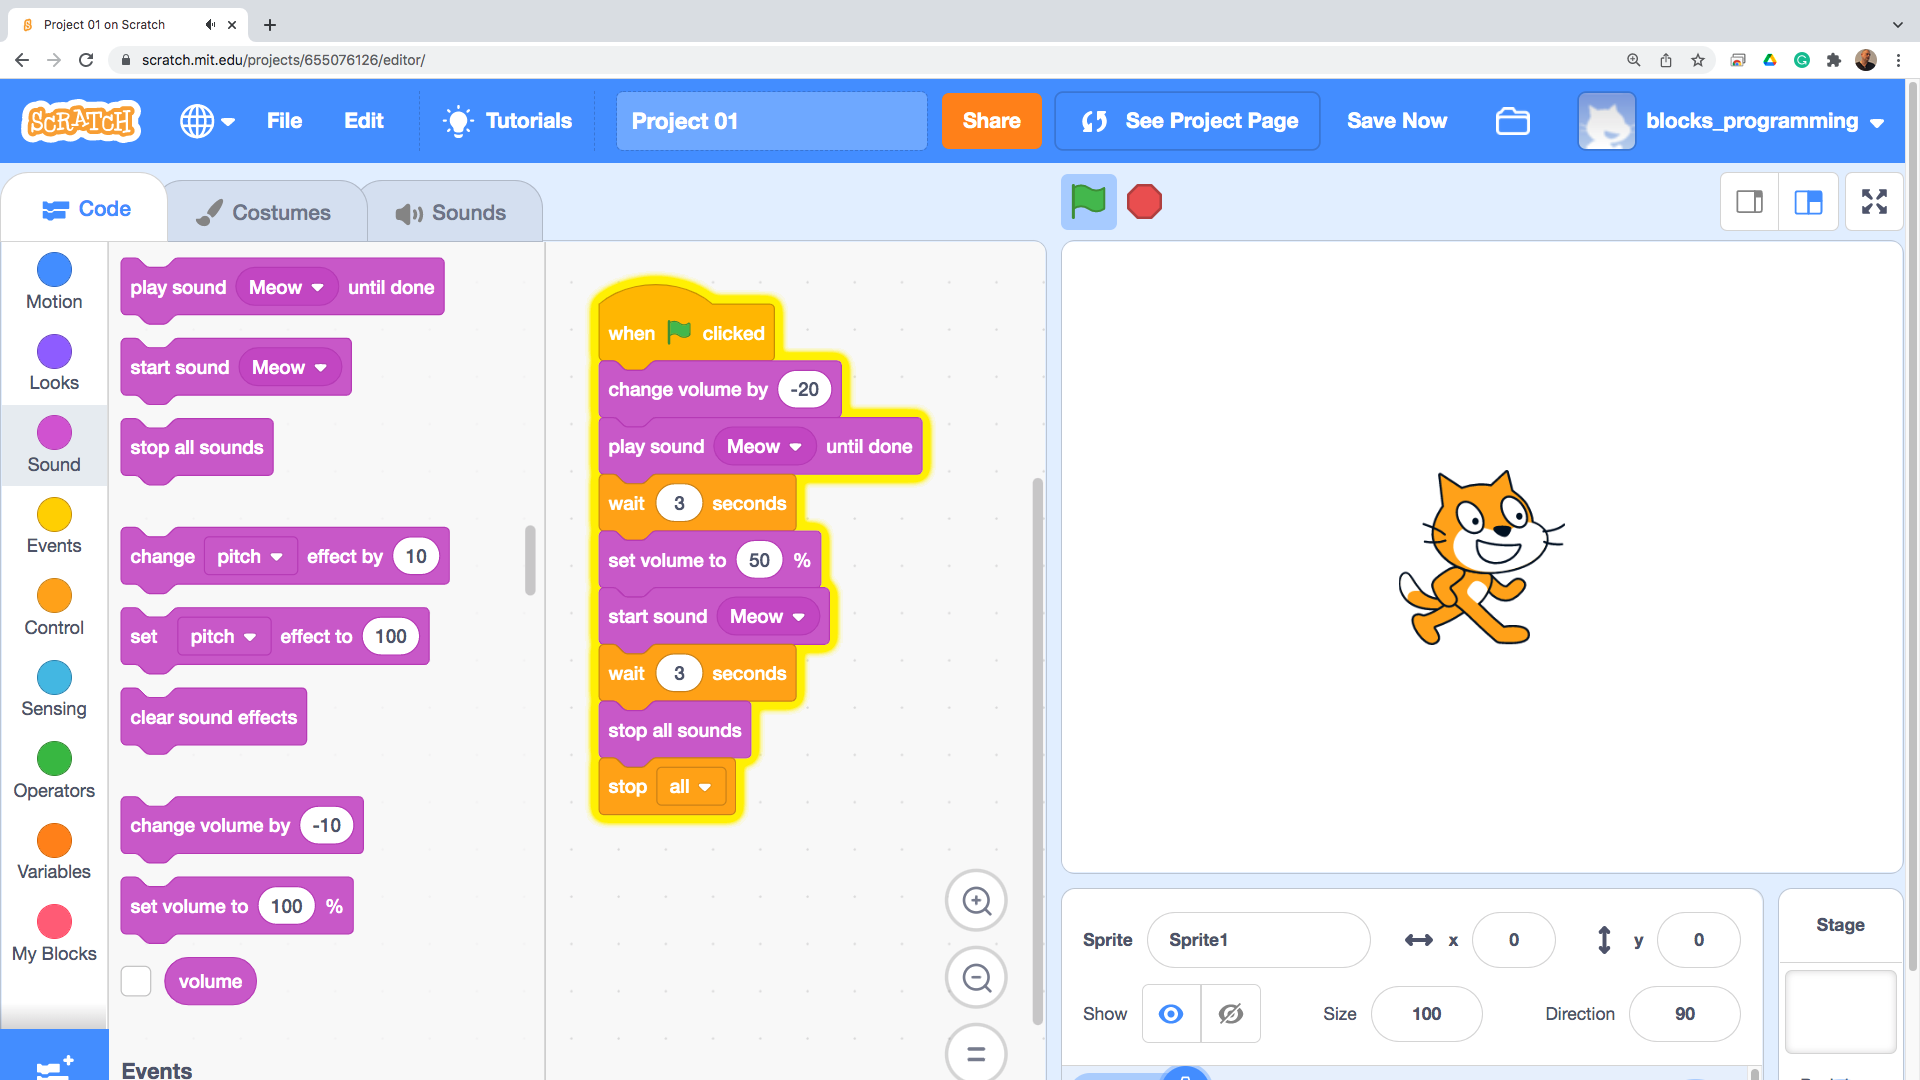
\includegraphics[width=1.0\linewidth,height=0.5\linewidth]{fig020028.png}
   \caption{Volume}
\label{fig020028}
\end{figure}

The orange group of blocks is for events to occur. Events are a tool for executing instructions when there is no explicit cutoff for when program instructions must be performed. Such an event is pressing a button on the keyboard by the user (Fig. \ref{fig020029}).

\begin{figure}[H]
   \centering
   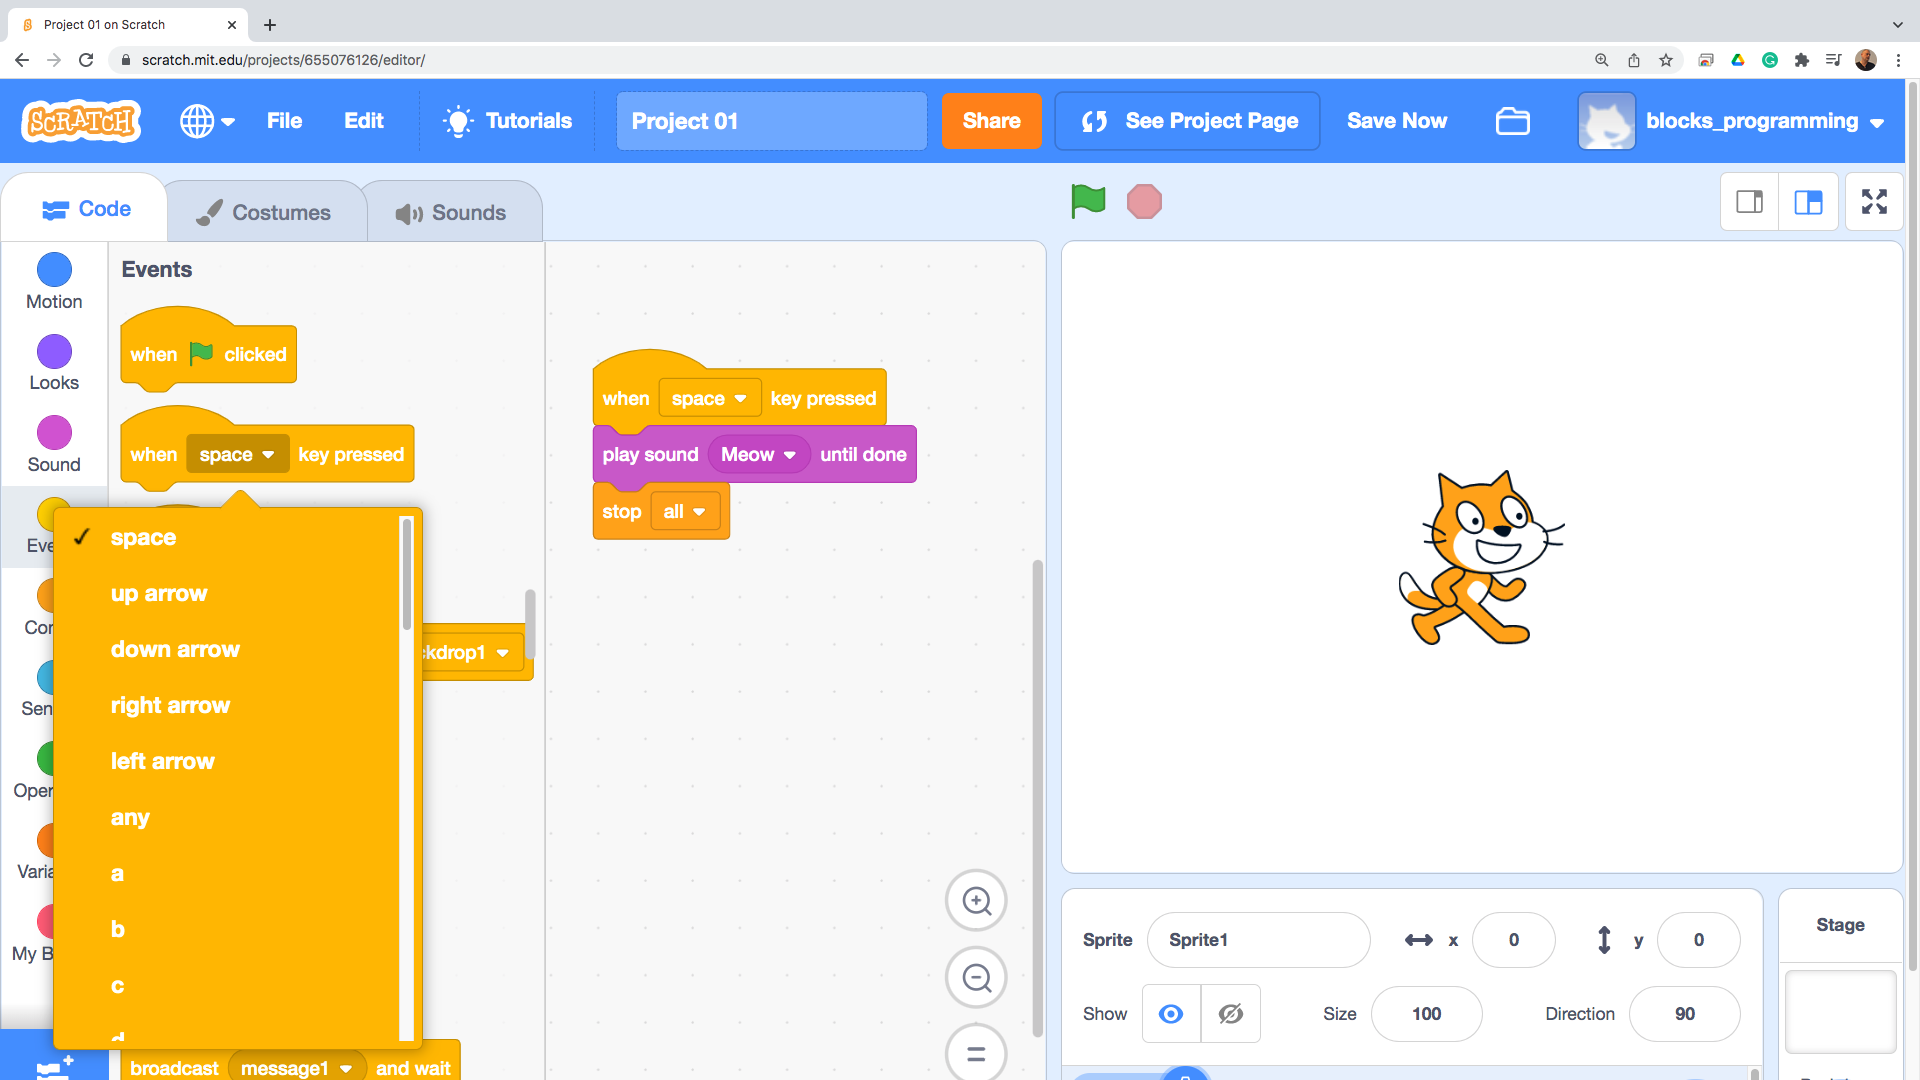
\includegraphics[width=1.0\linewidth,height=0.5\linewidth]{fig020029.png}
   \caption{Key Press Event}
\label{fig020029}
\end{figure}

Mouse clicking on a specific sprite can also be handled using a suitable block (Fig. \ref{fig020030}).

\begin{figure}[H]
   \centering
   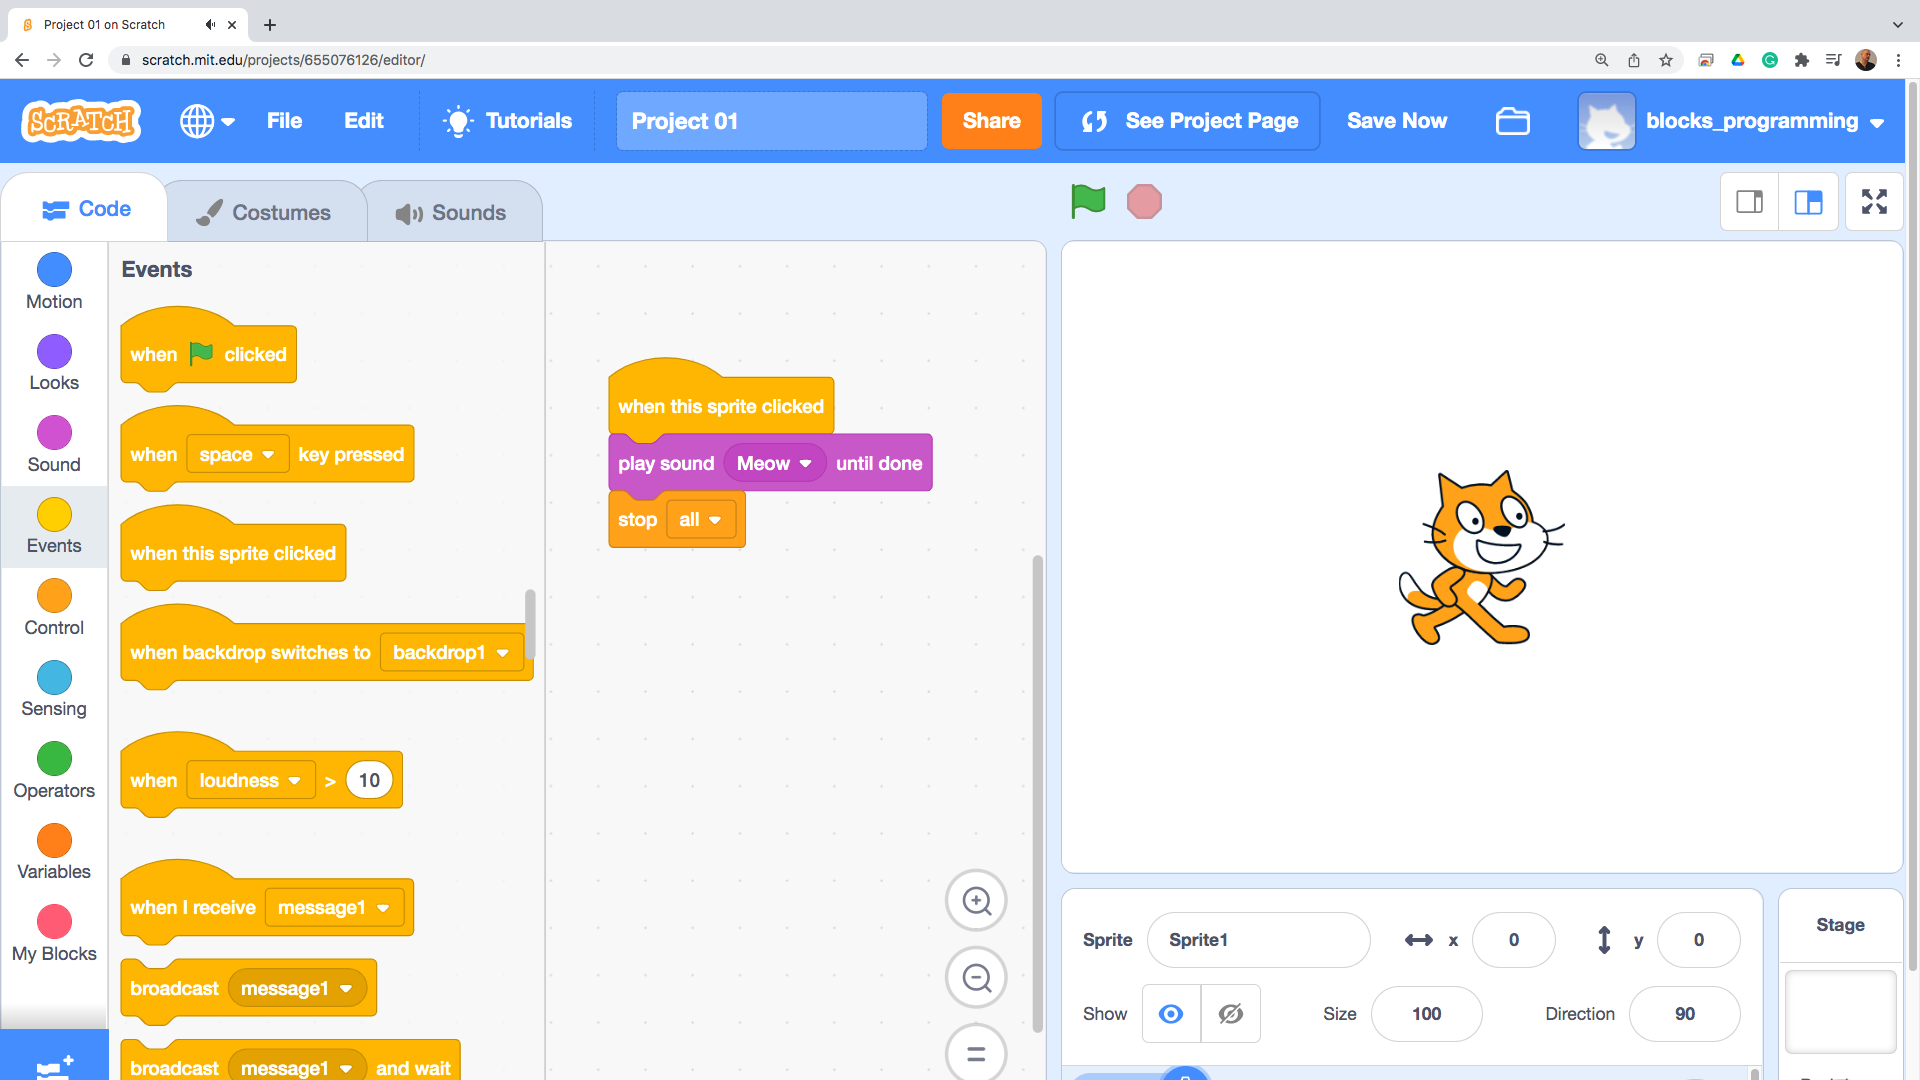
\includegraphics[width=1.0\linewidth,height=0.5\linewidth]{fig020030.png}
   \caption{Mouse Click Event}
\label{fig020030}
\end{figure}

Changing the background can also trigger an event to be handled. A block is provided for this purpose (Fig. \ref{fig020031}).

\begin{figure}[H]
   \centering
   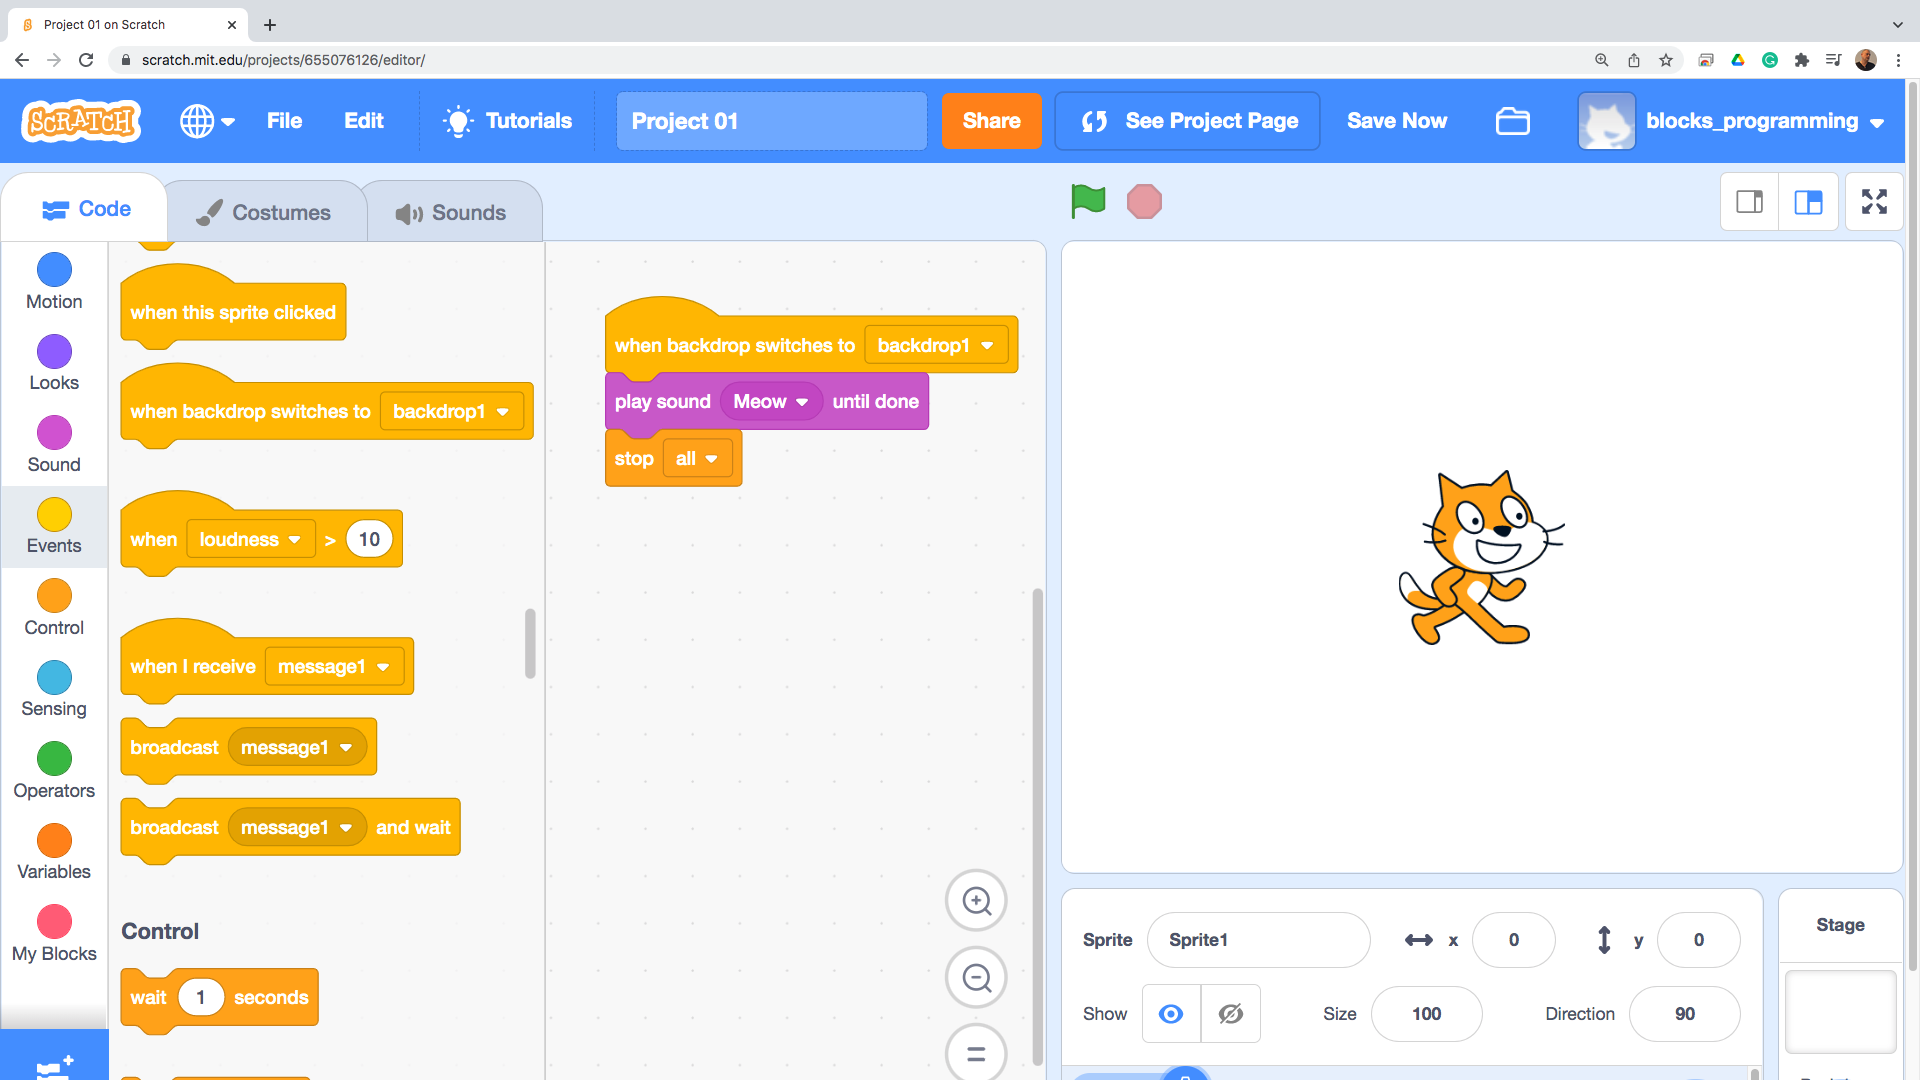
\includegraphics[width=1.0\linewidth,height=0.5\linewidth]{fig020031.png}
   \caption{BackgroundChange Event}
\label{fig020031}
\end{figure}

An event can be caught after a particular time has elapsed to a timer or a certain sound level has been reached (Fig. \ref{fig020032}).

\begin{figure}[H]
   \centering
   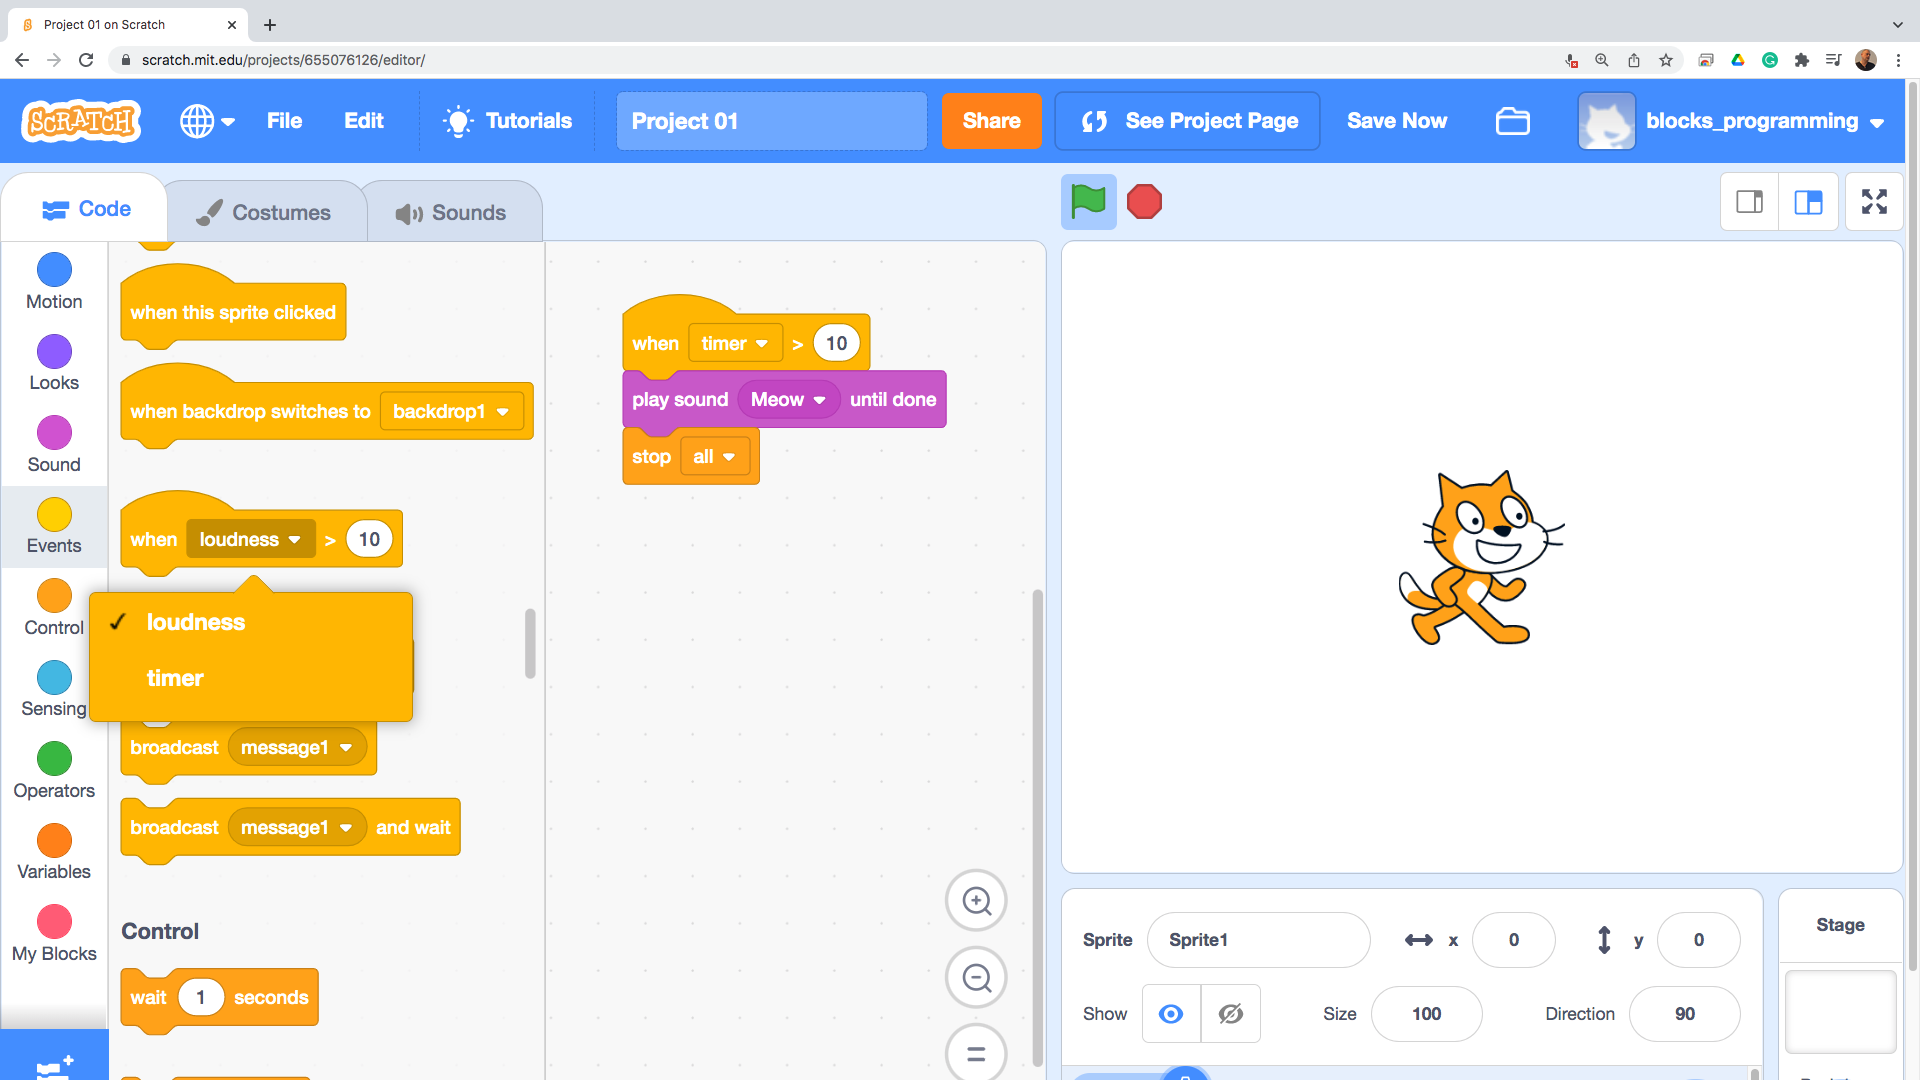
\includegraphics[width=1.0\linewidth,height=0.5\linewidth]{fig020032.png}
   \caption{Timer or sound event}
\label{fig020032}
\end{figure}

Event handling is also associated with a mechanism for sending/receiving messages. One block of instructions can broadcast a predefined message, and another can subscribe to receive precisely that kind of message (Fig. \ref{fig020033}).

\begin{figure}[H]
   \centering
   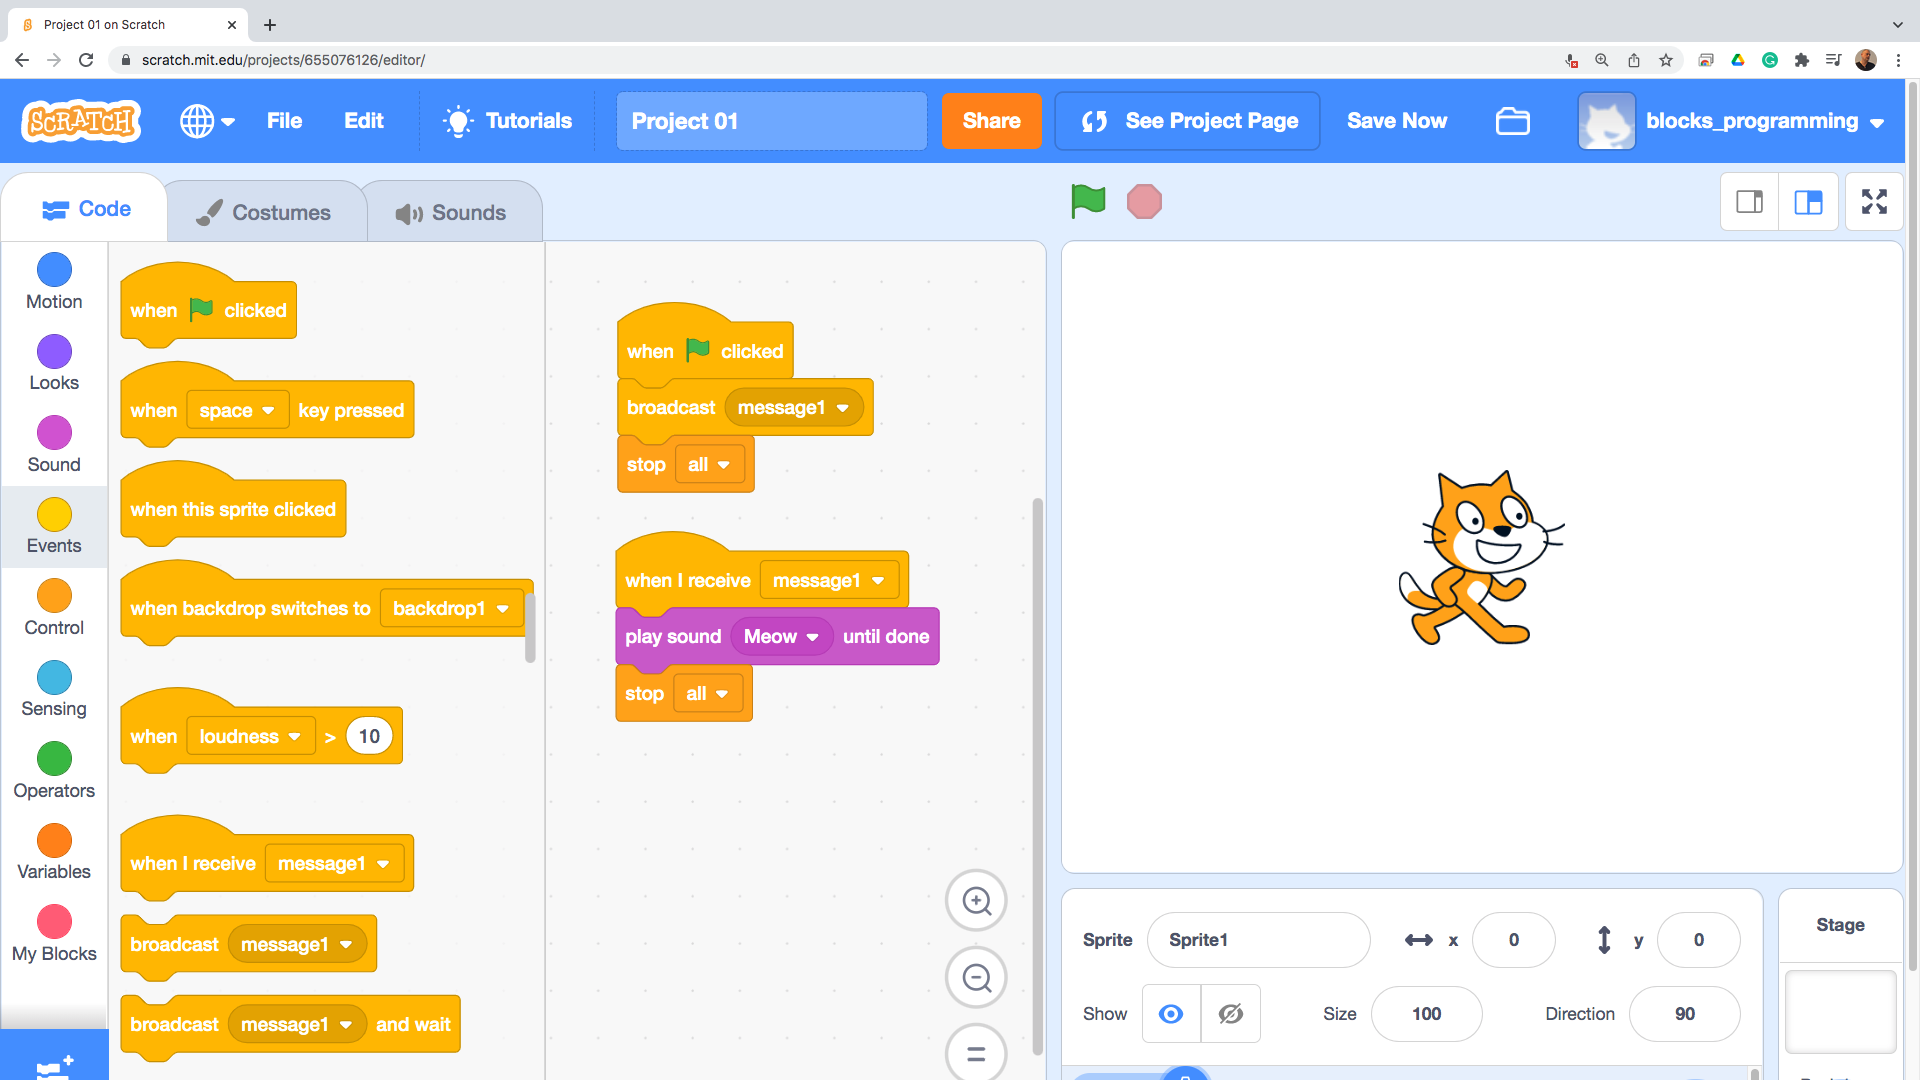
\includegraphics[width=1.0\linewidth,height=0.5\linewidth]{fig020033.png}
   \caption{Broadcasting and receiving messages}
\label{fig020033}
\end{figure}

Since working with the messaging engine may require synchronization, it has a separate block that propagates the message and waits for actions to be taken on its interception (Fig. \ref{fig020034}). The programmer can create different messages to be sent in different situations.

\begin{figure}[H]
   \centering
   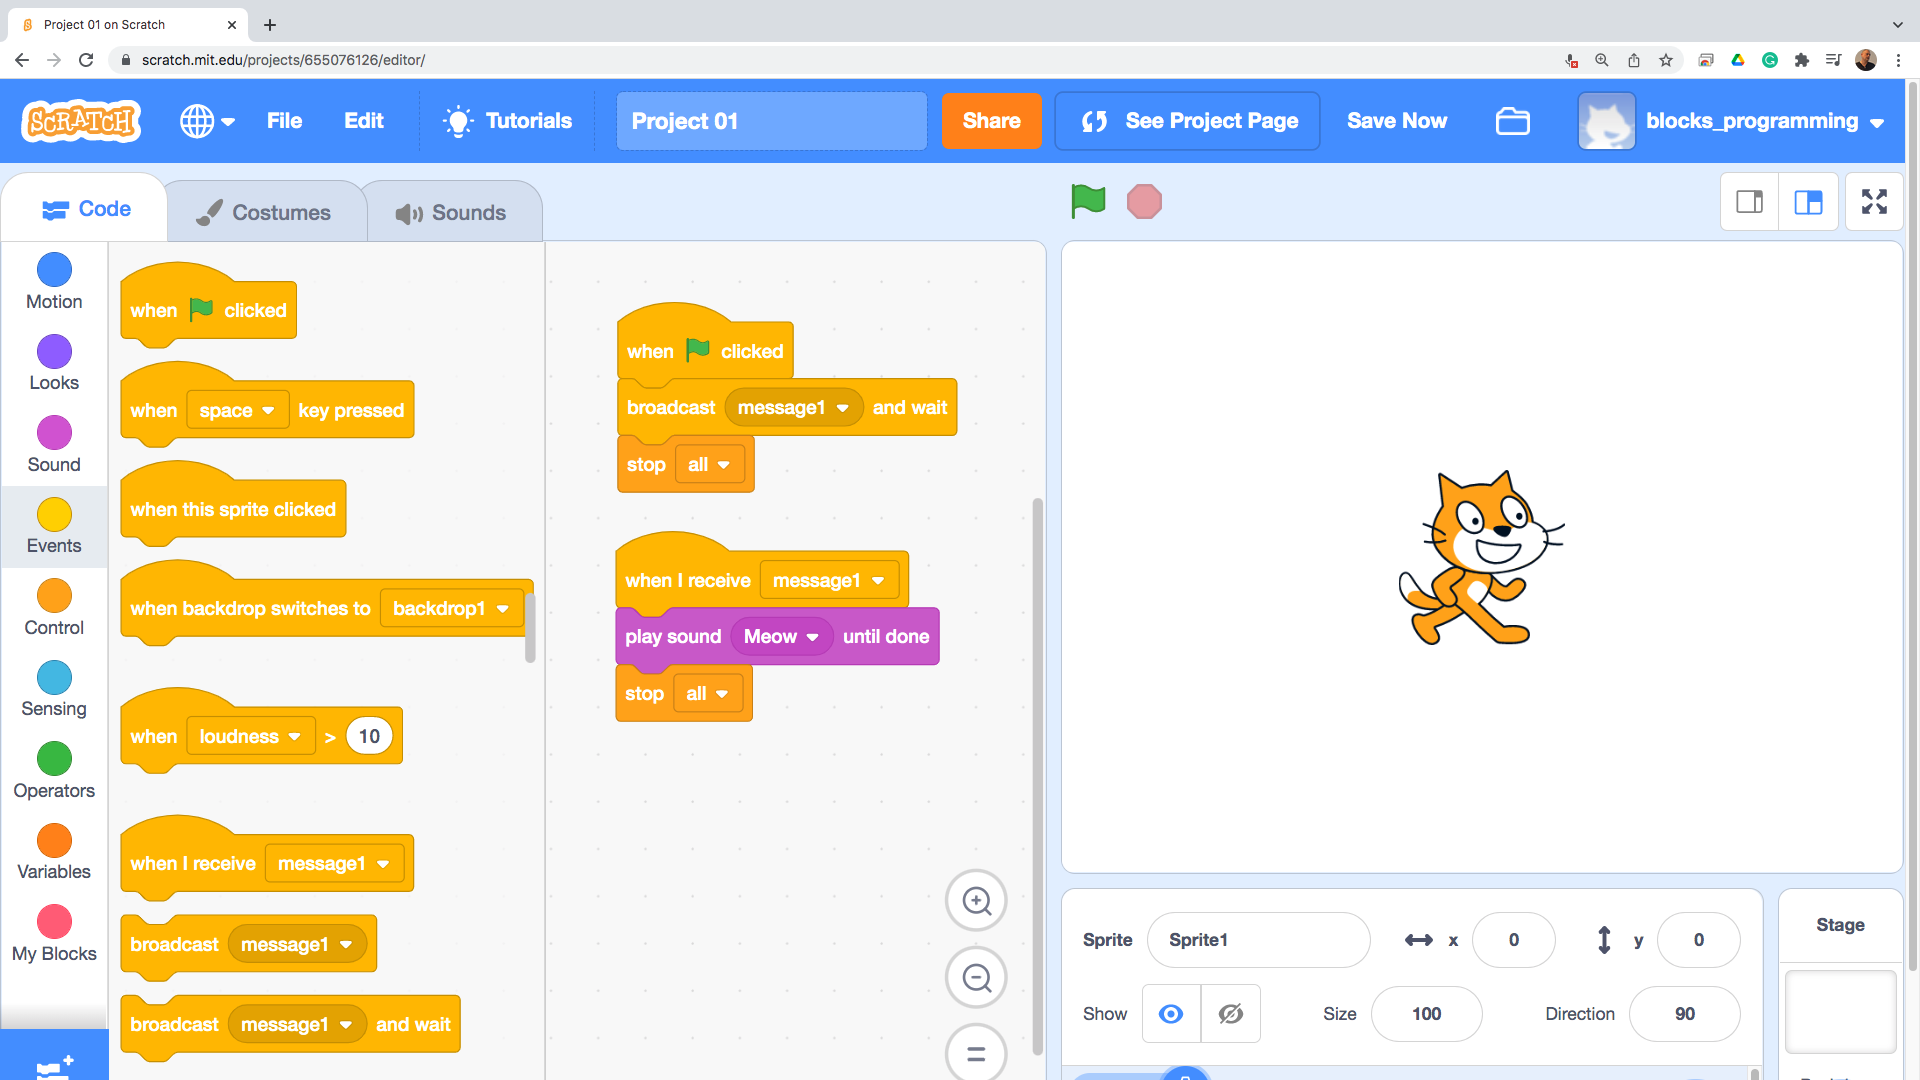
\includegraphics[width=1.0\linewidth,height=0.5\linewidth]{fig020034.png}
   \caption{Propagating a pending message}
\label{fig020034}
\end{figure}

The most essential and valuable blocks are organized in the dark orange group. These blocks define which execution path to take, given the possible choices for executing instructions. When the desire is to perform a specific action repeatedly, with a set number of repetitions, there is a particular block for this purpose (Fig. \ref{fig020035}). Multiple iterations are accomplished in programming using loop constructs, as with this iteration block.

\begin{figure}[H]
   \centering
   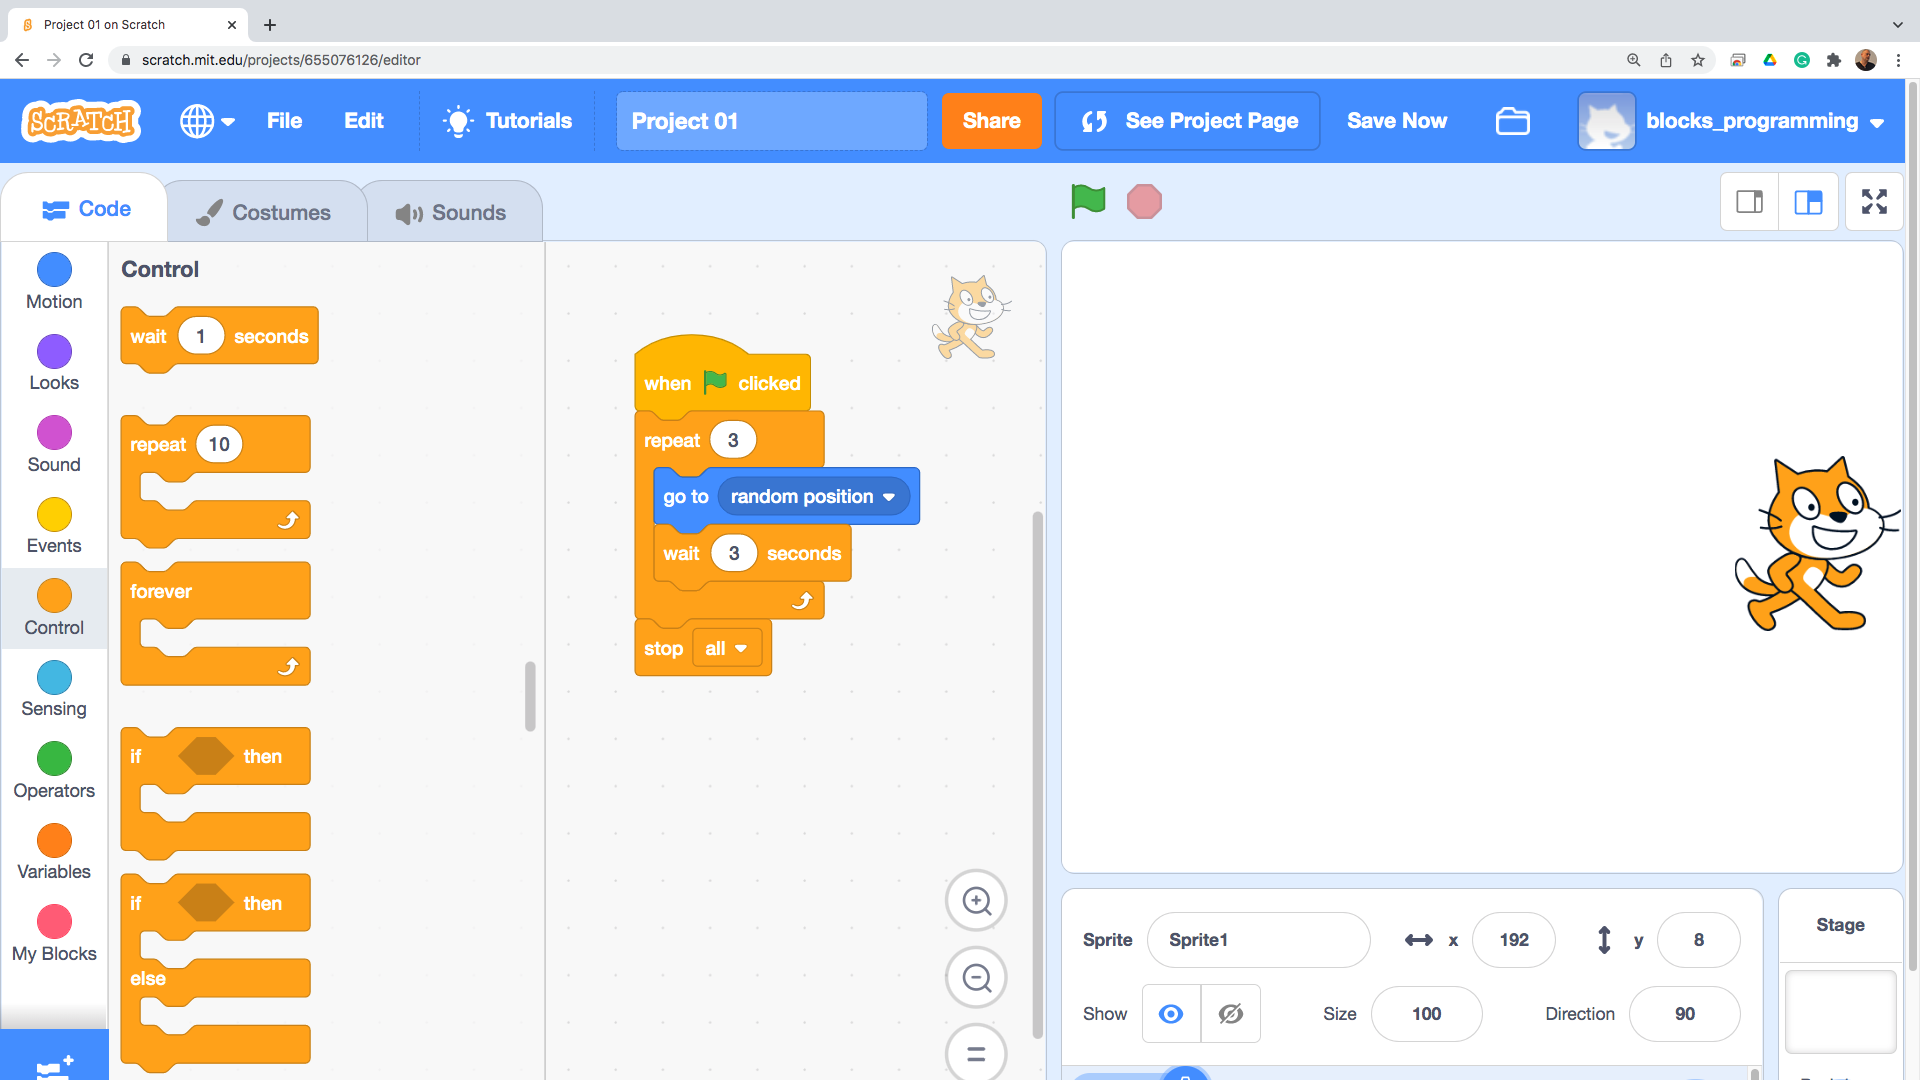
\includegraphics[width=1.0\linewidth,height=0.5\linewidth]{fig020035.png}
   \caption{Fixed number of iterations}
\label{fig020035}
\end{figure}

The word repeat in English means repeat. The number in the pad determines how many repetitions to execute, and the slot in the pad is where the instructions to be repeated are placed. In this example, the kitten is moved to randomly selected coordinates, followed by a predetermined number of seconds to wait. In infrequent situations, there is a need for an infinitely repeating loop, for which a separate block is provided (Fig. \ref{fig020036}).

\begin{figure}[H]
   \centering
   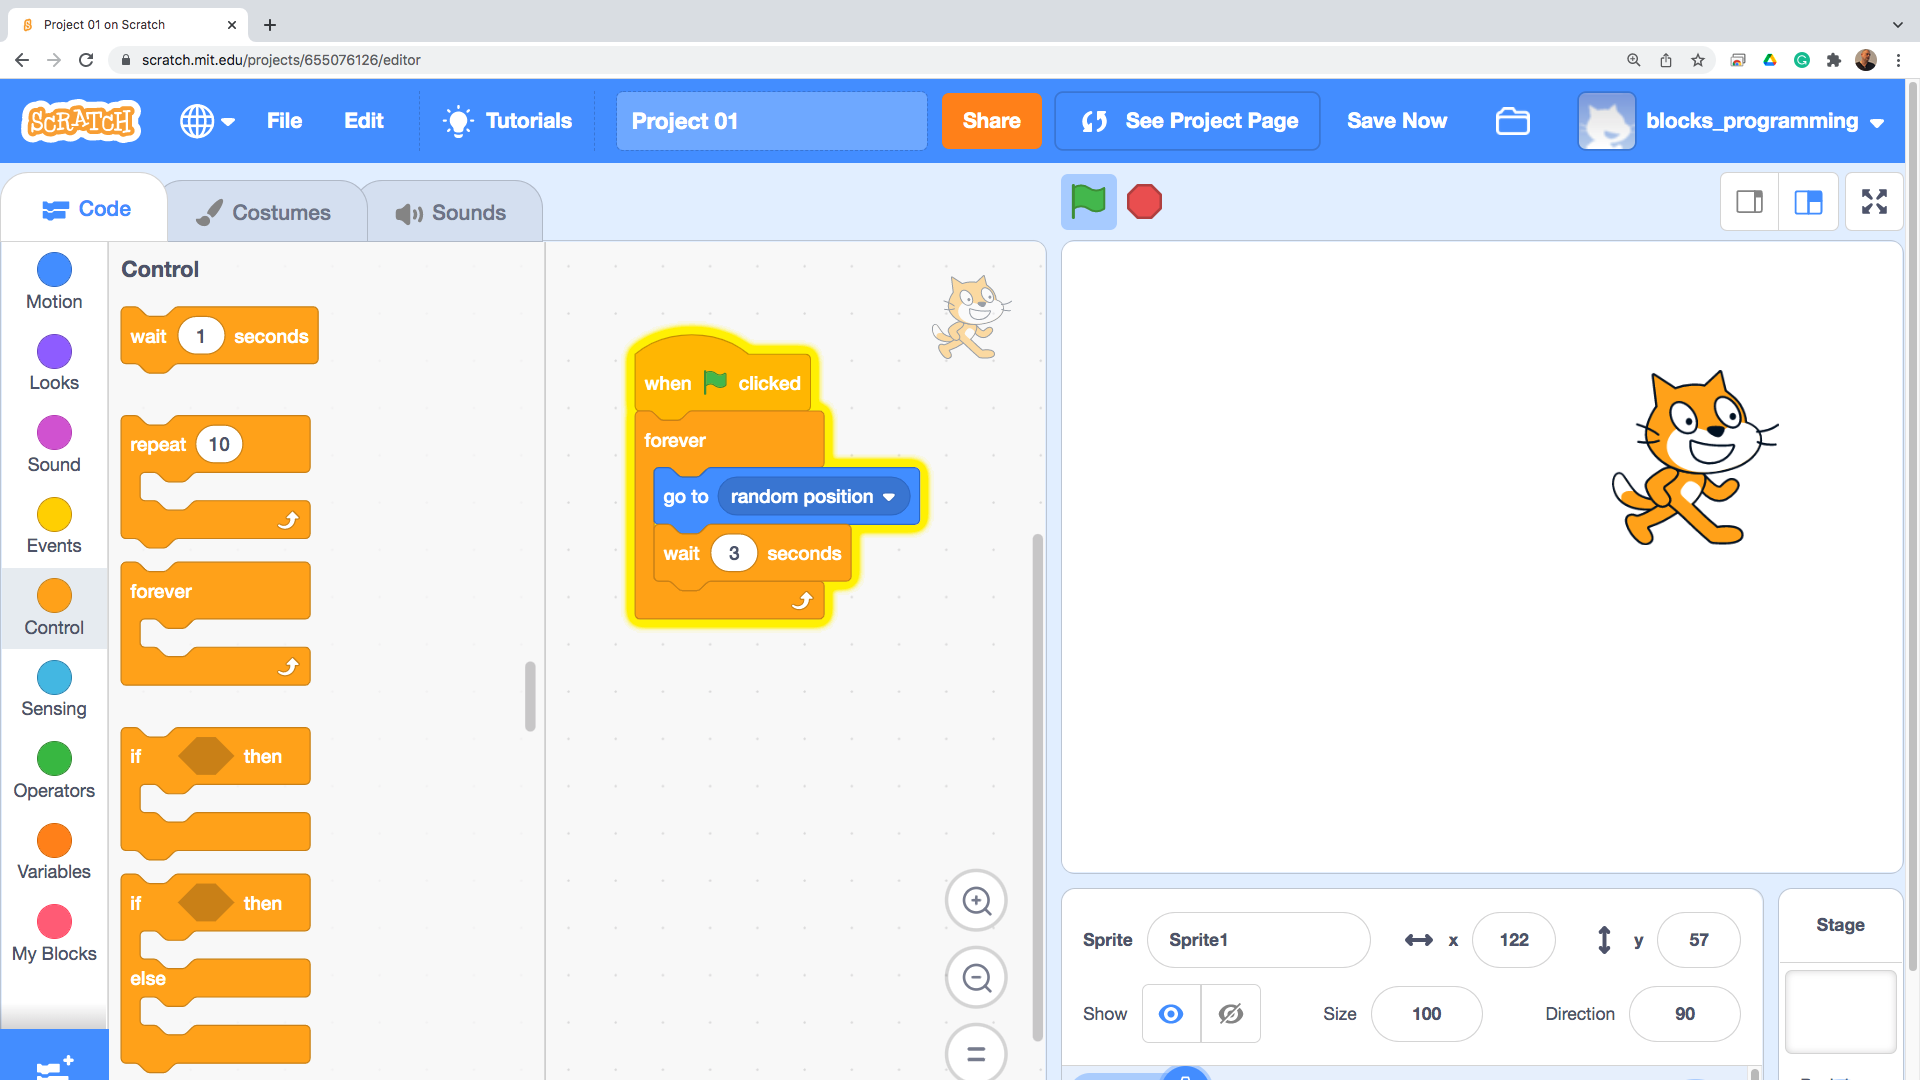
\includegraphics[width=1.0\linewidth,height=0.5\linewidth]{fig020036.png}
   \caption{Infinite Replays}
\label{fig020036}
\end{figure}

The next block is one of the most essential blocks in programming. It is called a conditional execution block (Fig. \ref{fig020037}) or a conditional transition. The block's content is executed only if the condition in its header is fulfilled.

\begin{figure}[H]
   \centering
   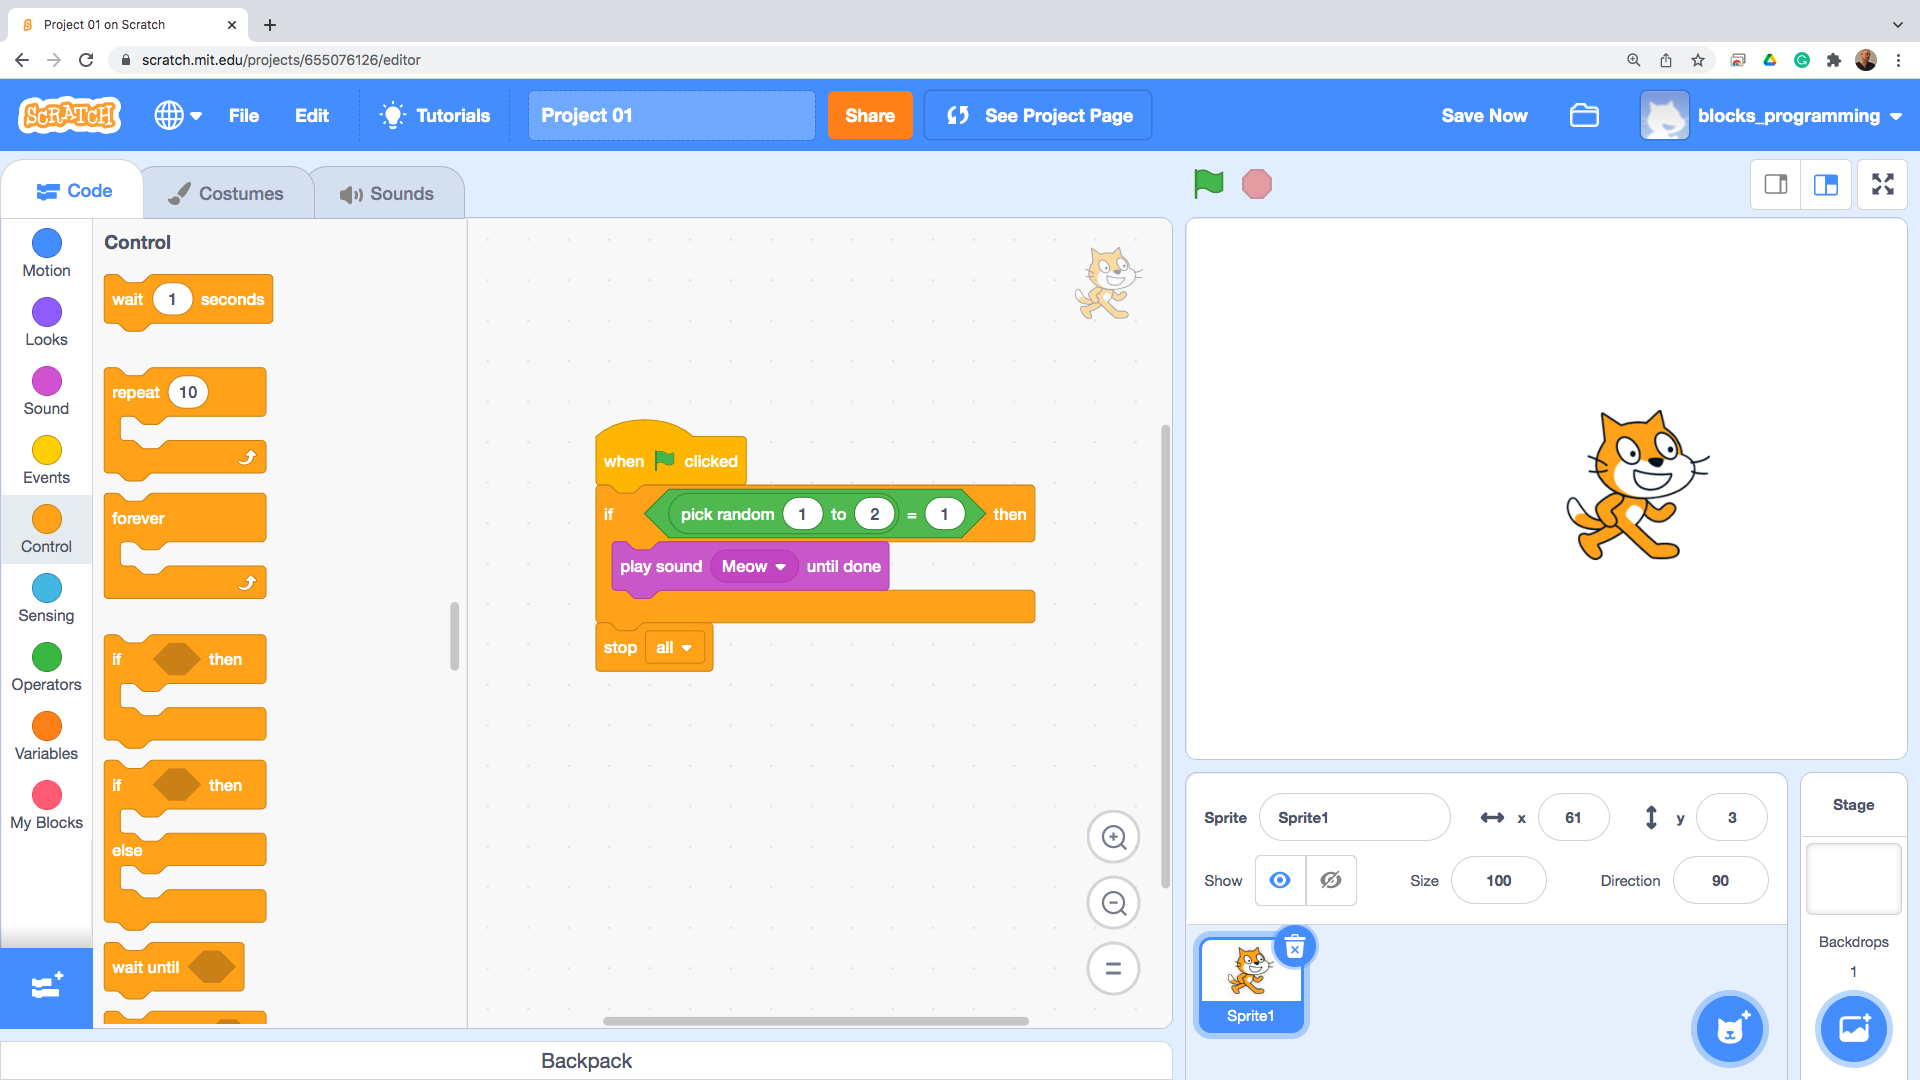
\includegraphics[width=1.0\linewidth,height=0.5\linewidth]{fig020037.png}
   \caption{Execution on condition}
\label{fig020037}
\end{figure}

This dark orange block cannot be used alone. It is always paired with at least one green block and sometimes with two, as in the current example. Some of the green blocks are irregular hexagons made to fit into the header of some dark orange blocks. The hexagonal block has an oval slot into which some green oval blocks fit. In the example, a green block is selected, which requires equality to a specific number, and a random number generator is used for the oval block according to a predetermined interval. If the condition in the header of the conditional transition block is not met, then the body is skipped, and the following instructions are after the block is passed. The block for conditional transition also has a variant in which slots are provided for the execution of both possibilities – a true or a false condition (Fig. \ref{fig020038}). If the condition is met, the first instruction block is executed. The second block of instructions is executed if the condition is not met.

\begin{figure}[H]
   \centering
   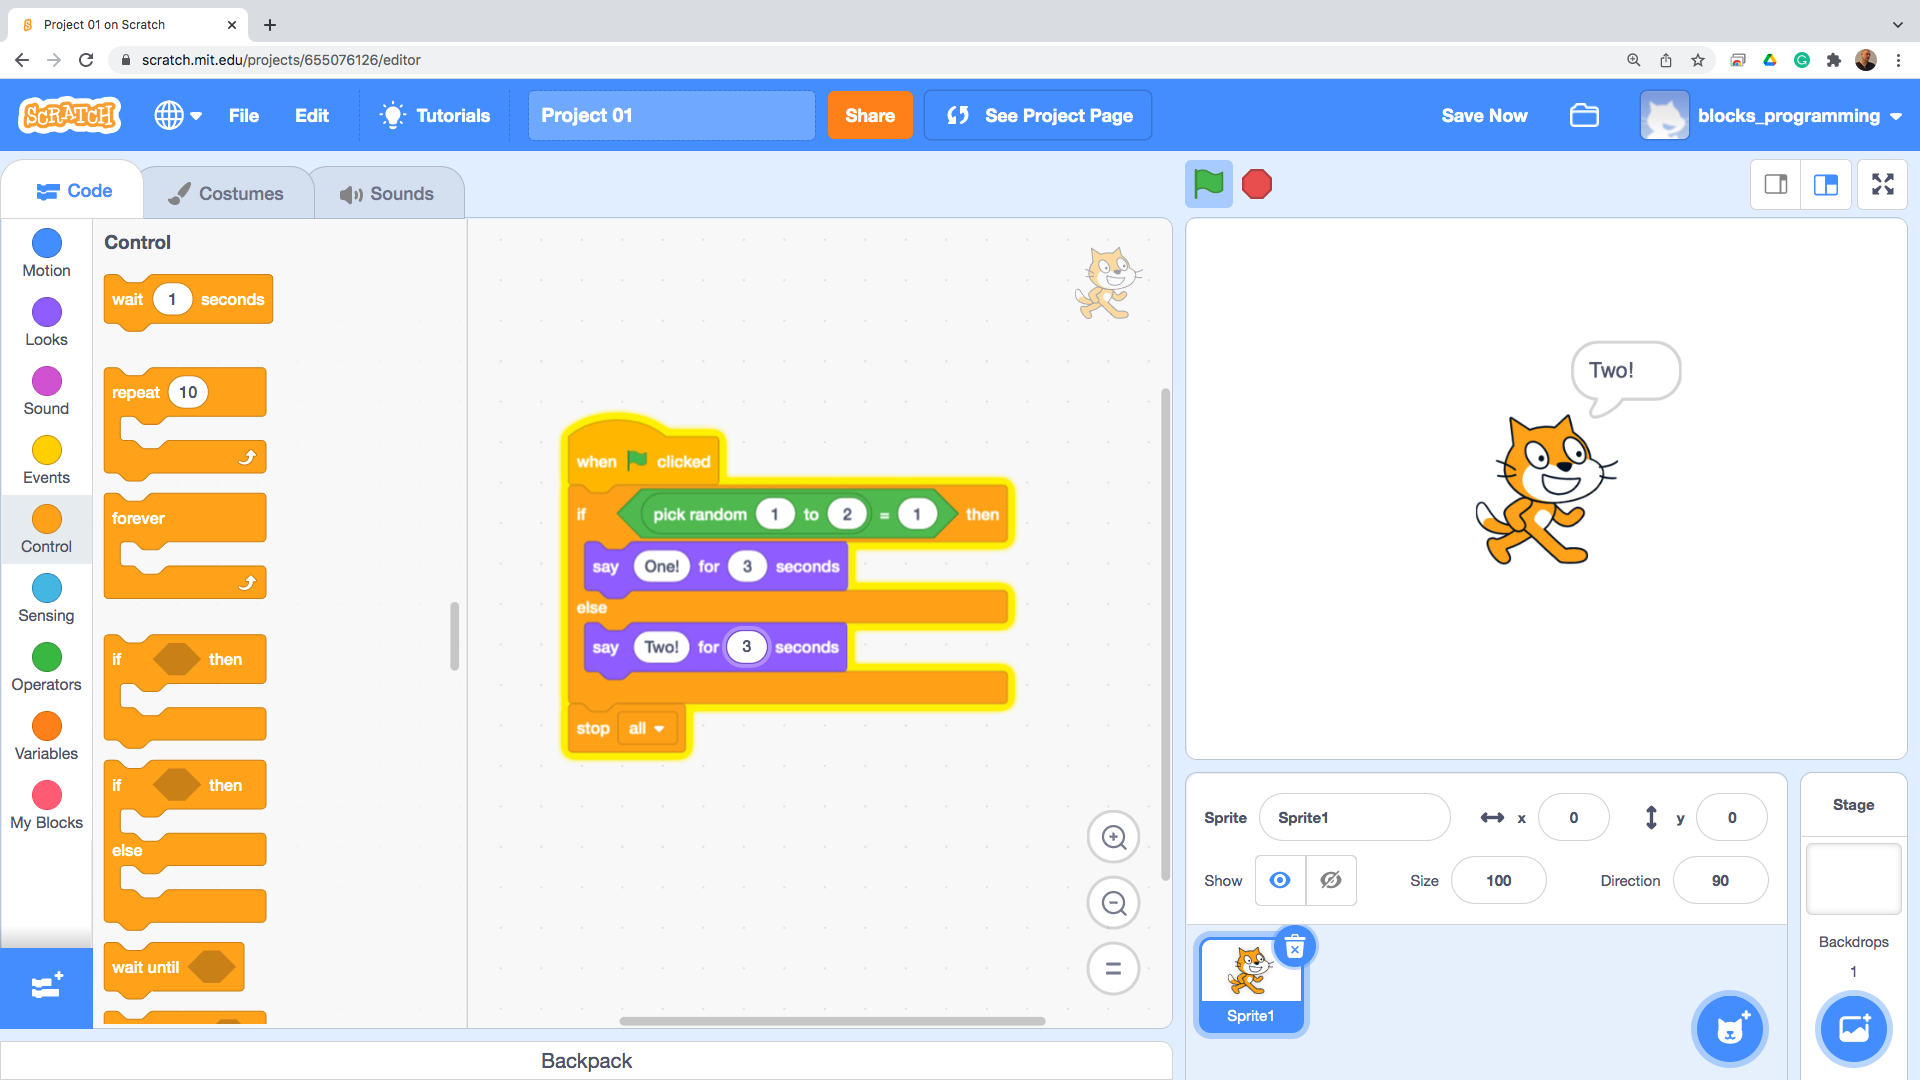
\includegraphics[width=1.0\linewidth,height=0.5\linewidth]{fig020038.png}
   \caption{Execution on condition with alternative}
\label{fig020038}
\end{figure}

The next exciting block is waiting until a particular event happens. In this case, the event is the sprite being touched with the mouse (Fig. \ref{fig020039}). If this touch happens, the execution of the program continues to the next block. What event is expected is defined by an additional block (light blue) with the shape of an irregular hexagon.

\begin{figure}[H]
   \centering
   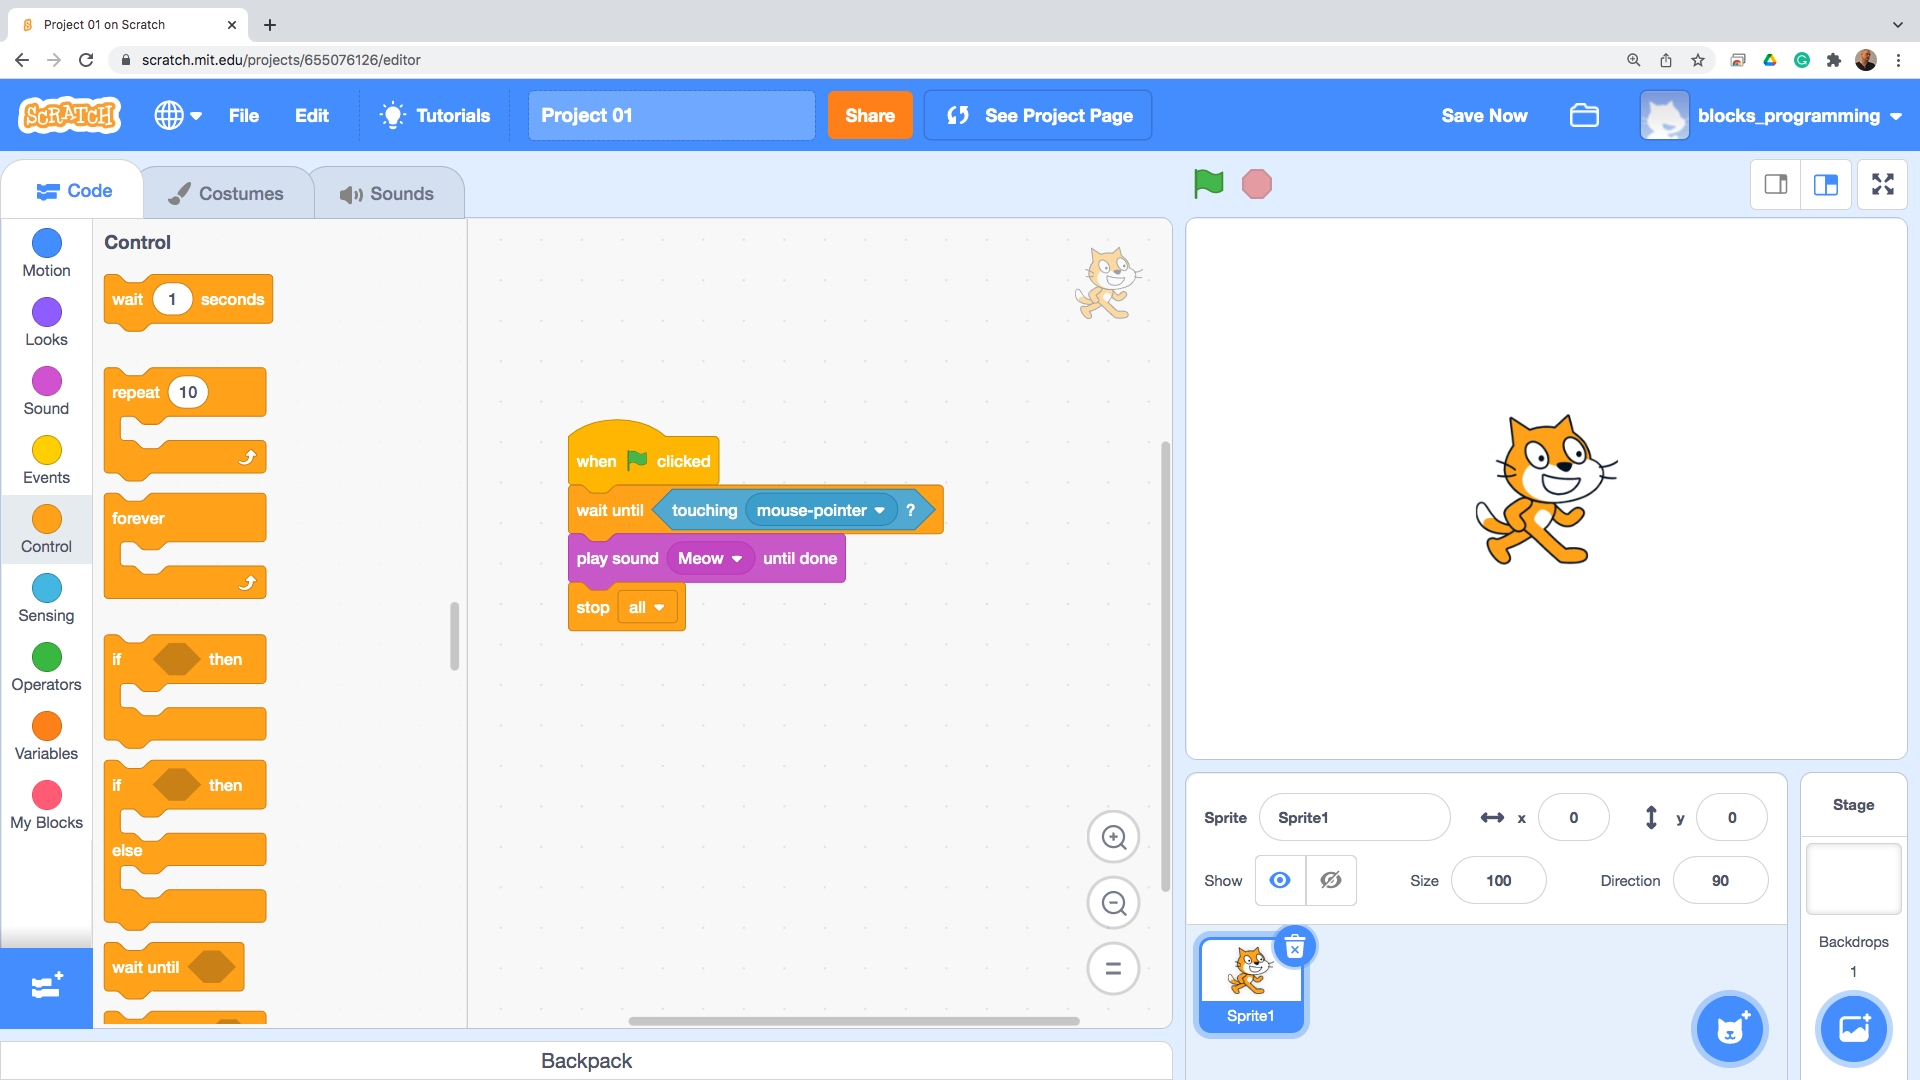
\includegraphics[width=1.0\linewidth,height=0.5\linewidth]{fig020039.png}
   \caption{Waiting condition}
\label{fig020039}
\end{figure}

The last three blocks in the dark orange group must be demonstrated together (Fig. \ref{fig020040}). The first block sets a new chain of instructions when a particular sprite is cloned (a copy of the original sprite). The second block serves to clone the current sprite. And the third block serves to delete the current sprite.

\begin{figure}[H]
   \centering
   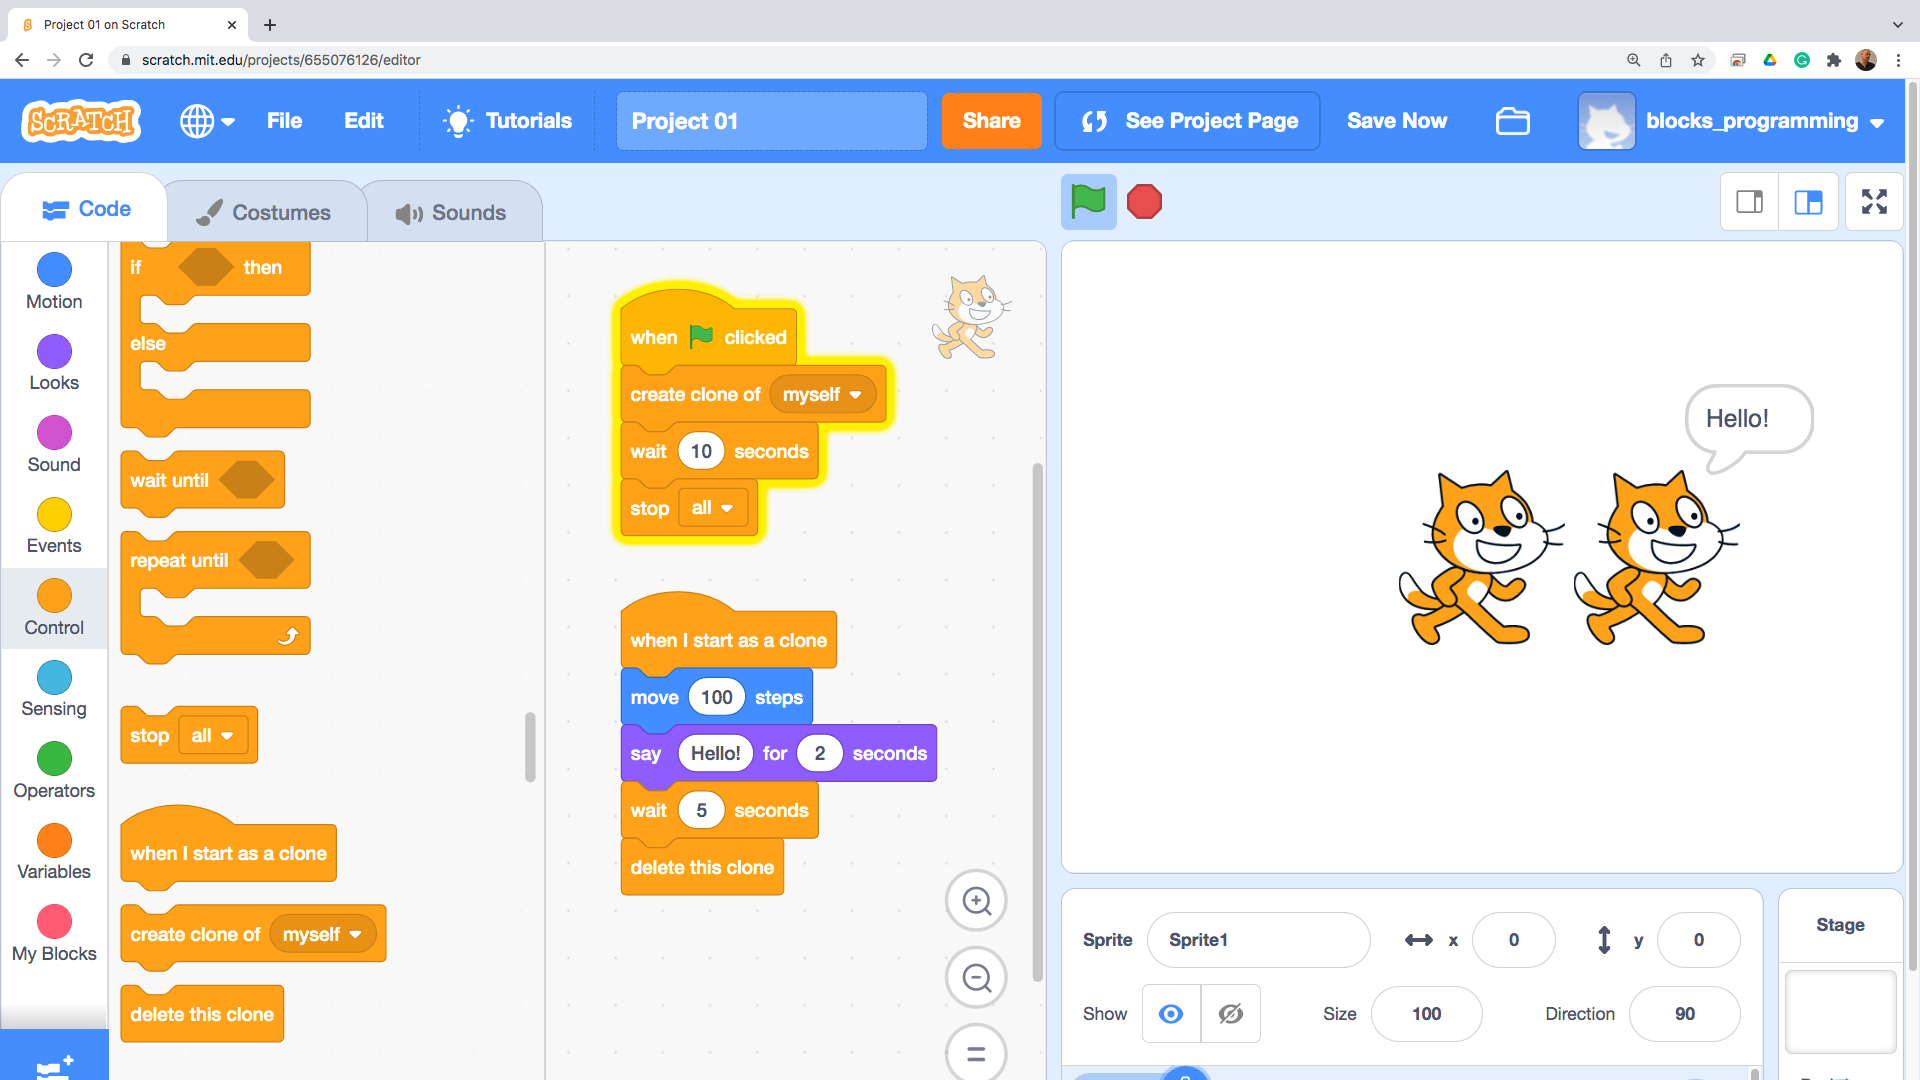
\includegraphics[width=1.0\linewidth,height=0.5\linewidth]{fig020040.png}
   \caption{Clone Sprites}
\label{fig020040}
\end{figure}

The group of light blue blocks is dedicated to interactions related to the sprite. The second block in the group is intended to fulfill a condition when the sprite touches a particular color. The block has a hexagonal shape, suggesting it is designed for embedding. To demonstrate the operation of this block, a loop will be run that will move the kitten to random coordinates and wait a small time interval before the next move (Fig. \ref{fig020041}).

\begin{figure}[H]
   \centering
   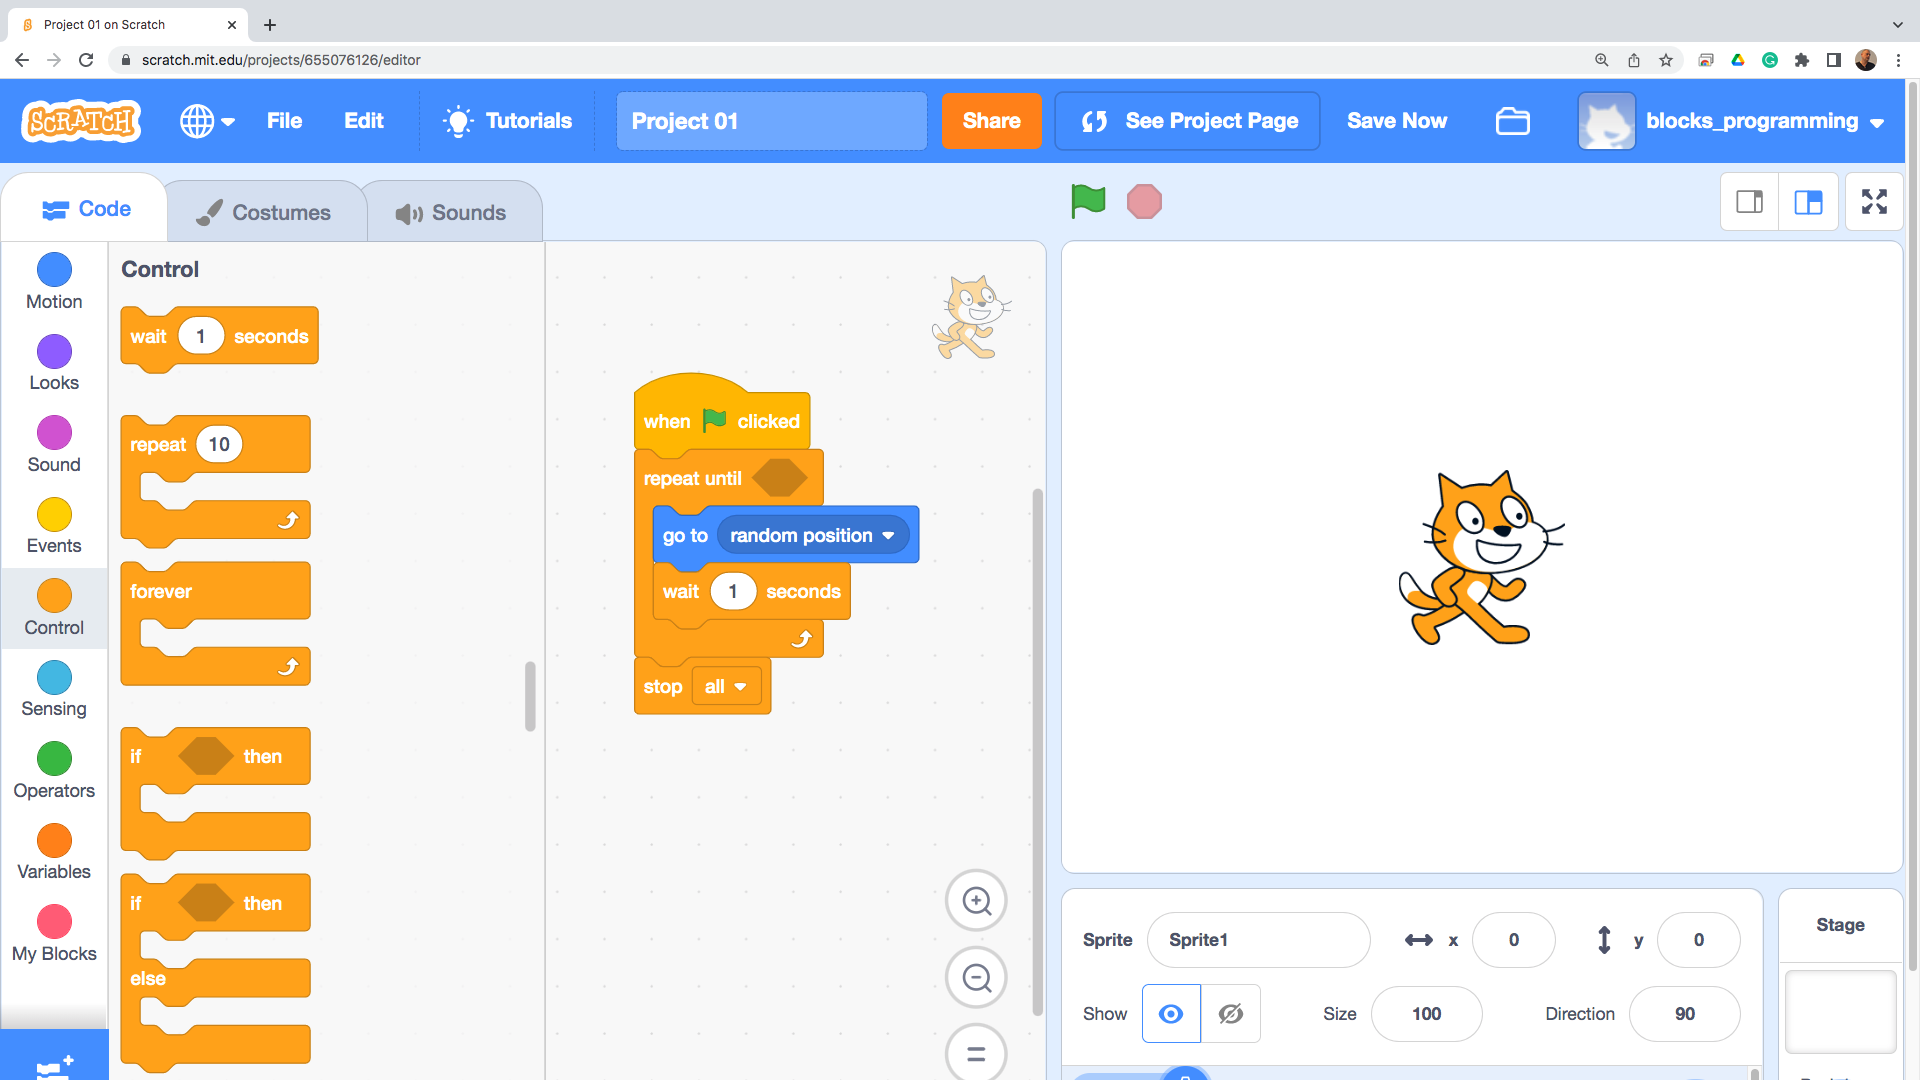
\includegraphics[width=1.0\linewidth,height=0.5\linewidth]{fig020041.png}
   \caption{Cyclical jump of random coordinates}
\label{fig020041}
\end{figure}

A loop made like this will loop endlessly since no end condition is set. In the end condition, I want to place the block defining the touch of color. We will add a new sprite to the scene (Fig. \ref{fig020042}) of a red apple (Fig. \ref{fig020043}), which the kitten must catch. Once he catches her, he will stop prompting and meow (Fig. \ref{fig020044}).

\begin{figure}[H]
   \centering
   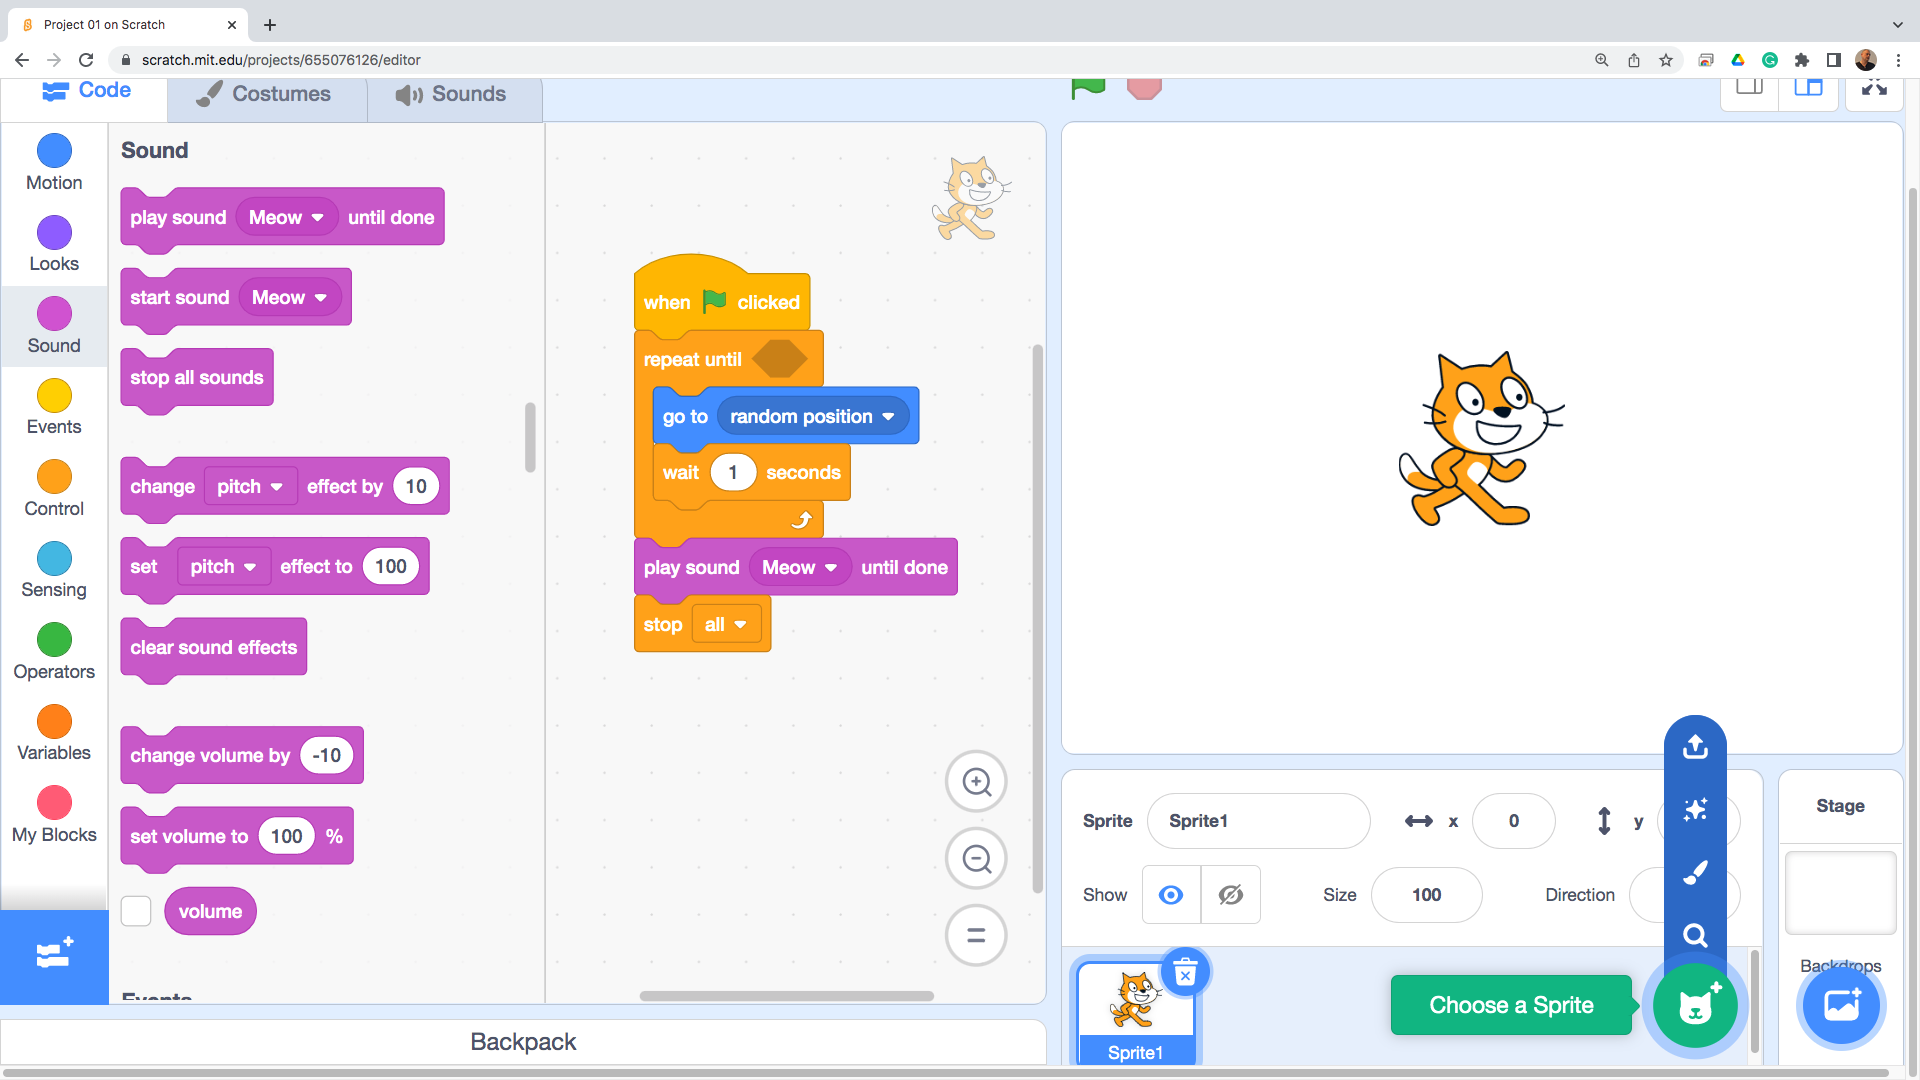
\includegraphics[width=1.0\linewidth,height=0.5\linewidth]{fig020042.png}
   \caption{Add sprite}
\label{fig020042}
\end{figure}

\begin{figure}[H]
   \centering
   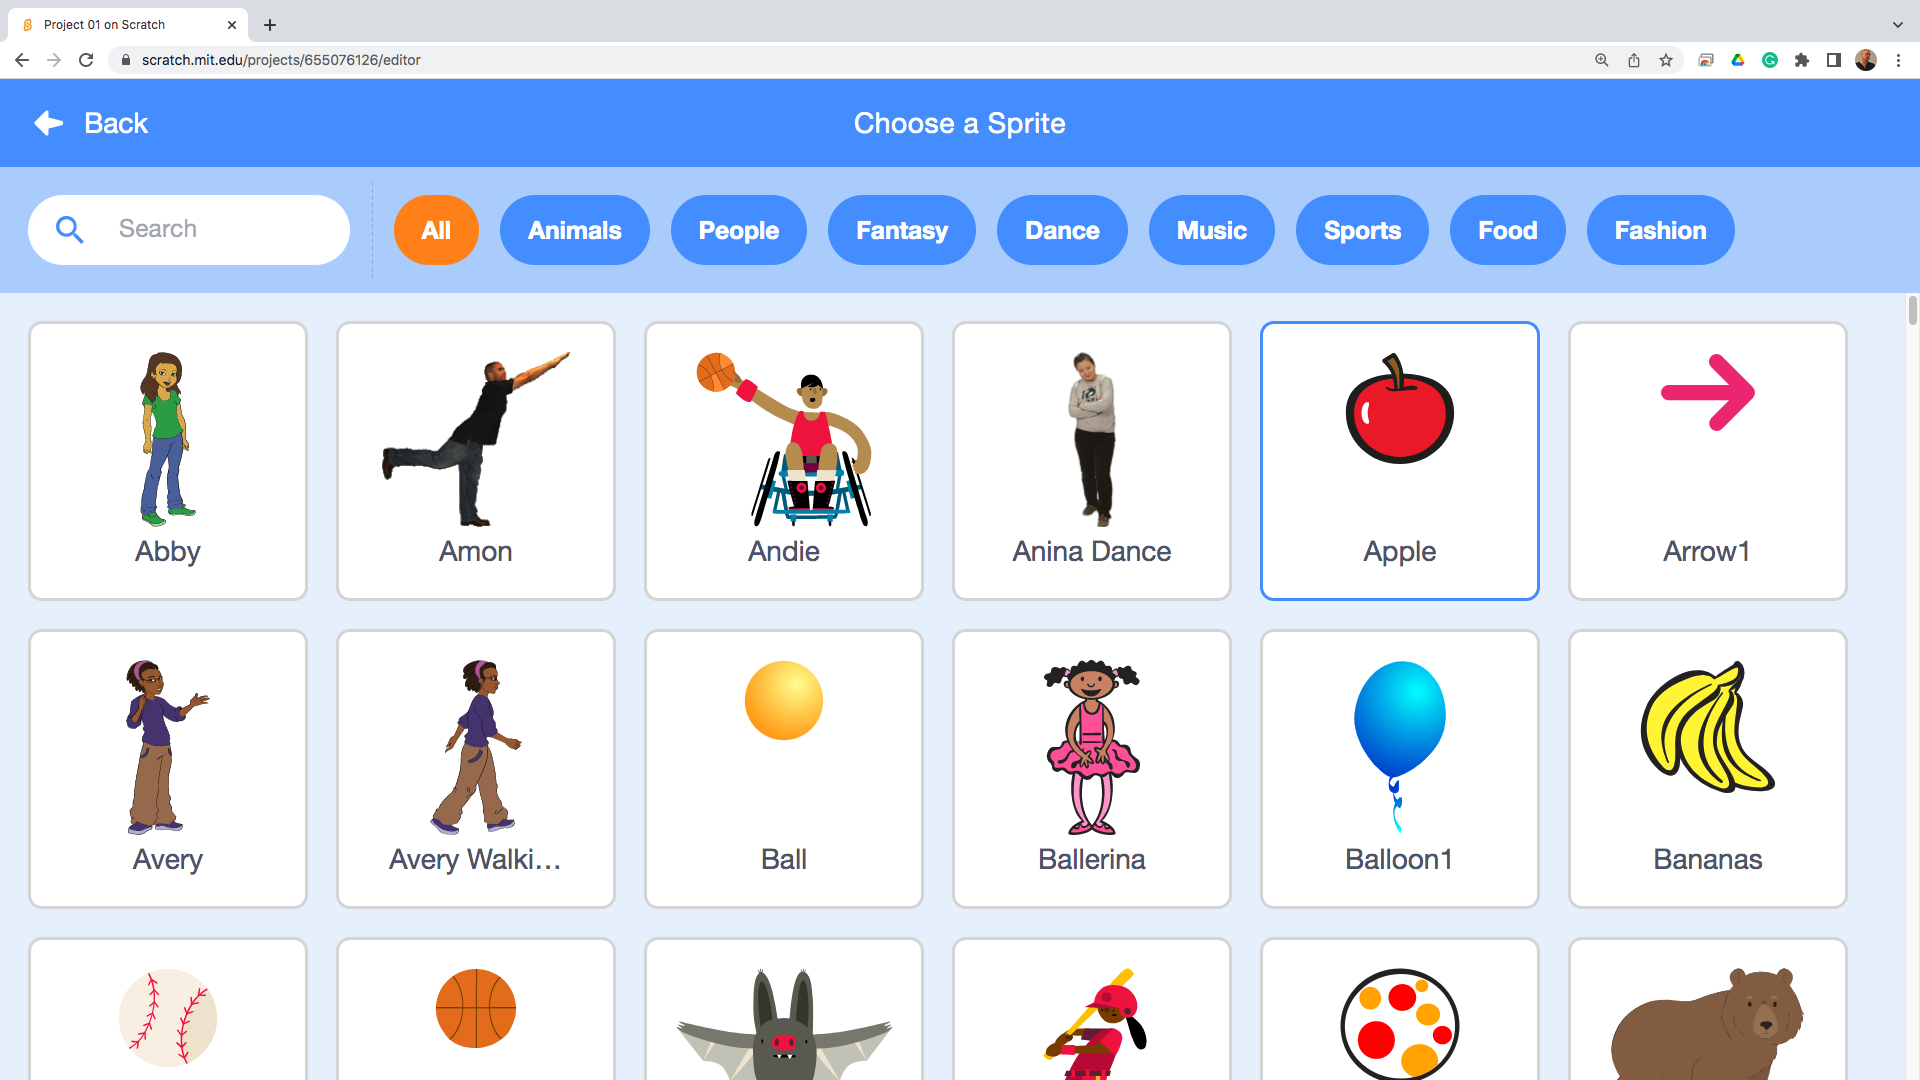
\includegraphics[width=1.0\linewidth,height=0.5\linewidth]{fig020043.png}
   \caption{Choose sprite from gallery}
\label{fig020043}
\end{figure}

\begin{figure}[H]
   \centering
   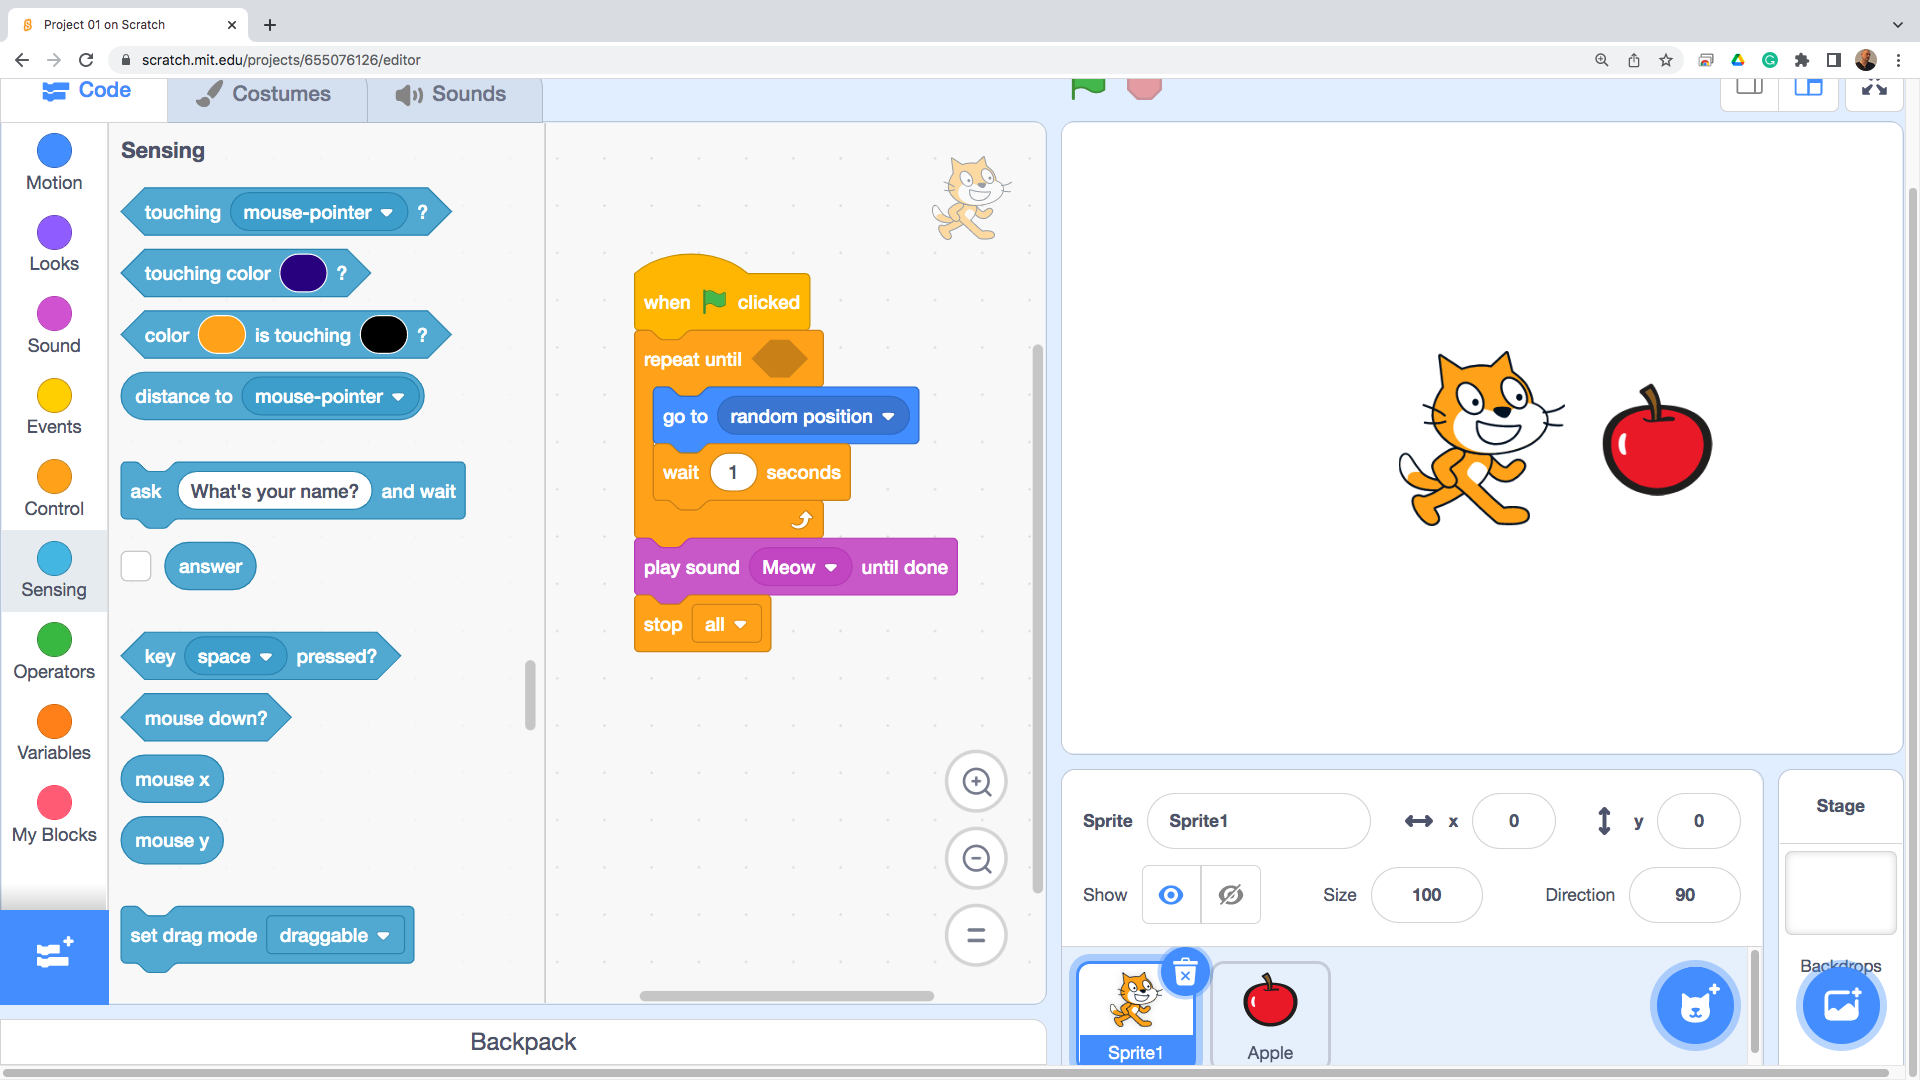
\includegraphics[width=1.0\linewidth,height=0.5\linewidth]{fig020044.png}
   \caption{Positioning the apple}
\label{fig020044}
\end{figure}

One of the most common problems when working with sprites is whether two sprites touch or overlap. There are various techniques for detecting collisions between sprites, but one of the most effective is touching a particular color. Modern computers work with just over 16 million different colors. A judicious selection of the characters' colors can give limitless possibilities for detecting collisions. Since the apple is red, the choice to end the cycle is when the kitten touches the red color (Fig. \ref{fig020045}).

\begin{figure}[H]
   \centering
   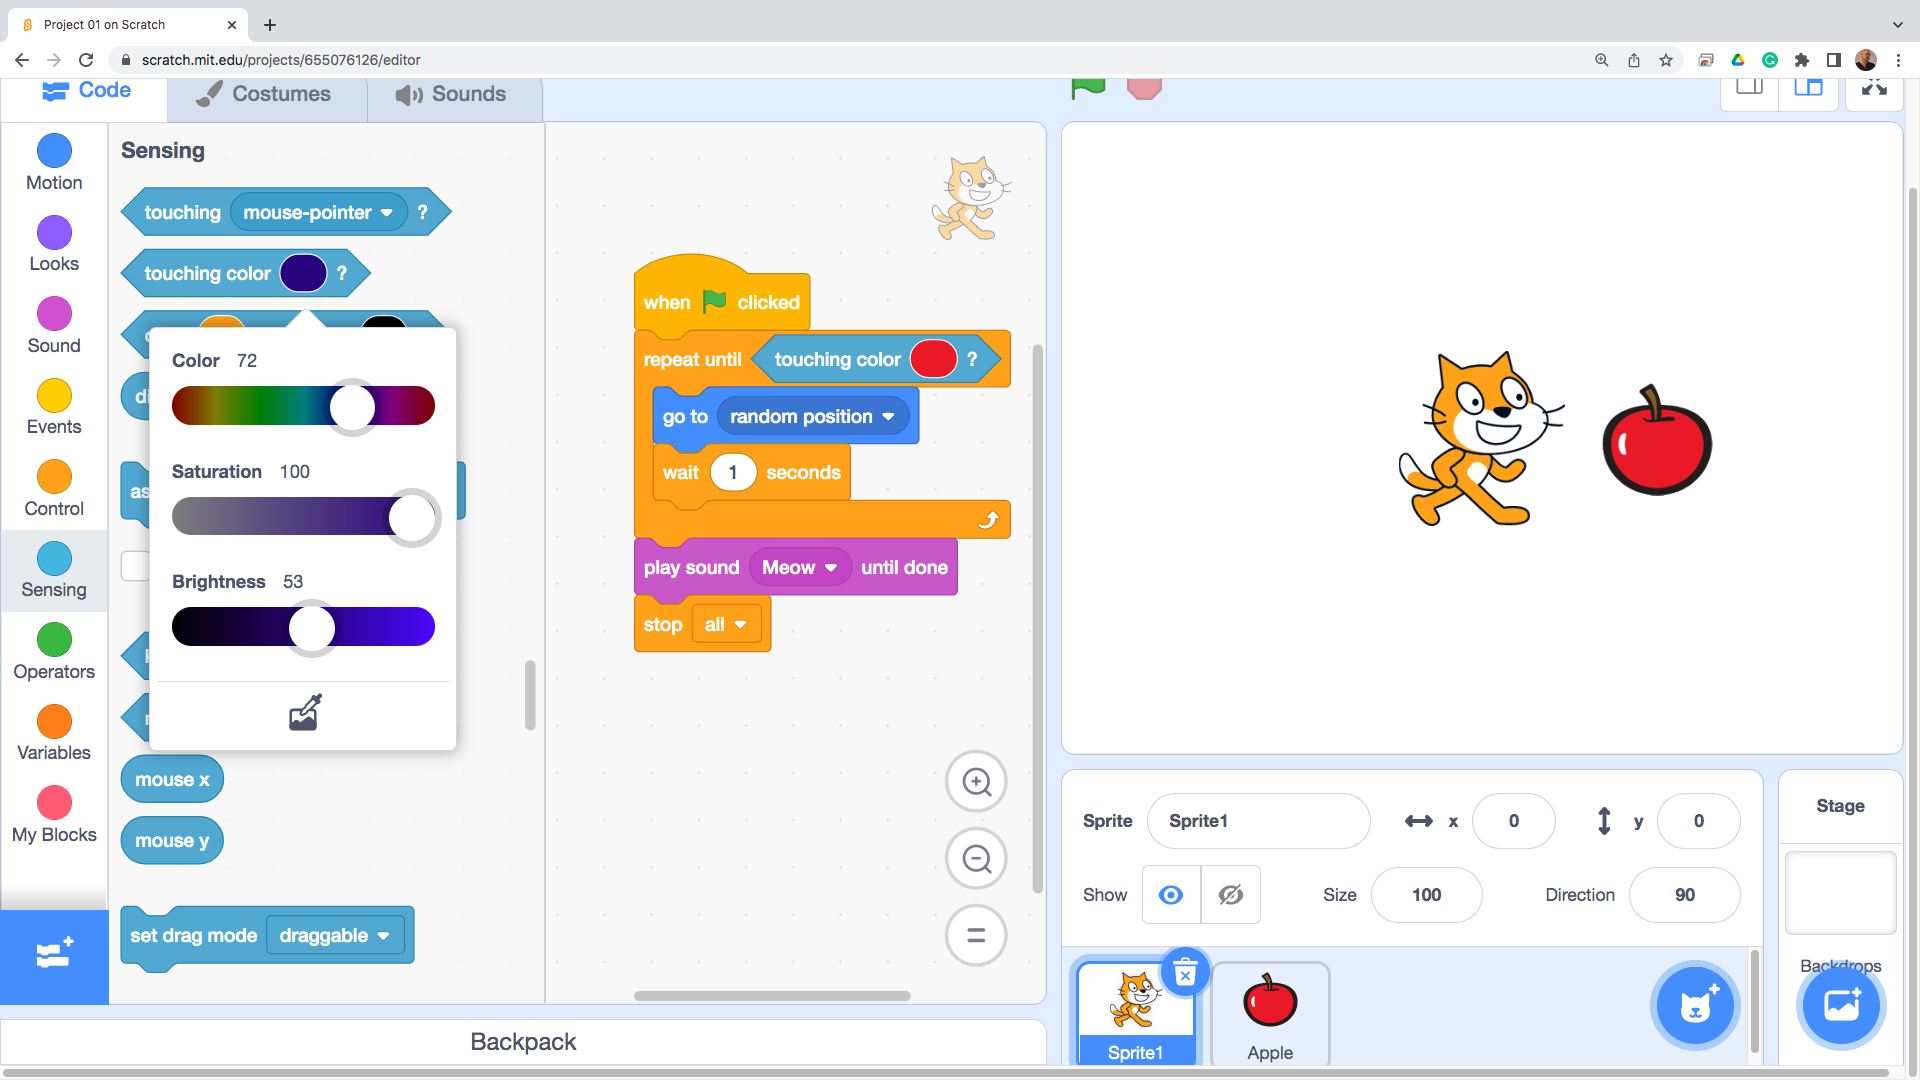
\includegraphics[width=1.0\linewidth,height=0.5\linewidth]{fig020045.png}
   \caption{Touch by Color}
\label{fig020045}
\end{figure}

With the previous block, no matter which part of the kitten touches the apple, the loop stops spinning, and the meow is heard. A much finer definition of collision between sprites can be obtained if only the black outline of the kitten is checked for touching the red color of the apple, which is what the next block is for (Fig. \ref{fig020046}).

\begin{figure}[H]
   \centering
   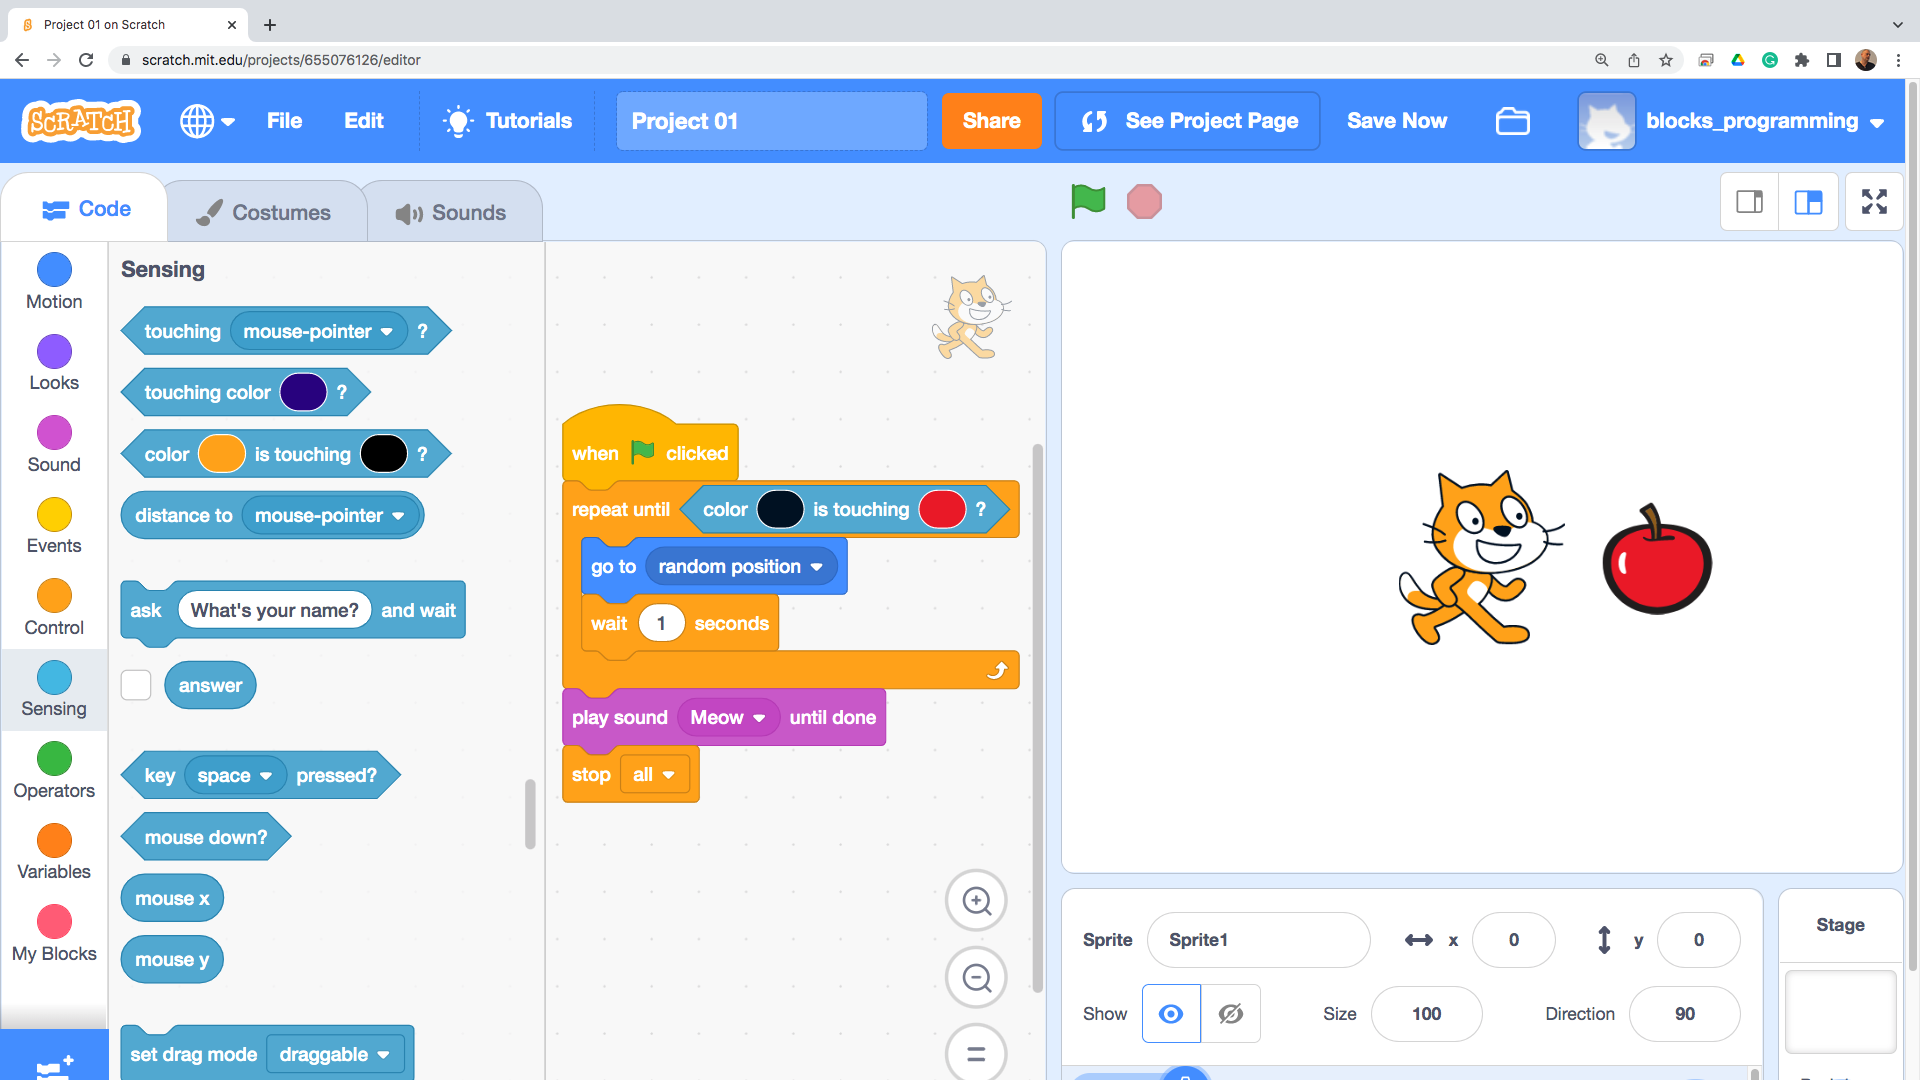
\includegraphics[width=1.0\linewidth,height=0.5\linewidth]{fig020046.png}
   \caption{Collision on two preset colors}
\label{fig020046}
\end{figure}

The next block is oval-shaped and supplies the program with the distance between the sprite and the mouse pointer. The oval shape suggests that this block should be embedded in one of the arithmetic expression blocks (Fig. \ref{fig020047}).

\begin{figure}[H]
   \centering
   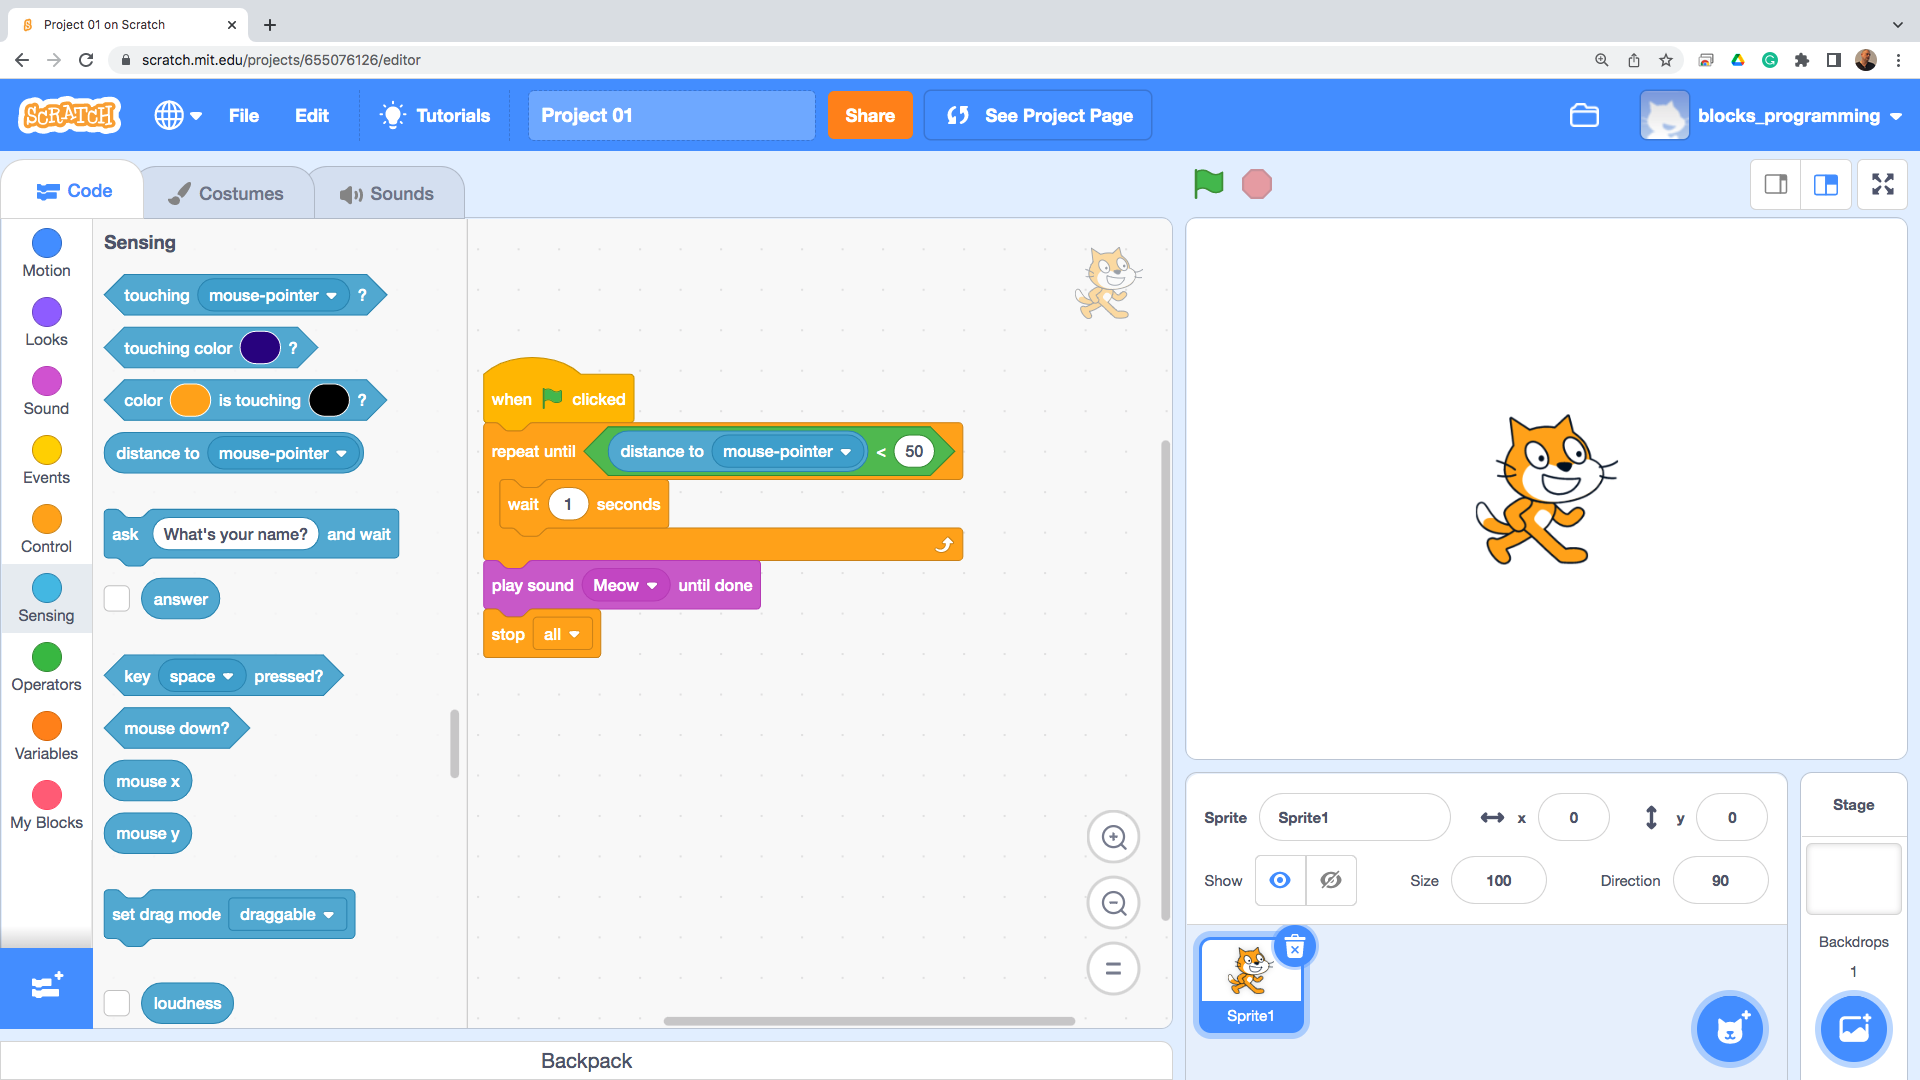
\includegraphics[width=1.0\linewidth,height=0.5\linewidth]{fig020047.png}
   \caption{Mouse Pointer Distance}
\label{fig020047}
\end{figure}

Sometimes the user needs to type something. To give this possibility is the next block in the light blue group (Fig. \ref{fig020048}). The animated character prompts the user by suggesting in specific text what is expected to be written.

\begin{figure}[H]
   \centering
   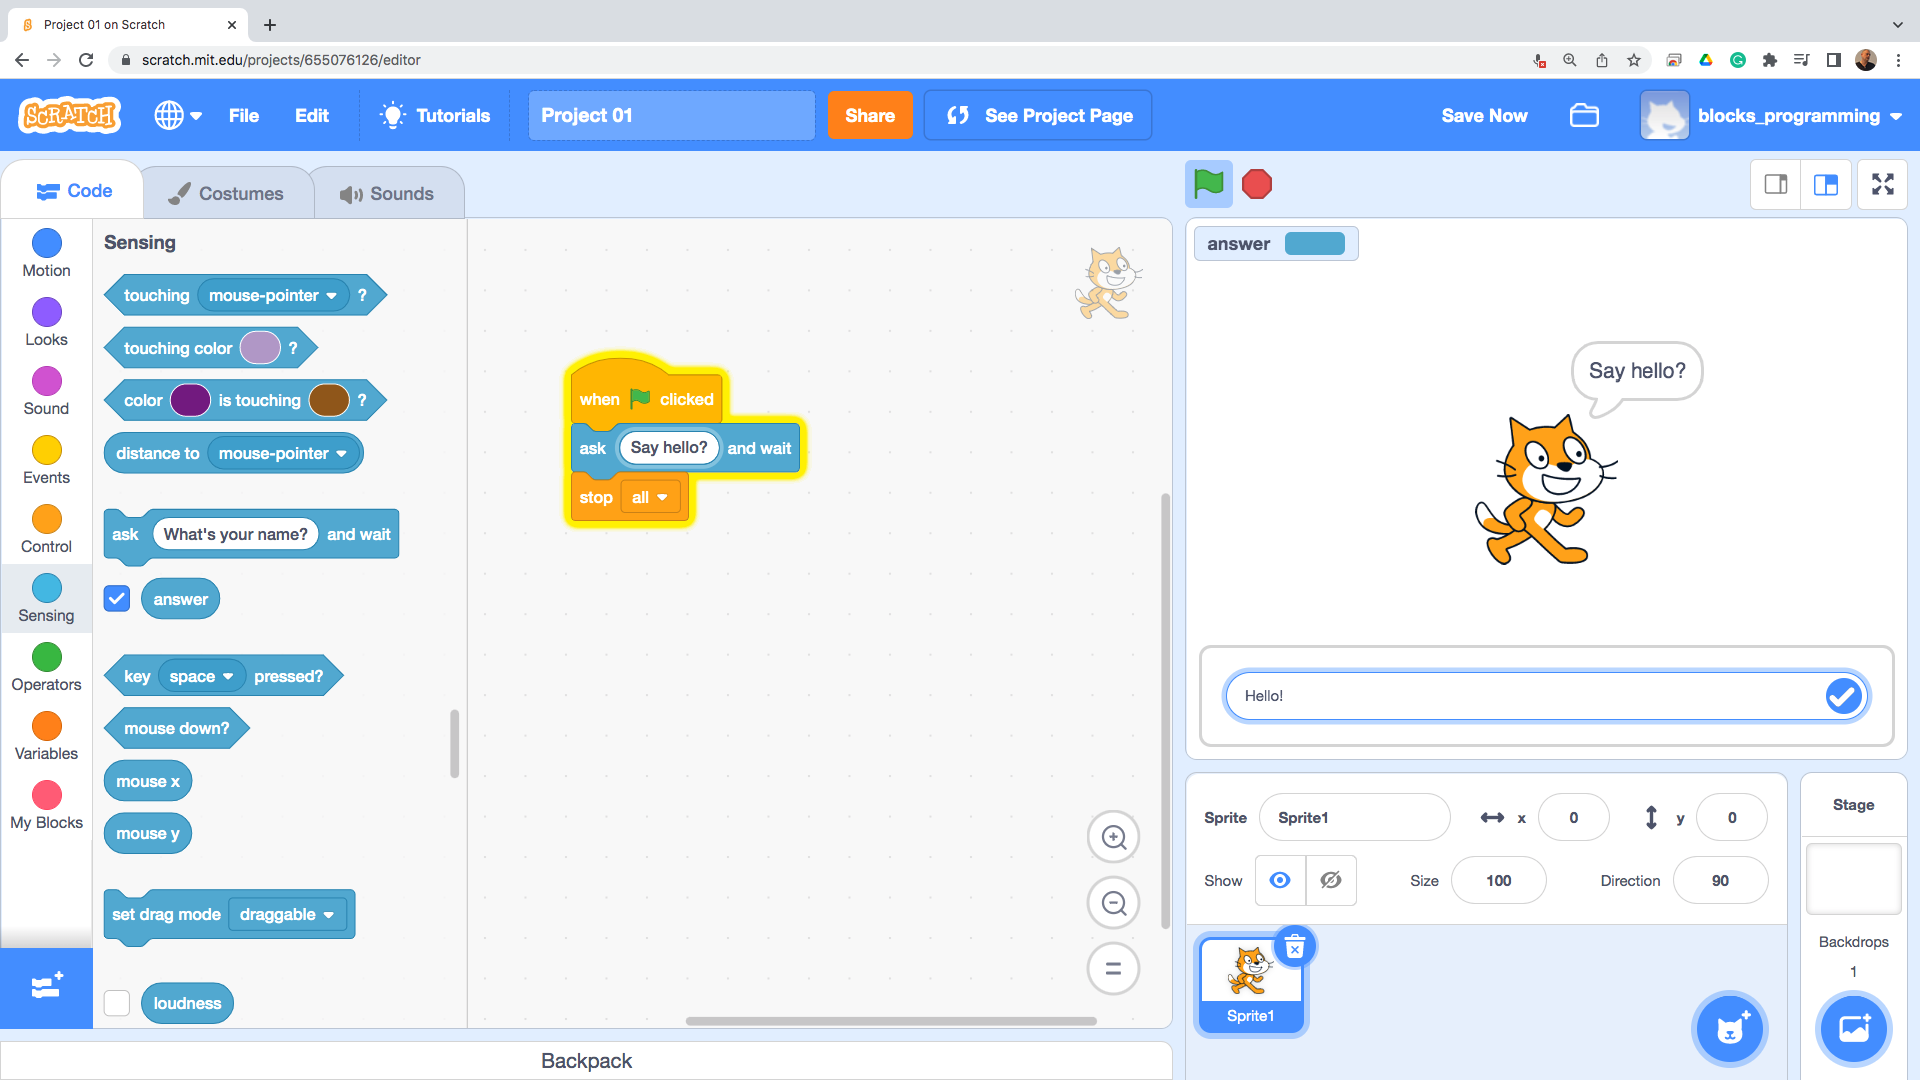
\includegraphics[width=1.0\linewidth,height=0.5\linewidth]{fig020048.png}
   \caption{Enter text}
\label{fig020048}
\end{figure}

The next block is one of the hexagonal blocks intended for embedding. This block returns a result of "true" when a particular key is pressed (Fig. \ref{fig020049}).

\begin{figure}[H]
   \centering
   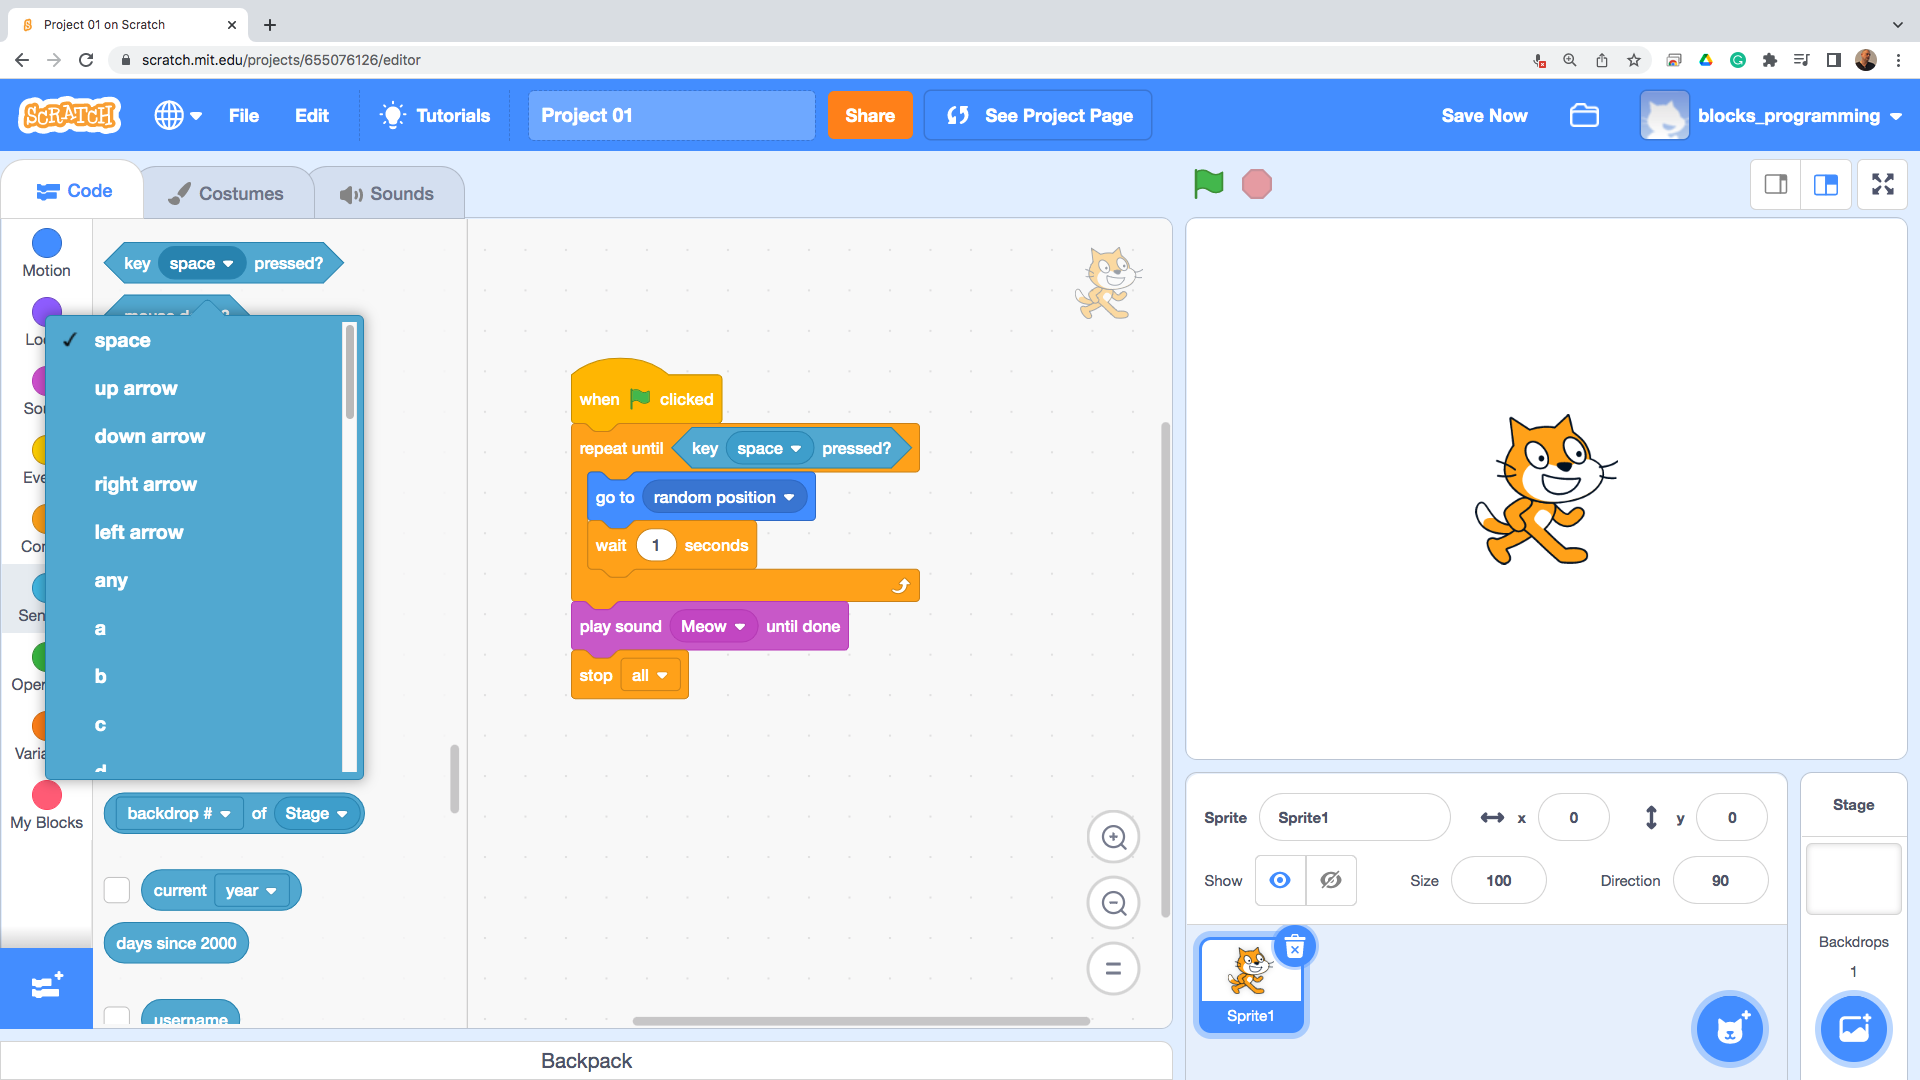
\includegraphics[width=1.0\linewidth,height=0.5\linewidth]{fig020049.png}
   \caption{Defining key pressed}
\label{fig020049}
\end{figure}

Similar behavior can be achieved with the next block, but a mouse key is expected instead of pressing a key on the keyboard (Fig. \ref{fig020050}).

\begin{figure}[H]
   \centering
   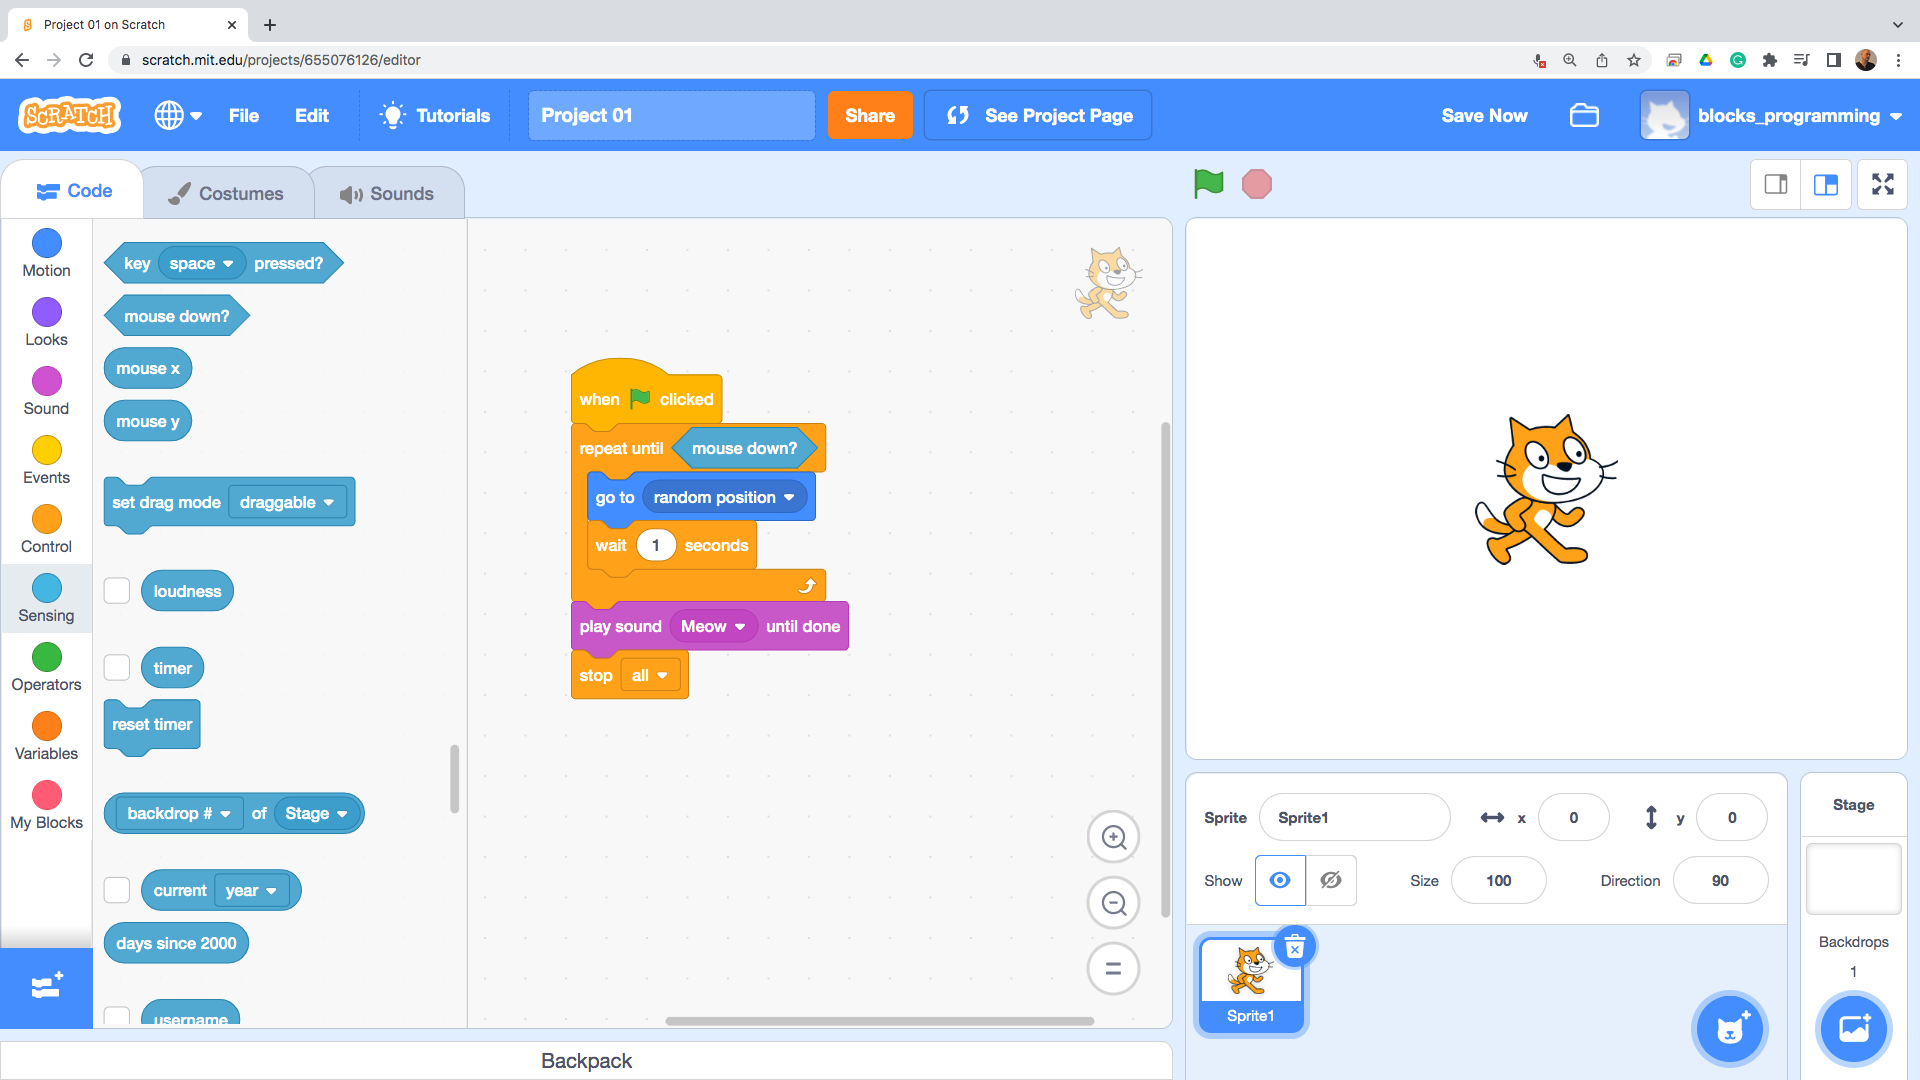
\includegraphics[width=1.0\linewidth,height=0.5\linewidth]{fig020050.png}
   \caption{Detect mouse button pressed}
\label{fig020050}
\end{figure}

The following two blocks are oval and are also for embedding. The first gives the coordinates of the animated character along the abscissa axis, and the second provides the coordinates of the animated character along the ordinate axis (Fig. \ref{fig020051}).

\begin{figure}[H]
   \centering
   \includegraphics[width=1.0\linewidth,height=0.5\linewidth]{fig020051.png}
   \caption{Coordinates of the animated character}
\label{fig020051}
\end{figure}

During the program operation, a functioning timer measures the time from the start of execution. With the next block, this timer can be reset (Fig. \ref{fig020052}).

\begin{figure}[H]
   \centering
   \includegraphics[width=1.0\linewidth,height=0.5\linewidth]{fig020052.png}
   \caption{Reset Timer}
\label{fig020052}
\end{figure}

The next block is one of the ovals, providing background information, variables, or sound level (Fig. \ref{fig020053}).

\begin{figure}[H]
   \centering
   \includegraphics[width=1.0\linewidth,height=0.5\linewidth]{fig020053.png}
   \caption{Scene Component Information}
\label{fig020053}
\end{figure}

The last block in the group is also intended for embedding and returns the number of days from the year 2000 (Fig. \ref{fig020054}).

\begin{figure}[H]
   \centering
   \includegraphics[width=1.0\linewidth,height=0.5\linewidth]{fig020054.png}
   \caption{Number of days since the beginning of the century}
\label{fig020054}
\end{figure}

The group of green blocks is intended for embedding. The first four blocks are oval and intended for arithmetic operations – addition, subtraction, multiplication, and division (Fig. \ref{fig020055}).

\begin{figure}[H]
   \centering
   \includegraphics[width=1.0\linewidth,height=0.5\linewidth]{fig020055.png}
   \caption{Arithmetic operations}
\label{fig020055}
\end{figure}

The random number block has already been demonstrated, but it fits perfectly into the three following blocks. These comparison blocks are intended to be embedded in the execution control blocks (Fig. \ref{fig020056}).

\begin{figure}[H]
   \centering
   \includegraphics[width=1.0\linewidth,height=0.5\linewidth]{fig020056.png}
   \caption{Comparison Operations}
\label{fig020056}
\end{figure}

Next are three hexagonal-shaped blocks (Fig. \ref{fig020057}), which serve to embed in control blocks. The three blocks perform the three basic logical operations ("and", "or", "not"). Both conditions must be met in the first block to enter the conditional transition construct. Precisely for this reason, the logical operation is called "and". One condition must be met in the second block to enter the conditional transition construct. For this reason, the logical operation is called "or". In the third block, the result is reversed, so the conditional transition construct is entered under a false condition. For this reason, this operation is called "negation".

\begin{figure}[H]
   \centering
   \includegraphics[width=1.0\linewidth,height=0.5\linewidth]{fig020057.png}
   \caption{Boolean operations}
\label{fig020057}
\end{figure}

The following four blocks are for working with character strings (Fig. \ref{fig020058}). The first three are oval in shape, and the last is hexagonal in form. The first block concatenates two character strings. The second block specifies a letter at a particular position in the character string. The third block specifies the length of the character string. The fourth block searches for a specific letter in the character string.

\begin{figure}[H]
   \centering
   \includegraphics[width=1.0\linewidth,height=0.5\linewidth]{fig020058.png}
   \caption{Working with character strings}
\label{fig020058}
\end{figure}

The last three blocks in the green group are intended for working with functions (Fig. \ref{fig020059}). The first block calculates the remainder of the integer division. The second block rounds a fractional number to its whole part. The third block offers the calculation of an entire list of mathematical functions.

\begin{figure}[H]
   \centering
   \includegraphics[width=1.0\linewidth,height=0.5\linewidth]{fig020059.png}
   \caption{Mathematical Functions}
\label{fig020059}
\end{figure}

The last group of blocks is the dark orange group (Fig. \ref{fig020060}). They are designed to work with variables. When writing programs, it is often necessary to save intermediate calculated results temporarily and use them for subsequent calculations. This is achieved through the variables. Variables are temporary containers that store their assigned values. The first block in the group establishes the variable's value. The second block in the group changes the variable's value. The third block in the group serves for program visualization of the variable. The last box in the group helps to hide the preview.

\begin{figure}[H]
   \centering
   \includegraphics[width=1.0\linewidth,height=0.5\linewidth]{fig020060.png}
   \caption{Working with variables}
\label{fig020060}
\end{figure}

Now that all the most important constructs in the Scratch programming environment have been introduced, one can move on to writing more complex programs, appropriately combining the basic building blocks.

\section{Programming Constructs in App Inventor}

A significant difference between App Inventor and Scratch is that App Inventor does not use sprites but builds a graphical user interface. This is because App Inventor takes a classic approach to writing Android apps. This difference makes it necessary to consider two types of expressions in App Inventor: the GUI components and the programming blocks for building a series of instructions.

Building an application in App Inventor starts on a new, blank screen (Fig. \ref{fig020061}). Screens are scenes, and the program's work moves from scene to scene. When the program is something straightforward, it can be realized as only one scene.

\begin{figure}[H]
   \centering
   \includegraphics[width=1.0\linewidth,height=0.5\linewidth]{fig020061.png}
   \caption{Opening Scene}
\label{fig020061}
\end{figure}

\subsection{Graphical Interface}

GUI components are organized into groups, just as instruction blocks are arranged. Most visual components have a graphical layout directly on the screen, but some are not visualized. An example of non-renderable components is layout management managers. These managers are represented in the second group, and their function is to serve as grouping components that arrange the visually presented components.

A hierarchical structure of the positioned graphic components is presented on the right of the working scene. Components can be deleted or renamed in this panel. On the far right is a panel with the characteristics of the currently selected graphic component. Components have different features, which can be established while designing the interface.

The first group includes the main components for building a graphical user interface. The first component in this group is the button (Fig. \ref{fig020062}). Placing it in the workspace of the scene is done by selecting with the mouse and dragging it to the workspace. The button has characteristics related to the text on the component itself, the ability to place an image, dimensions, shape, font size, background, and foreground colors, and others.

\begin{figure}[H]
   \centering
   \includegraphics[width=1.0\linewidth,height=0.5\linewidth]{fig020062.png}
   \caption{Button Graphical Component}
\label{fig020062}
\end{figure}

The button is followed by a marking component (Fig. \ref{fig020063}), which has similar functionality to the button, but the on or off state is marked. It is often used to denote properties. The most important characteristic of this component is whether it is in the established state or in the disabled state.

\begin{figure}[H]
   \centering
   \includegraphics[width=1.0\linewidth,height=0.5\linewidth]{fig020063.png}
   \caption{Graphical ticker component}
\label{fig020063}
\end{figure}

Entering dates by the user is a process that can lead to many errors. This is because different months have different lengths, and the month of February is determined by leap years and whether the corresponding leap year is a multiple of four hundred. To avoid date entry errors, Android offers a visual component for controlled date entry (Fig. \ref{fig020064}).

\begin{figure}[H]
   \centering
   \includegraphics[width=1.0\linewidth,height=0.5\linewidth]{fig020064.png}
   \caption{Graphic component for entering dates}
\label{fig020064}
\end{figure}

The date input component may have a different presentation in different versions or proprietary modifications of the Android operating system. One possibility is a counter with three segments for day, month, and year (Fig. \ref{fig020065}).

\begin{figure}[H]
   \centering
   \includegraphics[width=1.0\linewidth,height=0.5\linewidth]{fig020065.png}
   \caption{Enter date}
\label{fig020065}
\end{figure}

The following visual component has the sole task of displaying an image (Fig. \ref{fig020066}). This is also the most essential characteristic in the characteristics panel for the component.

\begin{figure}[H]
   \centering
   \includegraphics[width=1.0\linewidth,height=0.5\linewidth]{fig020066.png}
   \caption{Graphic component for images}
\label{fig020066}
\end{figure}

Next is the label, a text field with no possibility for the user to change the text content (Fig. \ref{fig020067}).

\begin{figure}[H]
   \centering
   \includegraphics[width=1.0\linewidth,height=0.5\linewidth]{fig020067.png}
   \caption{Label Graphical Component}
\label{fig020067}
\end{figure}

In the next component, selecting from a list of character strings is possible. A comma is used as a separator between strings (Fig. \ref{fig020068}).

\begin{figure}[H]
   \centering
   \includegraphics[width=1.0\linewidth,height=0.5\linewidth]{fig020068.png}
   \caption{Selectable Graphical Component}
\label{fig020068}
\end{figure}

Each option is visualized on a separate line (Fig. \ref{fig020069}).

\begin{figure}[H]
   \centering
   \includegraphics[width=1.0\linewidth,height=0.5\linewidth]{fig020069.png}
   \caption{List options}
\label{fig020069}
\end{figure}

In the list view component, a separate cell is provided for each option (Fig. \ref{fig020070}).

\begin{figure}[H]
   \centering
   \includegraphics[width=1.0\linewidth,height=0.5\linewidth]{fig020070.png}
   \caption{List widget}
\label{fig020070}
\end{figure}

The next component is one of the components that need to be visualized at design time. Used to display notifications (Fig. \ref{fig020071}).

\begin{figure}[H]
   \centering
   \includegraphics[width=1.0\linewidth,height=0.5\linewidth]{fig020071.png}
   \caption{Notification widget}
\label{fig020071}
\end{figure}

To be visualized, it is necessary to add several instructions to the intercepted event so that during execution, the written texts are displayed (Fig. \ref{fig020072}). The interception is for the back button pressed event when the app shows the first scene.

\begin{figure}[H]
   \centering
   \includegraphics[width=1.0\linewidth,height=0.5\linewidth]{fig020072.png}
   \caption{A series of instructions to display a notification}
\label{fig020072}
\end{figure}

During the preview, the popup dialog can be dismissed (Fig. \ref{fig020073}) because the cancel option is enabled.

\begin{figure}[H]
   \centering
   \includegraphics[width=1.0\linewidth,height=0.5\linewidth]{fig020073.png}
   \caption{Notification window}
\label{fig020073}
\end{figure}

Password input fields look like regular text input fields, but the difference is that when typing, the characters are not visible but are replaced by asterisks (Fig. \ref{fig020074}).

\begin{figure}[H]
   \centering
   \includegraphics[width=1.0\linewidth,height=0.5\linewidth]{fig020074.png}
   \caption{Graphical component for entering passwords}
\label{fig020074}
\end{figure}

With a slider component, the two most important characteristics are the minimum and maximum values that the component can take. The slider serves to visualize a position on a linear scale (Fig. \ref{fig020075}).

\begin{figure}[H]
   \centering
   \includegraphics[width=1.0\linewidth,height=0.5\linewidth]{fig020075.png}
   \caption{Position Graphical Component}
\label{fig020075}
\end{figure}

At the next component, choices are given, again as an enumerated list of character strings (Fig. \ref{fig020076}).

\begin{figure}[H]
   \centering
   \includegraphics[width=1.0\linewidth,height=0.5\linewidth]{fig020076.png}
   \caption{Selectable Graphical Component}
\label{fig020076}
\end{figure}

The options' visual presentation differs from those presented in the previous components (Fig. \ref{fig020077}).

\begin{figure}[H]
   \centering
   \includegraphics[width=1.0\linewidth,height=0.5\linewidth]{fig020077.png}
   \caption{Selection via radio buttons}
\label{fig020077}
\end{figure}

The key type component is an alternative to the check box component (Fig. \ref{fig020078}). The most important characteristic of this component is the state it is in - on or off.

\begin{figure}[H]
   \centering
   \includegraphics[width=1.0\linewidth,height=0.5\linewidth]{fig020078.png}
   \caption{Switch widget}
\label{fig020078}
\end{figure}

The text field is a component that enters text from the user (Fig. \ref{fig020079}).

\begin{figure}[H]
   \centering
   \includegraphics[width=1.0\linewidth,height=0.5\linewidth]{fig020079.png}
   \caption{Text input widget}
\label{fig020079}
\end{figure}

By analogy with the date input component, a time input component is also available (Fig. \ref{fig020080}).

\begin{figure}[H]
   \centering
   \includegraphics[width=1.0\linewidth,height=0.5\linewidth]{fig020080.png}
   \caption{Time input widget}
\label{fig020080}
\end{figure}

One of its possible implementations takes the form of three fields, two for scrolling up/down and one for specifying morning or afternoon (Fig. \ref{fig020081}).

\begin{figure}[H]
   \centering
   \includegraphics[width=1.0\linewidth,height=0.5\linewidth]{fig020081.png}
   \caption{Choose a time}
\label{fig020081}
\end{figure}

The most feature-rich component is the last in the group and is an entire web browser (Fig. \ref{fig020082}).

\begin{figure}[H]
   \centering
   \includegraphics[width=1.0\linewidth,height=0.5\linewidth]{fig020082.png}
   \caption{Web Browser Graphical Component}
\label{fig020082}
\end{figure}

Entire web pages (Fig. \ref{fig020083}) can be loaded into this component, including those that require JavaScript interactivity.

\begin{figure}[H]
   \centering
   \includegraphics[width=1.0\linewidth,height=0.5\linewidth]{fig020083.png}
   \caption{Loading Web Page}
\label{fig020083}
\end{figure}

The second group of visual components organizes the graphical user interface and are containers for the components with a visual representation. This mechanism for managing the graphical user interface was proposed with the first graphic user interface libraries offered with the Java programming language. This organization aims to make the graphical user interface suitable for devices with different screen sizes. Visual components are arranged according to the available area and the containers' rules.

With the first component in the group, the visual components are arranged horizontally, hence its name (Fig. \ref{fig020084}).

\begin{figure}[H]
   \centering
   \includegraphics[width=1.0\linewidth,height=0.5\linewidth]{fig020084.png}
   \caption{Horizontal stacking container}
\label{fig020084}
\end{figure}

In the first container, if the visual components go outside the user's visible field of operation, they cannot be reached. For this reason, the second container provides scrolling capabilities (horizontally) so that visual components that go outside the work area can be reached (Fig. \ref{fig020085}).

\begin{figure}[H]
   \centering
   \includegraphics[width=1.0\linewidth,height=0.5\linewidth]{fig020085.png}
   \caption{Horizontal stacking container with slider}
\label{fig020085}
\end{figure}

The third container in the group allows the visual components to be arranged as a table with rows and columns (Fig. \ref{fig020086}).

\begin{figure}[H]
   \centering
   \includegraphics[width=1.0\linewidth,height=0.5\linewidth]{fig020086.png}
   \caption{Table arrangement container}
\label{fig020086}
\end{figure}

By analogy with the container for horizontal stacking, a container for vertical stacking is also provided (Fig. \ref{fig020087}). In it, visual components are stacked on top of each other.

\begin{figure}[H]
   \centering
   \includegraphics[width=1.0\linewidth,height=0.5\linewidth]{fig020087.png}
   \caption{Vertical stack container}
\label{fig020087}
\end{figure}

In case of insufficient working space along the vertical axis, it is also possible to use a container with the possibility of sliding (Fig. \ref{fig020088}).

\begin{figure}[H]
   \centering
   \includegraphics[width=1.0\linewidth,height=0.5\linewidth]{fig020088.png}
   \caption{Vertical stacking container with slider}
\label{fig020088}
\end{figure}

The slider appears on the container's borders but disappears when there is no sliding, so it only takes up a little visual space (Fig. ef {fig020089}).

\begin{figure}[H]
   \centering
   \includegraphics[width=1.0\linewidth,height=0.5\linewidth]{fig020089.png}
   \caption{Slide content into container}
\label{fig020089}
\end{figure}

A significant advantage of containers is that they can be nested within other containers (Fig. \ref{fig020090}). By appropriately arranging the different embeddings, a graphical user interface layout that looks good on devices with different screen sizes can be achieved.

\begin{figure}[H]
   \centering
   \includegraphics[width=1.0\linewidth,height=0.5\linewidth]{fig020090.png}
   \caption{Inserting containers}
\label{fig020090}
\end{figure}

There is a multimedia group after the component group is used to arrange the visible components. In this group, components have no graphical representation at design time but no visual representation at runtime. Two components are an exception. The first is an image selection component, and the second is a video display component (Fig. \ref{fig020091}).

\begin{figure}[H]
   \centering
   \includegraphics[width=1.0\linewidth,height=0.5\linewidth]{fig020091.png}
   \caption{Multimedia Group}
\label{fig020091}
\end{figure}

The group of multimedia components provides programming capabilities to perform specific tasks: video recording, photo recording, sound file playback, sound management, sound file recording, speech recognition, speech synthesis, and machine translation between spoken languages. The complexity of the components in this group prevents their easy demonstration, but some of them will be used in the following examples.

After the multimedia group comes the animation group (Fig. \ref{fig020092}). When writing games, the concept of the canvas (Canvas) and moving animated characters (Sprites) are often used. The familiar Scratch sprites appear here, too, but in an exceptional case.

\begin{figure}[H]
   \centering
   \includegraphics[width=1.0\linewidth,height=0.5\linewidth]{fig020092.png}
   \caption{Animation Group}
\label{fig020092}
\end{figure}

Generally, a canvas is a two-dimensional matrix of colored dots (pixels) on which various two-dimensional primitives or bitmaps with a transparency channel are drawn. It is important to note that sprites cannot be placed independently but must be below the canvas hierarchy.

Since the Android operating system is primarily implemented on mobile devices, and they very often have GPS sensors, the next group of components provides opportunities for working with geographic maps and geolocation (Fig. \ref{fig020093}).

\begin{figure}[H]
   \centering
   \includegraphics[width=1.0\linewidth,height=0.5\linewidth]{fig020093.png}
   \caption{Geolocation Group}
\label{fig020093}
\end{figure}

Analogous to the drawing canvas, this group also has a primary map visualization component, which can contain graphic primitives such as circles, feature selection, lines, markers, polygons, and rectangles. There is also a component that does not have a preview but serves to enable map navigation functionality. Map rendering is done in layers, which allows graphics primitives to be added above the map rendering layer itself.

Different mobile devices have different set of hardware sensors (Fig. \ref{fig020094}). Sensors are parts of the device that collect information from the external environment. In the next group of components, it is possible to program work with different types of sensors, such as an accelerometer, barcode reader, pressure sensor, clock, spatial orientation sensor, humidity sensor, illumination sensor, a location sensor, magnetic field strength, proximity sensor, spatial orientation sensor, pedometer, object proximity sensor, and thermometer.

\begin{figure}[H]
   \centering
   \includegraphics[width=1.0\linewidth,height=0.5\linewidth]{fig020094.png}
   \caption{Sensor Working Group}
\label{fig020094}
\end{figure}

All components in the group have no visual representation and are used through program constructs. Working with the hardware and its sensors requires considerable skill and is beyond the scope of this presentation.

The next group presents components that are related to social contacts. The first component allows the selection of a person from the contact list (Fig. \ref{fig020095}). The contact list saves information about various people with whom the user communicates.

\begin{figure}[H]
   \centering
   \includegraphics[width=1.0\linewidth,height=0.5\linewidth]{fig020095.png}
   \caption{Contact Selector Graphical Component}
\label{fig020095}
\end{figure}

Next is a component for entering an e-mail address (Fig. \ref{fig020096}). E-mail addresses have a strictly fixed format, which must be followed when the user enters.

\begin{figure}[H]
   \centering
   \includegraphics[width=1.0\linewidth,height=0.5\linewidth]{fig020096.png}
   \caption{Email input widget}
\label{fig020096}
\end{figure}

The phone call initiation component is for programmatic use and has no visual representation (Fig. \ref{fig020097}).

\begin{figure}[H]
   \centering
   \includegraphics[width=1.0\linewidth,height=0.5\linewidth]{fig020097.png}
   \caption{Phone Call Component}
\label{fig020097}
\end{figure}

Next is a component for selecting a phone number from the contact list (Fig. \ref{fig020098}).

\begin{figure}[H]
   \centering
   \includegraphics[width=1.0\linewidth,height=0.5\linewidth]{fig020098.png}
   \caption{Graphic component for selecting a phone number}
\label{fig020098}
\end{figure}

The last three components have no visual representation and serve to share information, send text messages, and post to Twitter (Fig. \ref{fig020099}). These components are intended for programmatic use only and enable applications within the operating system.

\begin{figure}[H]
   \centering
   \includegraphics[width=1.0\linewidth,height=0.5\linewidth]{fig020099.png}
   \caption{Information Sharing Component}
\label{fig020099}
\end{figure}

Next is a group of components without visual representation. This group has the task of storing the information between separate program starts (Fig. \ref{fig020100}). The first component stores the information on a remote cloud service. An address to the remote server is provided for this purpose. The second component serves to work with files on the local drive. The third component serves to store structured information between separate program launches. The storage is on the local drive and can be likened to variables saved after the program is stopped. Using the web services mechanism, the latter component stores information on a remote server.

\begin{figure}[H]
   \centering
   \includegraphics[width=1.0\linewidth,height=0.5\linewidth]{fig020100.png}
   \caption{Information storage component}
\label{fig020100}
\end{figure}

The next group of components is responsible for communication connectivity (Fig. \ref{fig020101}). All components have no visual representation and are intended for programmatic use. The first component is used to open the next screen, the way it happens in Android programs. The second component adds client-side Bluetooth functionality. The third component adds server-side Bluetooth functionality. The fourth component enables serial communication with devices such as Arduino. The last component in the group allows web-based communication without rendering, as is the case with the web browser component.

\begin{figure}[H]
   \centering
   \includegraphics[width=1.0\linewidth,height=0.5\linewidth]{fig020101.png}
   \caption{Communication Connectivity Component}
\label{fig020101}
\end{figure}

One of the largest groups of components is for working with Lego Mindstorms (Fig. \ref{fig020102}). This series from the Lego company is designed for children interested in robotics. Ince the topic of robotics falls outside the scope of this presentation, these components will not be discussed.

\begin{figure}[H]
   \centering
   \includegraphics[width=1.0\linewidth,height=0.5\linewidth]{fig020102.png}
   \caption{Lego Mindstorms Component}
\label{fig020102}
\end{figure}

The group of experimental components includes only a component for working with a Firebase database (Fig. \ref{fig020103}).

\begin{figure}[H]
   \centering
   \includegraphics[width=1.0\linewidth,height=0.5\linewidth]{fig020103.png}
   \caption{Experimental Components}
\label{fig020103}
\end{figure}

The graphical user interface in the Android operating system is designed so that third-party manufacturers of visual components can add them in the form of libraries. This option is also available in App Inventor as the last group in the component groups panel.

\subsection{Program Constructs}

Unlike Scratch, App Inventor has many more blocks, as each GUI component has multiple event-handling capabilities and accordingly offers slots for nesting block constructs. For this reason, only the main blocks will be considered, and the rest will be partially demonstrated in the subsequent exposition.

Basic blocks in App Inventor have identical functionality to blocks in Scratch. Visually, they are shaped differently, but the idea is the same – the blocks follow or are built into each other. For the demonstration of most blocks, one button and one instance of the notification component will be used (Fig. \ref{fig020104}). The button press event is the ideal slot to place the demonstrated constructs.

\begin{figure}[H]
   \centering
   \includegraphics[width=1.0\linewidth,height=0.5\linewidth]{fig020104.png}
   \caption{A minimal interface for demonstrating block constructions}
\label{fig020104}
\end{figure}

The block constructions are also arranged in a workspace specially set aside for this purpose (Fig. \ref{fig020105}).

\begin{figure}[H]
   \centering
   \includegraphics[width=1.0\linewidth,height=0.5\linewidth]{fig020105.png}
   \caption{Workspace for block structures}
\label{fig020105}
\end{figure}

The blocks are again organized into colored groups, which will be arranged in the button-pressed event slot (Fig. \ref{fig020106}).

\begin{figure}[H]
   \centering
   \includegraphics[width=1.0\linewidth,height=0.5\linewidth]{fig020106.png}
   \caption{Groups of colored blocks}
\label{fig020106}
\end{figure}

First is the colored group of brown blocks, which controls the performance. It starts with the familiar conditional transition block (Fig. \ref{fig020107}).

\begin{figure}[H]
   \centering
   \includegraphics[width=1.0\linewidth,height=0.5\linewidth]{fig020107.png}
   \caption{Conditional transition block}
\label{fig020107}
\end{figure}

If the condition in the transition construct evaluates to true, then a notification display is called in the block's body by embedding a purple block (Fig. \ref{fig020108}) from the list of blocks in the notifications component.

\begin{figure}[H]
   \centering
   \includegraphics[width=1.0\linewidth,height=0.5\linewidth]{fig020108.png}
   \caption{View Notification}
\label{fig020108}
\end{figure}

The bolded text of the notification is written in a magenta block and embedded in the notification preview block (Fig. \ref{fig020109}).

\begin{figure}[H]
   \centering
   \includegraphics[width=1.0\linewidth,height=0.5\linewidth]{fig020109.png}
   \caption{Notification text}
\label{fig020109}
\end{figure}

Next is the formation of the header part of the conditional transition construction. A blue block is placed next to the title slot, where the transition condition will be entered (Fig. \ref{fig020110}).

\begin{figure}[H]
   \centering
   \includegraphics[width=1.0\linewidth,height=0.5\linewidth]{fig020110.png}
   \caption{Transition block header}
\label{fig020110}
\end{figure}

A blue box on the left side of the condition expression generates a random number in a set interval (Fig. \ref{fig020111}).

\begin{figure}[H]
   \centering
   \includegraphics[width=1.0\linewidth,height=0.5\linewidth]{fig020111.png}
   \caption{Left side of condition expression}
\label{fig020111}
\end{figure}

On the right side in the condition, there is a blue block with an exact predefined value (Fig. \ref{fig020112}). That way, the caption will be displayed on some button presses, and on others, it won't.

\begin{figure}[H]
   \centering
   \includegraphics[width=1.0\linewidth,height=0.5\linewidth]{fig020112.png}
   \caption{Right side of condition expression}
\label{fig020112}
\end{figure}

When the random number is below the set threshold, the notification is displayed for a short interval and then disappears (Fig. \ref{fig020113}).

\begin{figure}[H]
   \centering
   \includegraphics[width=1.0\linewidth,height=0.5\linewidth]{fig020113.png}
   \caption{Notification Preview}
\label{fig020113}
\end{figure}

The second block in the brown group is for a conditional transition, executing a block construction when the condition is met but another construction when the condition is not (Fig. \ref{fig020114}).

\begin{figure}[H]
   \centering
   \includegraphics[width=1.0\linewidth,height=0.5\linewidth]{fig020114.png}
   \caption{Conditional transition block and alternative}
\label{fig020114}
\end{figure}

The third block in the brown group represents a cascade for conditional transitions (Fig. \ref{fig020115}). More than one condition is checked.

\begin{figure}[H]
   \centering
   \includegraphics[width=1.0\linewidth,height=0.5\linewidth]{fig020115.png}
   \caption{Conditional transition cascade block}
\label{fig020115}
\end{figure}

The next block in the brown group is a step loop block (Fig. \ref{fig020116}). The variable's value is taken via an orange block at each loop turn and displayed as a notification.

\begin{figure}[H]
   \centering
   \includegraphics[width=1.0\linewidth,height=0.5\linewidth]{fig020116.png}
   \caption{Step loop block}
\label{fig020116}
\end{figure}

The next block in the brown group is for looping over the elements of a list structure (Fig. \ref{fig020117}). The purple block is handy for forming a list, which divides a character string into substrings according to a predefined delimiter.

\begin{figure}[H]
   \centering
   \includegraphics[width=1.0\linewidth,height=0.5\linewidth]{fig020117.png}
   \caption{List loop block}
\label{fig020117}
\end{figure}

Next is a block in the brown group to loop over the elements of a "dictionary" type structure (Fig. \ref{fig020118}). This type of structure is also known as an "associative array". To access the elements, the key value does not have to be a number but can be a character string, for example. The key is used to access the items. A dark blue block is used to create the dictionary. Some blocks have a small gear in the upper left corner. This wheel is an icon that expands to a block setting menu. In this case, the number of slots for key-value pairs is determined through the setting. The orange blocks take the contents of the two variables local to the loop. One variable contains the key, and the other contains the value corresponding to that key. A purple string concatenation block forms the text message displayed in the notification component.

\begin{figure}[H]
   \centering
   \includegraphics[width=1.0\linewidth,height=0.5\linewidth]{fig020118.png}
   \caption{Vocabulary loop block}
\label{fig020118}
\end{figure}

The next block implements a loop with a precondition of type "while" (Fig. \ref{fig020119}). In this loop, the iteration termination condition precedes the loop body. For execution control, creating an external variable via an orange variable initialization block is necessary. In this case, the variable is initialized with a random value. In the loop header, a check is made for the variable's value, and a decision is made on whether the loop should continue running. The variable's value is visualized in the notifications component, and then, with an appropriate orange block, a new random value is selected. The loop stops spinning when the value in the variable drops below the preset threshold.

\begin{figure}[H]
   \centering
   \includegraphics[width=1.0\linewidth,height=0.5\linewidth]{fig020119.png}
   \caption{For loop block with precondition}
\label{fig020119}
\end{figure}

The next block has the meaning of a ternary operation in the Java programming language and resembles the conditional transition construction with an alternative (Fig. \ref{fig020120}). If the condition evaluates to true, the result returned is the first possibility. If it evaluates to "false", the result returned is the second possibility.

\begin{figure}[H]
   \centering
   \includegraphics[width=1.0\linewidth,height=0.5\linewidth]{fig020120.png}
   \caption{Ternary operation block}
\label{fig020120}
\end{figure}

The next block executes a series of other blocks and returns a result (Fig. \ref{fig020121}). This case uses a blue block that generates a random fractional number in the range of zero to one without including the unit.

\begin{figure}[H]
   \centering
   \includegraphics[width=1.0\linewidth,height=0.5\linewidth]{fig020121.png}
   \caption{Instruction grouping block}
\label{fig020121}
\end{figure}

The next block executes the instructions attached to it but ignores the resulting result (Fig. \ref{fig020122}). This block is useful when calling a function that returns a result, but the result is unnecessary.

\begin{figure}[H]
   \centering
   \includegraphics[width=1.0\linewidth,height=0.5\linewidth]{fig020122.png}
   \caption{Block to execute instructions with no result}
\label{fig020122}
\end{figure}

The next block opens a new screen (Fig. \ref{fig020123}); for this purpose, a second screen must be added to the project.

\begin{figure}[H]
   \centering
   \includegraphics[width=1.0\linewidth,height=0.5\linewidth]{fig020123.png}
   \caption{Open new screen block}
\label{fig020123}
\end{figure}

The new screen should be given a service name (Fig. \ref{fig020124}). Each screen has its own set of visual components and its own set of program constructs.

\begin{figure}[H]
   \centering
   \includegraphics[width=1.0\linewidth,height=0.5\linewidth]{fig020124.png}
   \caption{Screen Naming}
\label{fig020124}
\end{figure}

The second screen uses the same concept: one button and one notification component (Fig. \ref{fig020125}).

\begin{figure}[H]
   \centering
   \includegraphics[width=1.0\linewidth,height=0.5\linewidth]{fig020125.png}
   \caption{Second screen user interface}
\label{fig020125}
\end{figure}

In the initialization event of the second screen, the text is displayed by using the notification component in the second screen (Fig. \ref{fig020126}).

\begin{figure}[H]
   \centering
   \includegraphics[width=1.0\linewidth,height=0.5\linewidth]{fig020126.png}
   \caption{Notification when opening the second screen}
\label{fig020126}
\end{figure}

The next block opens a new screen, passing a value to the newly opened screen (Fig. \ref{fig020127}).

\begin{figure}[H]
   \centering
   \includegraphics[width=1.0\linewidth,height=0.5\linewidth]{fig020127.png}
   \caption{Open parameter passing screen}
\label{fig020127}
\end{figure}

The next block takes the value with which the screen was started (Fig. \ref{fig020128}).

\begin{figure}[H]
   \centering
   \includegraphics[width=1.0\linewidth,height=0.5\linewidth]{fig020128.png}
   \caption{Value the screen is started with}
\label{fig020128}
\end{figure}

The next block closes the screen (Fig. \ref{fig020129}). In this case, the closing is performed when the button is pressed on the second screen.

\begin{figure}[H]
   \centering
   \includegraphics[width=1.0\linewidth,height=0.5\linewidth]{fig020129.png}
   \caption{Screen close block}
\label{fig020129}
\end{figure}

The next block closes the screen, returning a result (Fig. \ref{fig020130}). The different screens can exchange information using the startup value and the returned slenderness.

\begin{figure}[H]
   \centering
   \includegraphics[width=1.0\linewidth,height=0.5\linewidth]{fig020130.png}
   \caption{Screen close block with return value}
\label{fig020130}
\end{figure}

The next block closes the entire program (Fig. \ref{fig020131}).

\begin{figure}[H]
   \centering
   \includegraphics[width=1.0\linewidth,height=0.5\linewidth]{fig020131.png}
   \caption{Program close block}
\label{fig020131}
\end{figure}

The next block gives the starting value as text (Fig. \ref{fig020132}).

\begin{figure}[H]
   \centering
   \includegraphics[width=1.0\linewidth,height=0.5\linewidth]{fig020132.png}
   \caption{Text of the value with which the screen is started}
\label{fig020132}
\end{figure}

With the next block, the screen is closed, and text is sent as the return value (Fig. \ref{fig020133}).

\begin{figure}[H]
   \centering
   \includegraphics[width=1.0\linewidth,height=0.5\linewidth]{fig020133.png}
   \caption{Screen close block with text value return}
\label{fig020133}
\end{figure}

The last block in the group of browns serves for emergency interruption of rotating cycles (Fig. \ref{fig020134}). If the termination condition of a loop is always false, then the loop becomes infinite, and then the break block is the only way to stop the loop.

\begin{figure}[H]
   \centering
   \includegraphics[width=1.0\linewidth,height=0.5\linewidth]{fig020134.png}
   \caption{Emergency Loop Break Block}
\label{fig020134}
\end{figure}

The group of brown blocks is followed by the group of green blocks. All blocks in this group are intended for embedding and represent the set of basic logic operations. The first two boxes set the "true" and "false" constants. Logical operations are the basis of Boolean algebra, where everything boils down to "true" or "false" expressions. The third block in the group is the negation operation. If the argument of this operation is "true", then its result is "false". If the argument is "false", the result is "true". The fourth block in the group performs the compare/difference operation of two boolean values. For comparison, if they are equal, then the result is "true" and vice versa, and for difference, if they are different, then the result is "true" and vice versa. The fifth block in the group is the "and" operation. In this operation, both operands must be true for the result of the operation to be true. The last block in the group is the "or" operation. In this operation, at least one of the two operands must be true for the result of the operation to be true. The "and" and "or" operations allow setting blocks, where the setting is the addition of more operands.

\begin{figure}[H]
   \centering
   \includegraphics[width=1.0\linewidth,height=0.5\linewidth]{fig020135.png}
   \caption{Boolean operation blocks}
\label{fig020135}
\end{figure}

The green block group is followed by the blue block group, which contains mathematical operations and functions. Some of the blocks have already been used, so the presentation will be for those that have yet to come into use. Blocks in this group are designed primarily for embedding. At the beginning are the blocks for arithmetic operations (Fig. \ref{fig020136}). Integers can be represented in several different number systems, such as decimal, binary, octal, and hexadecimal. The first of the presented blocks allows this representation in the other number systems. Then come the addition, subtraction, multiplication, division, and exponentiation operations.

\begin{figure}[H]
   \centering
   \includegraphics[width=1.0\linewidth,height=0.5\linewidth]{fig020136.png}
   \caption{Blocks for arithmetic operations}
\label{fig020136}
\end{figure}

The following sub-group of blue blocks performs some more special mathematical operations (Fig. \ref{fig020137}). The first block enables logical operations to be performed, but bit by bit. This means that the corresponding logical operation is applied in pairs of bits, according to the binary representation of the two numbers that are operands of the operation. The second block feeds the random number generator with an initial value. The most commonly used random number generators in computers are essentially mathematical formulas. This formula starts its calculation from an explicitly set, preset value. Through the power supply block of the random generator, the exact execution of the range of random numbers can be achieved at different starts of the program. In actual practice, the initial value is taken from the system clock. The third of the blocks presented defines a minimum/maximum value. This block can also be parameterized, allowing comparison of more than two values. The fourth block determines how many decimal places to present if a fractional number is present. The fifth of the blocks presented checks for a number or number system of the number. The last of the blocks transform an integer into a specified number system.

\begin{figure}[H]
   \centering
   \includegraphics[width=1.0\linewidth,height=0.5\linewidth]{fig020137.png}
   \caption{Number Operations Blocks}
\label{fig020137}
\end{figure}

The last subgroup of blue blocks represents a set of mathematical functions (Fig. \ref{fig020138}). The first of these is for the square root function. The second block gives the absolute value of the number. The third box provides a negative value of the number. The fourth block gives mathematical rounding of a fractional number to a whole number. The fifth block gives an upper integer value. The sixth block gives a lower integer value. The seventh block is intended for the remainder of a division. The eighth block is a sine function. The ninth block is a cosine function. The ninth block is a tangent function. The last block calculates an angle in degrees at given coordinates using the arctangent function.

\begin{figure}[H]
   \centering
   \includegraphics[width=1.0\linewidth,height=0.5\linewidth]{fig020138.png}
   \caption{Math Function Blocks}
\label{fig020138}
\end{figure}

Instructions for working with character strings are organized in the purple group of blocks. Some blocks have already been used to illustrate previous examples, so they will not be presented again. The first subset of blocks (Fig. \ref{fig020139}) do the following: determine length, determine if a string is empty, lexicographic comparison of strings, trim strings (remove leading and trailing blank characters), transform to lowercase /uppercase string, index of a substring, search for a substring, determine if an object is a string, and reverse letters in a string.

\begin{figure}[H]
   \centering
   \includegraphics[width=1.0\linewidth,height=0.5\linewidth]{fig020139.png}
   \caption{Blocks for basic string operations}
\label{fig020139}
\end{figure}

The second subset of blocks (Fig. \ref{fig020140}) do the following: split a string by a specified delimiter, split a string by a space character, cut a substring, replace a substring with a string, recode a string, and replace substrings by a list of strings.

\begin{figure}[H]
   \centering
   \includegraphics[width=1.0\linewidth,height=0.5\linewidth]{fig020140.png}
   \caption{Blocks for more complex string operations}
\label{fig020140}
\end{figure}

The group of light blue blocks is for working with list data structures. Lists are data containers that are ordered and of variable length. Lists can contain heterogeneous elements, unlike most arrays. Some of the blocks in the group are considered together with other groups of blocks and are therefore not represented in the following examples. The first subset of light blue blocks (Fig. \ref{fig020141}) do the following: create an empty list (saved as a variable), add values to the list, check for an item in the list, length of the list, check for an empty list, selecting a random element from the list, index of an element in the list and selecting an element by index.

\begin{figure}[H]
   \centering
   \includegraphics[width=1.0\linewidth,height=0.5\linewidth]{fig020141.png}
   \caption{Blocks for basic list operations}
\label{fig020141}
\end{figure}

The second subset of the blue blocks is for manipulations with the elements of the lists (Fig. \ref{fig020142}). The actions that can be performed with these blocks are as follows: insert an element at a given index, replace an element at a given index, and remove an element at a given index.

\begin{figure}[H]
   \centering
   \includegraphics[width=1.0\linewidth,height=0.5\linewidth]{fig020142.png}
   \caption{List element manipulation blocks}
\label{fig020142}
\end{figure}

The following subset of blue blocks is for working with more than one list (Fig. \ref{fig020143}). The actions that can be performed with them are as follows: copy a list, add one list to another list, reverse the elements of the list, convert the list to text from a row in CSV format, convert the list to text from a table in CSV format, loading list from a row in CSV format and loading list from a table in CSV format.

\begin{figure}[H]
   \centering
   \includegraphics[width=1.0\linewidth,height=0.5\linewidth]{fig020143.png}
   \caption{Blocks for working with more than one list}
\label{fig020143}
\end{figure}

The last two blocks in the light blue group are for searching for a pair (pairs from the dictionary group) by key and concatenating the list elements using a predefined separator (Fig. \ref{fig020144}).

\begin{figure}[H]
   \centering
   \includegraphics[width=1.0\linewidth,height=0.5\linewidth]{fig020144.png}
   \caption{Blocks for searching pairs by key and concatenation of elements}
\label{fig020144}
\end{figure}

The group of dark blue blocks is a group for working with dictionary-type structures. Dictionary-type structures are analogous to associative arrays. Their characteristic is that the information is organized in key-value pairs. The key serves as the address to access the value. Keys can be different data types but don't have to be numbers. The first subset of dark blue blocks represents the basic actions (Fig. \ref{fig020145}) that can be performed with dictionaries as follows: create a dictionary, represent a key-value pair, create an empty dictionary, access a value by specified key, set value by specified key, remove value by specified key, retrieve all keys, retrieve all values, and check for key in a dictionary.

\begin{figure}[H]
   \centering
   \includegraphics[width=1.0\linewidth,height=0.5\linewidth]{fig020145.png}
   \caption{Blocks for basic dictionary operations}
\label{fig020145}
\end{figure}

The second subset of dark blue blocks serves for slightly more complex dictionary operations (Fig. \ref{fig020146}), as follows: dictionary size, transform a list of pairs to a dictionary, transform a dictionary to a list of pairs, copy dictionary, merging dictionaries and checking if an object is a dictionary.

\begin{figure}[H]
   \centering
   \includegraphics[width=1.0\linewidth,height=0.5\linewidth]{fig020146.png}
   \caption{Blocks for more complex dictionary operations}
\label{fig020146}
\end{figure}

Next in order is the group of gray blocks intended for working with colors. In the first subgroup, the predefined values of some of the base colors are presented (Fig. \ref{fig020147}). The example selects a random item from a list structure with the colors and sets that color as the button's background.

\begin{figure}[H]
   \centering
   \includegraphics[width=1.0\linewidth,height=0.5\linewidth]{fig020147.png}
   \caption{Work blocks with predefined colors}
\label{fig020147}
\end{figure}

The last two blocks in the gray group are for color composition and decomposition (Fig. \ref{fig020148}). The colors on the computer screen are formed from three basic components - red, green, and blue. Each component has 256 values, generating just over 16 million colors. In addition to the three color components, it is possible to use another fourth value that sets the level of transparency and can be specified in the range from 0 to 255.

\begin{figure}[H]
   \centering
   \includegraphics[width=1.0\linewidth,height=0.5\linewidth]{fig020148.png}
   \caption{Blocks for composing and decomposing color}
\label{fig020148}
\end{figure}

The group of orange blocks is for working with variables. Of this group, only the block for a variable on a return value from a procedure is not represented (Fig. \ref{fig020149}). This block will be presented along with the purple blocks used to work with procedures.

\begin{figure}[H]
   \centering
   \includegraphics[width=1.0\linewidth,height=0.5\linewidth]{fig020149.png}
   \caption{Blocks for working with patterns}
\label{fig020149}
\end{figure}

Procedures are small pieces of code (an assembly of blocks) that are called and, in some cases, return a result. Procedures can receive input parameters and can have an output parameter as a return value. The first block in the purple group creates a procedure with no return value. The second block creates a procedure that returns a value. A block appears for each procedure the user develops, allowing it to be called.

\section{Program Code Design}

With programming languages, it is of great importance that the programmer knows the capabilities of the language well. This knowledge includes the expressive means of the language as well as the available libraries provided by the manufacturer. With this knowledge and a great deal of creative effort, any programmer can effectively create programs. It is not without reason that software engineering is classified as a type of engineering activity. This is because well-written programs are an arrangement of the small building blocks that development environments offer. After familiarizing yourself with Scratch and App Inventor's expressions, you can create programs that perform the tasks set by the programmer.


